\section{Modelling the LOB}

\section{Queuing Model}\label{ch:queue_model}
Here, I will describe the queuing model used in this thesis to simulate the LOB. It is based on the one developed by \cite{A6} but with several important modifications. I again represent the LOB as a $2K$-dimensional vector $X(t) = (q_{-K}(t), … q_{-1}(t), q_1(t), … , q_K(t))$ with the center corresponding to the reference price. Events at each position $k$ cause either a positive or negative change in the level $q_k(t)$. The magnitudes of the events are distributed exponentially with means $\mu^+_k$ and $\mu^-_k$ respectively. That is, if a positive event occurs at time $t$ with size $x$, set $q(t) \leftarrow q(t) + x$, and if a negative event occurs at time $t$ with size $e$, set $q(t) \leftarrow (q(t) - e)^+$ where $b^+ = 0$ if $b < 0$ and $b$ otherwise (so as to keep the queue size non negative). An exception occurs when a negative order occurs at the best bid or ask. I assume it is a market order and if the size of the event is larger than the volume, the leftover part of the order is with the next best prices. The arrivals of events are modelled as a multivariate Poisson process. With positive and negative arrivals at each of the $2K$ positions, there are $4K$ such processes. The marginal arrival process at each position is a Poisson process with positive and negative arrivals having mean rates $\lambda^+_k$ and $\lambda^-_k$ respectively. Arrivals are simulated in chunks of length $t$. Let $N_{k+}(t)$ be the number of positive arrivals at position $k$ ($N_{k-}(t)$ for negative arrivals) during a time period of length $b$. Then, the arrivals have a $4K\times4K$ correlation matrix $\sigma$ where $\sigma_{i+j+} = corr(N_{i+}(t), N_{j+}(t))$, $\sigma_{i+j-} = corr(N_{i+}(t), N_{j-}(t))$, $\sigma_{i-j+} = corr(N_{i-}(t), N_{j+}(t))$, and $\sigma_{i-j-} = corr(N_{i-}(t), N_{j-}(t))$.

Here, I will highlight the differences between this model and the queue-reactive model developed by \cite{A6} and explain the reasons for the modifications. First, the size of positive and negative events are not just the $AES$, but rather is a continuous random variable. This is because the event sizes that I found have considerable variation. I find in section \ref{ch:event_sizes} that an exponential distribution reasonably fits the distribution of event sizes. Although it may not fit the data completely, this part of the model is the easiest to adjust.

Second, I do not vary the rate of arrival as the size of the queue changes. I did not find a substantial change in rate as the queue size changed. In addition, the queue size varied widely (sometimes several dozens multiplies of the AES) and I did not have enough data points to estimate the rate at intermediate sizes. This change simplifies the model greatly.

Third, I model the arrival processes as a multivariate Poisson process instead of independent Poisson processes. In section \ref{ch:poisson}, I validate the claim that the arrival rates at each position reasonably follow a Poisson process. However, I find in section \ref{ch:correlations} that these processes are significantly correlated. A multivariate Poisson process allows these correlations to be included in the simulation

\section{Building An Abbreviated Order Book}
First, I took steps to clean the data. Often in the data set, several orders of the same magnitude, sign, and inter-arrival time occur in quick succession. These orders were likely made by a trader who split up a larger trade for whatever reason. As it should represent one trade, I combine orders that occur in quick succession (defined as occurring less than 0.01 seconds after the last) if they are at the same position and sign. 

Although I maintain the full order book after each update, the queuing model only contains the first $K$ prices on the bid and ask side closest to the reference price. I therefore only estimate parameters for these positions. Usually, the reference price is the midpoint between the best bid and best ask price. However, if the best bid and ask are an even distance apart, I add or subtract 0.5 to make it closest to the previous reference price. I then restart the process of recording data. For this data, I set $K=10$, which is wide enough to include the vast majority of events around the reference price. See Listing \ref{data-processing-code} for the code written to process the data and build the abbreviated order book.

\section{Event Size Estimates}\label{ch:event_sizes}
The sizes of the events at position $k$ are distributed exponentially with means $\mu^+_k$ and $\mu^-_k$. A reasonable choice for $\mu^+_k$ and $\mu^-_k$ are the $AES$'s for positive and negative events. In this section, I examine whether the event sizes can reasonably fitted with exponential distributions with rates equal to the $AES$'s. 

\begin{figure}
\centering
\caption{Event Sizes Compared to Exponential Distribution (4 Positions Closest to Reference Price)}
\begin{tabular}{cc}
\hline
\subf{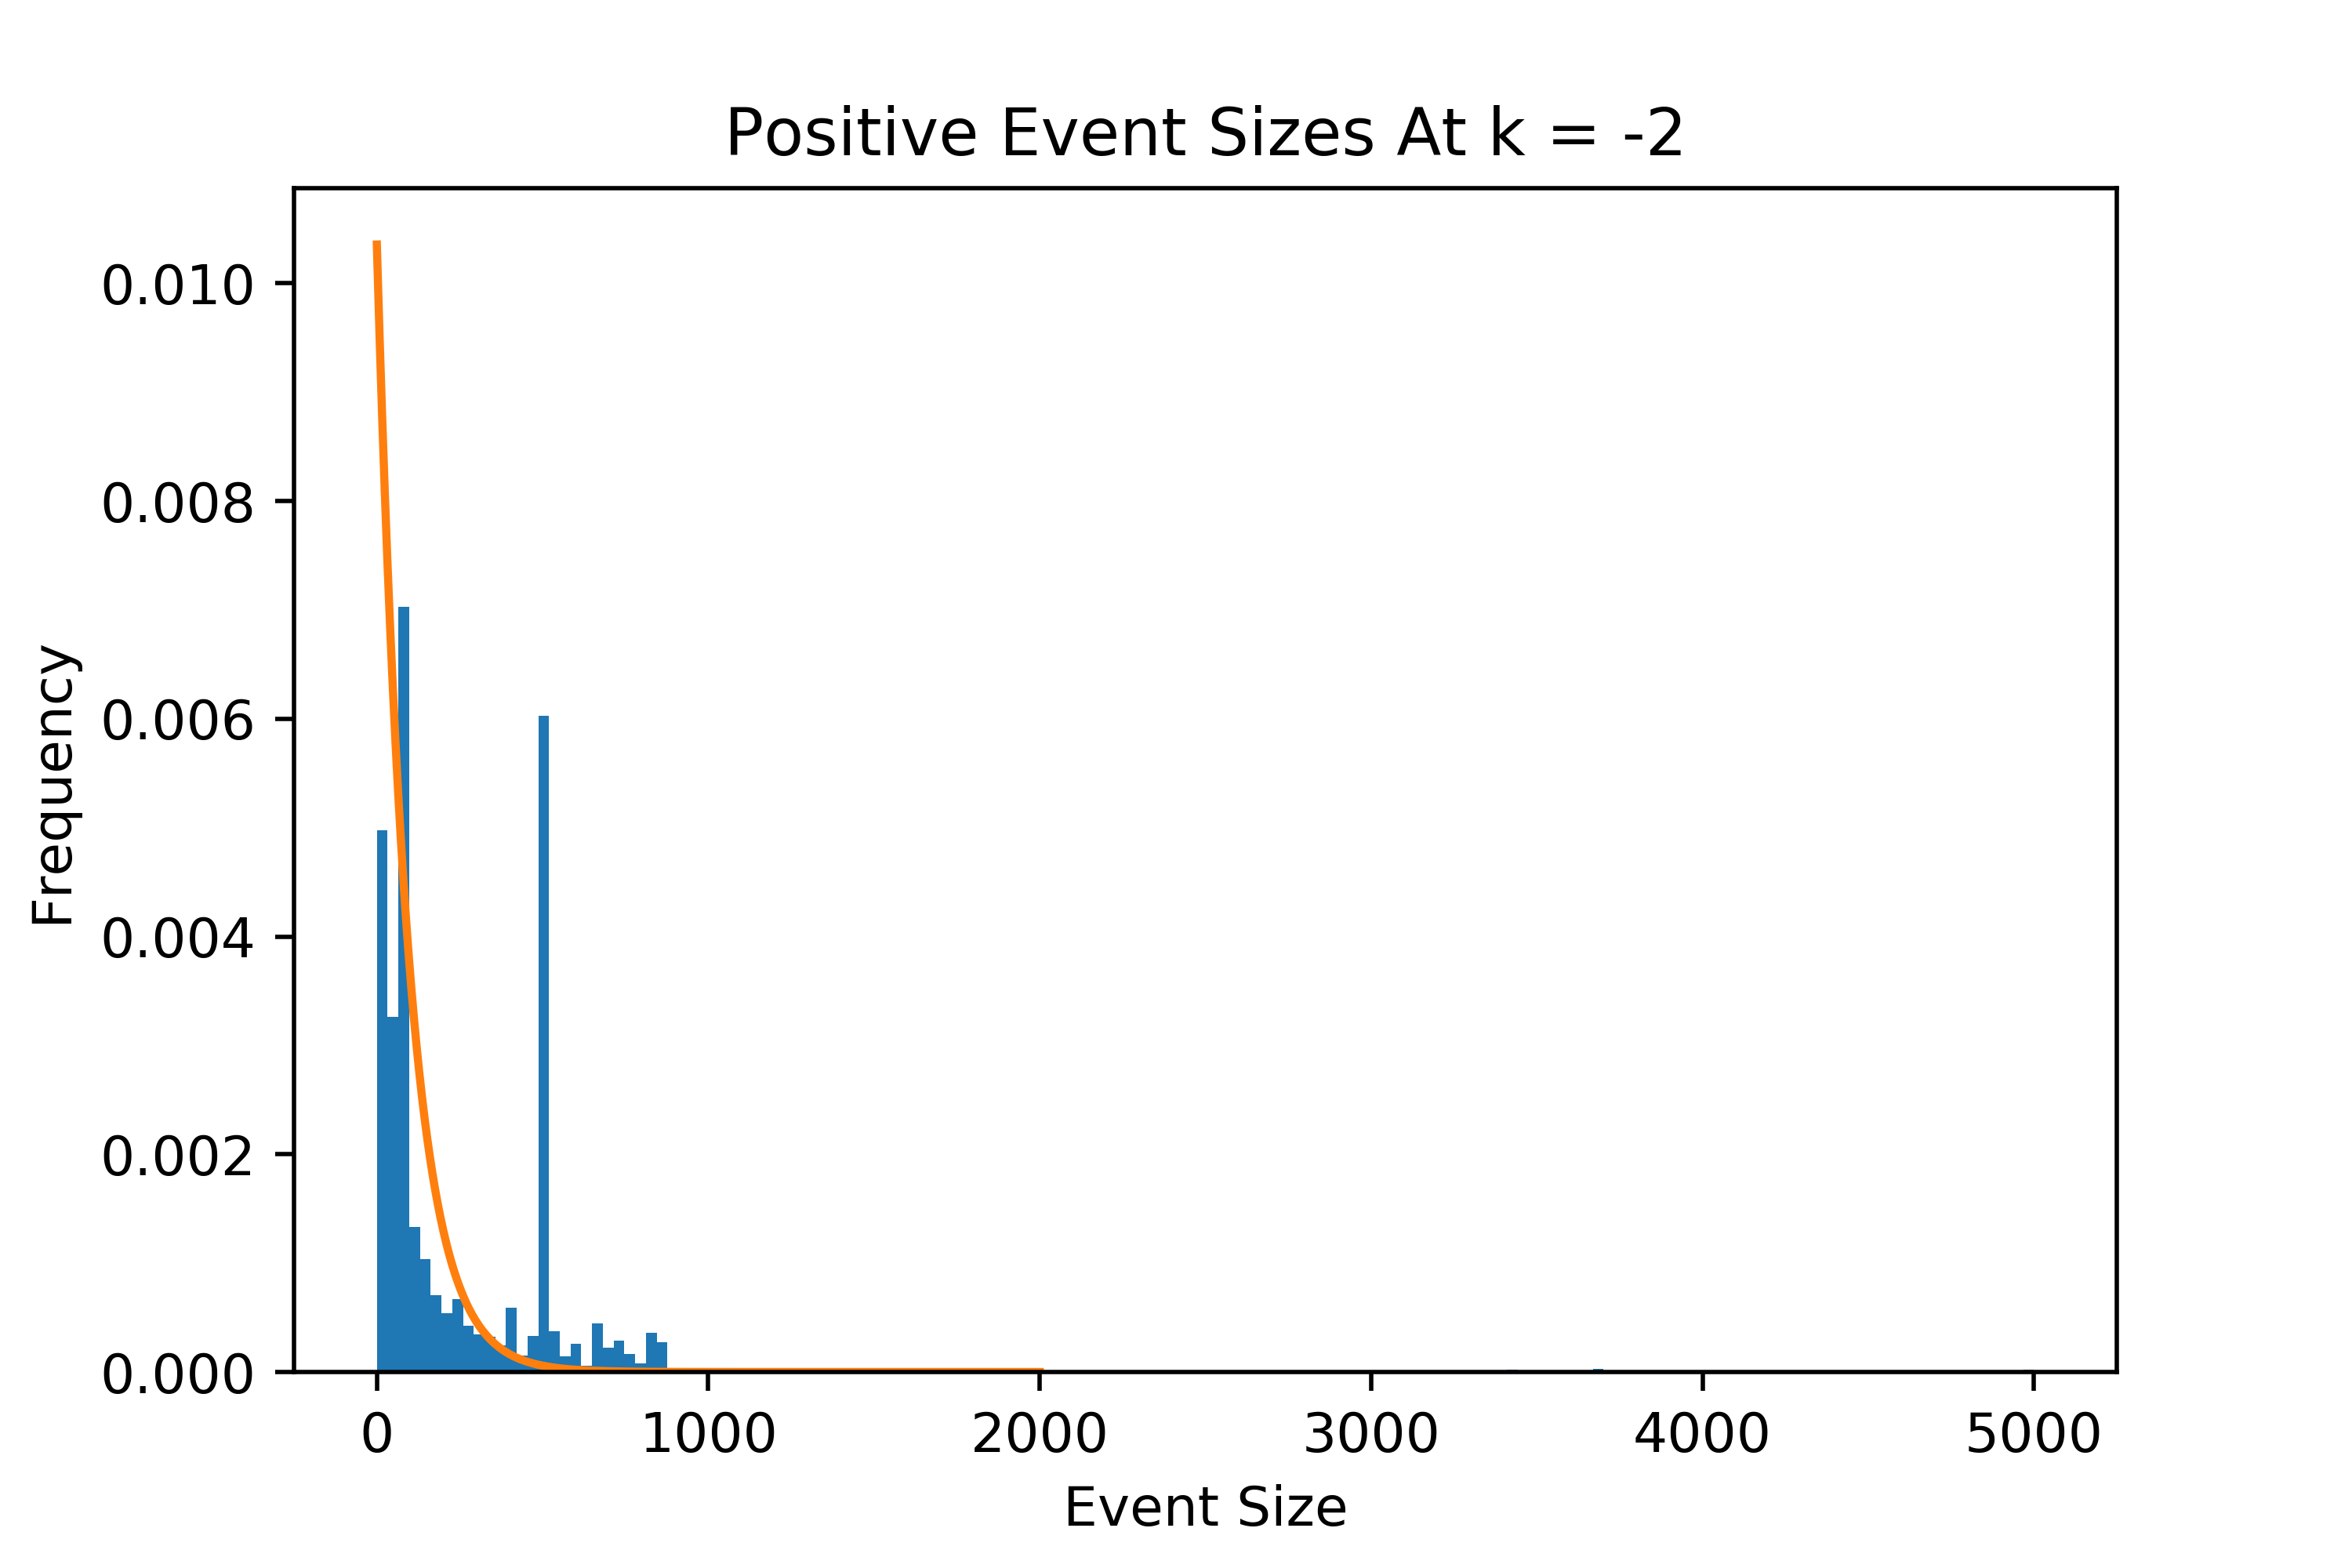
\includegraphics[width=60mm]{Figures/pos_-2.png}}
{}
&
\subf{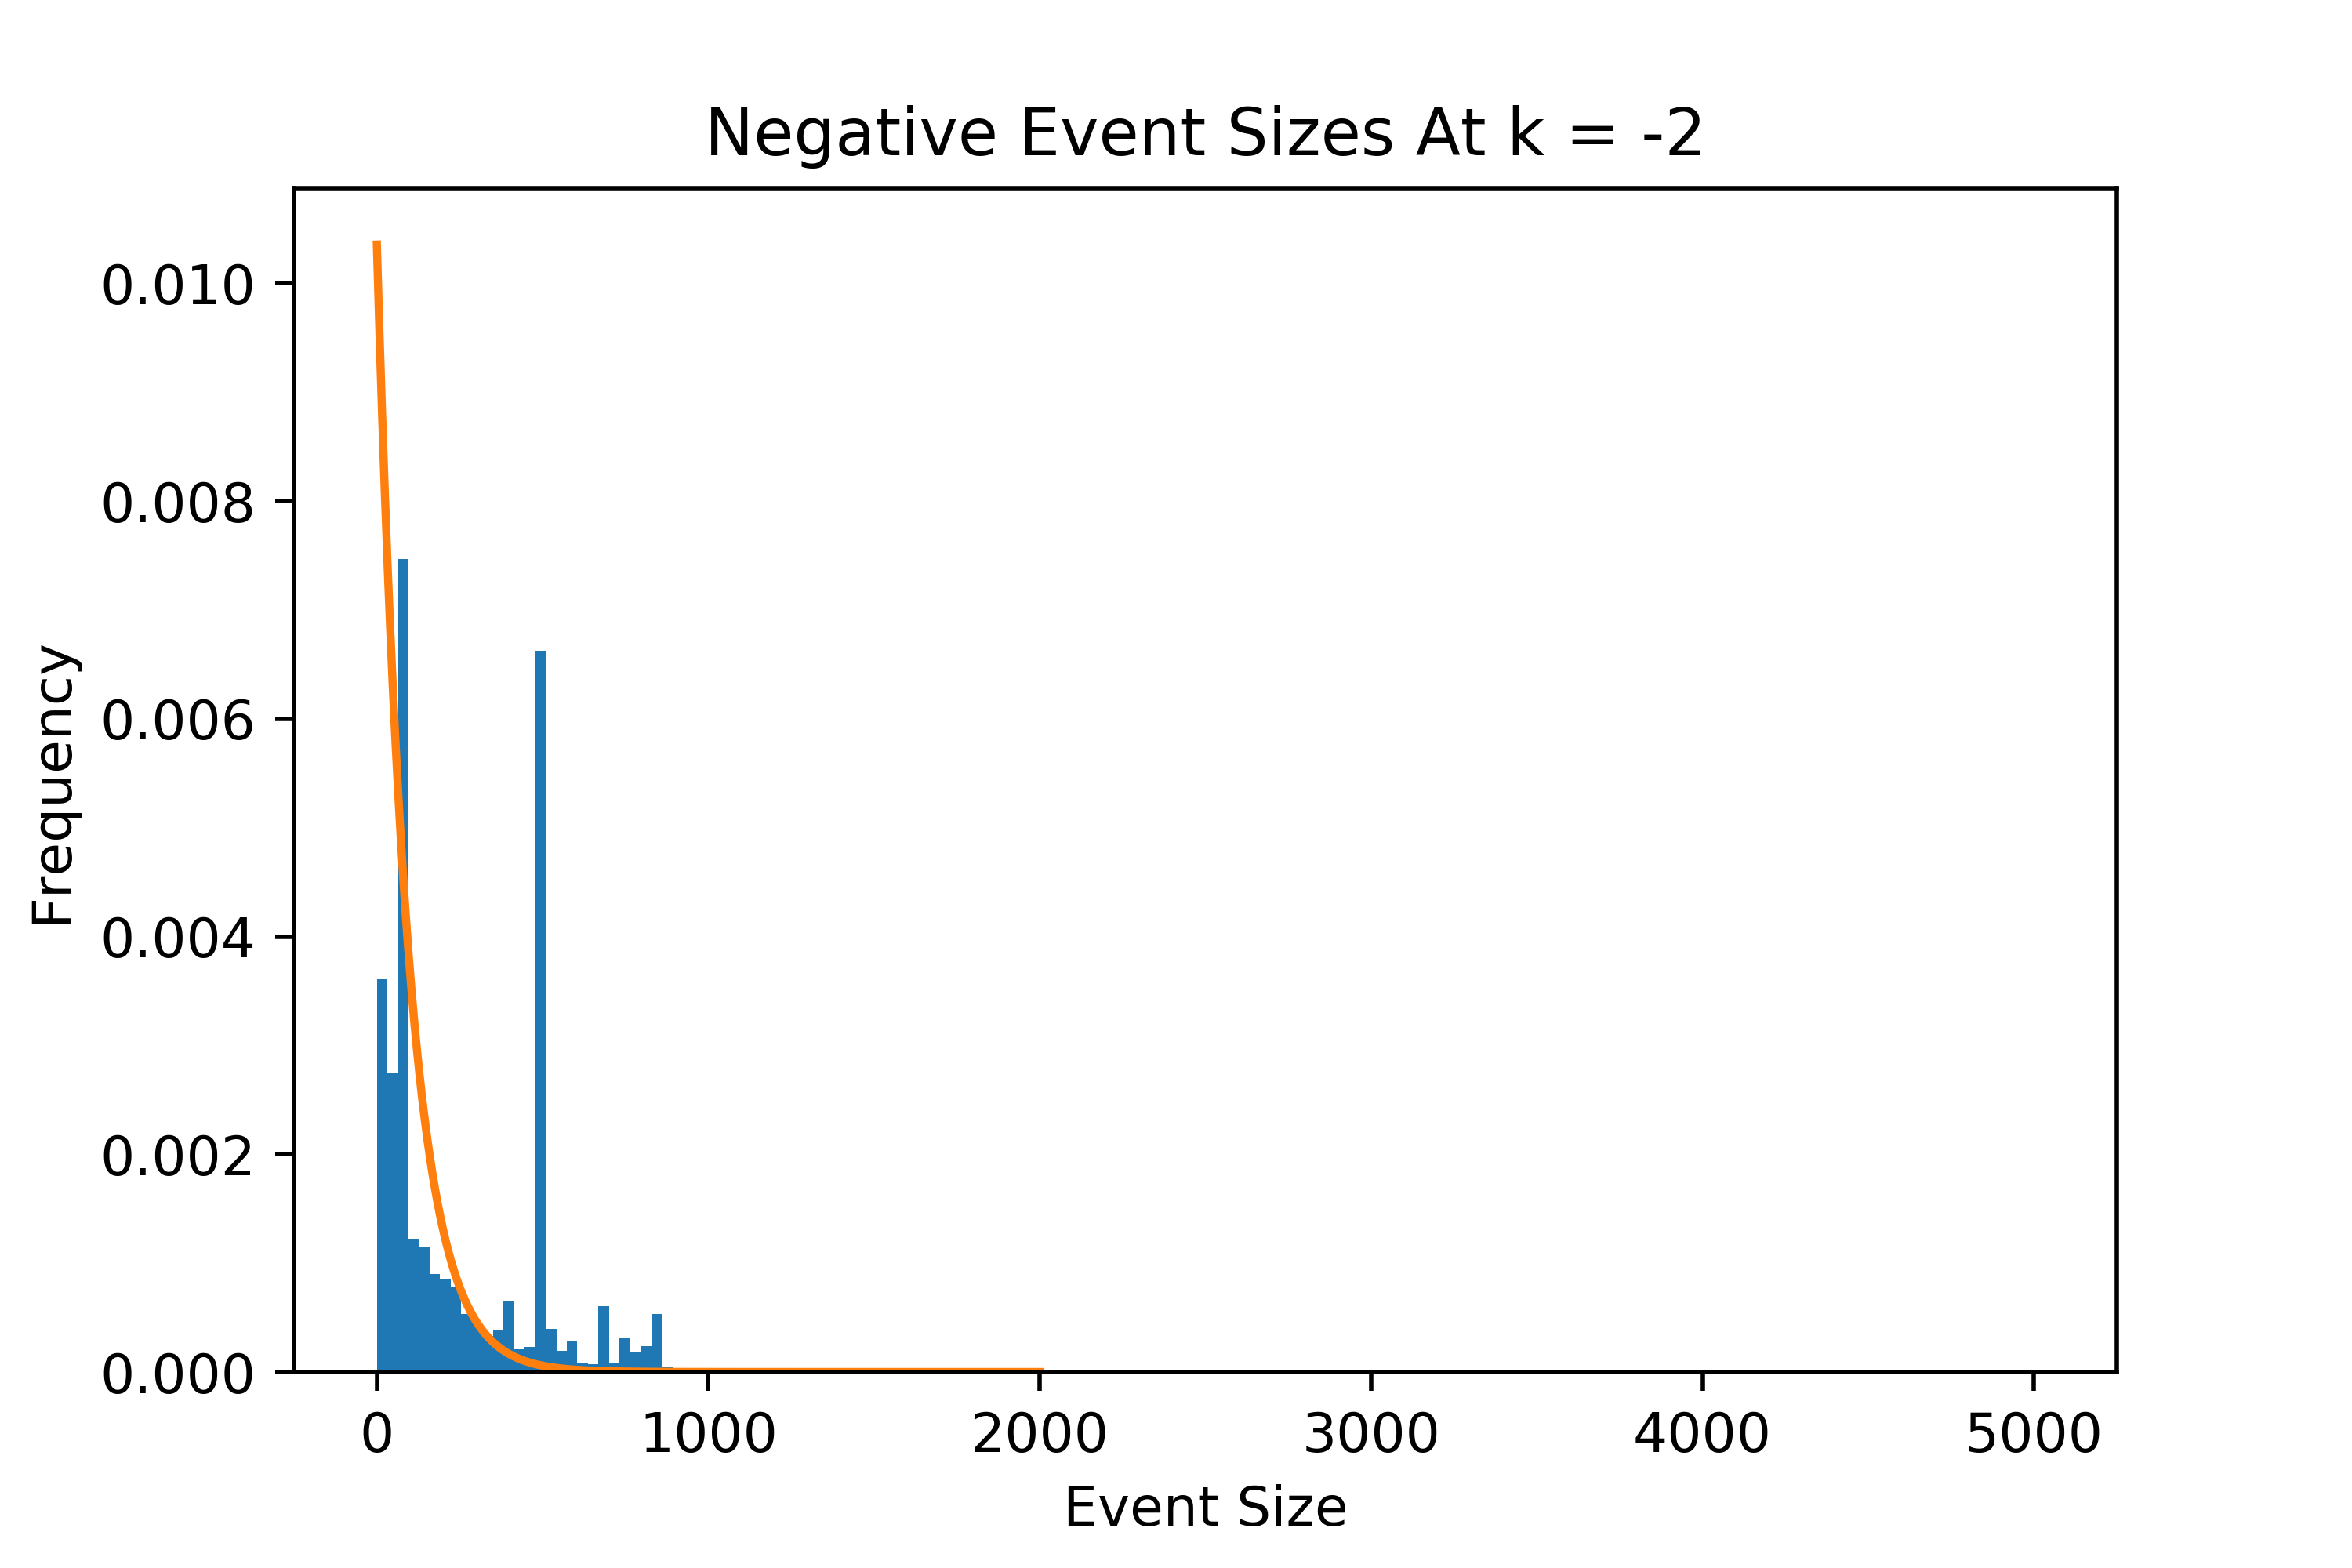
\includegraphics[width=60mm]{Figures/neg_-2.png}}
{}
\\
% \subf{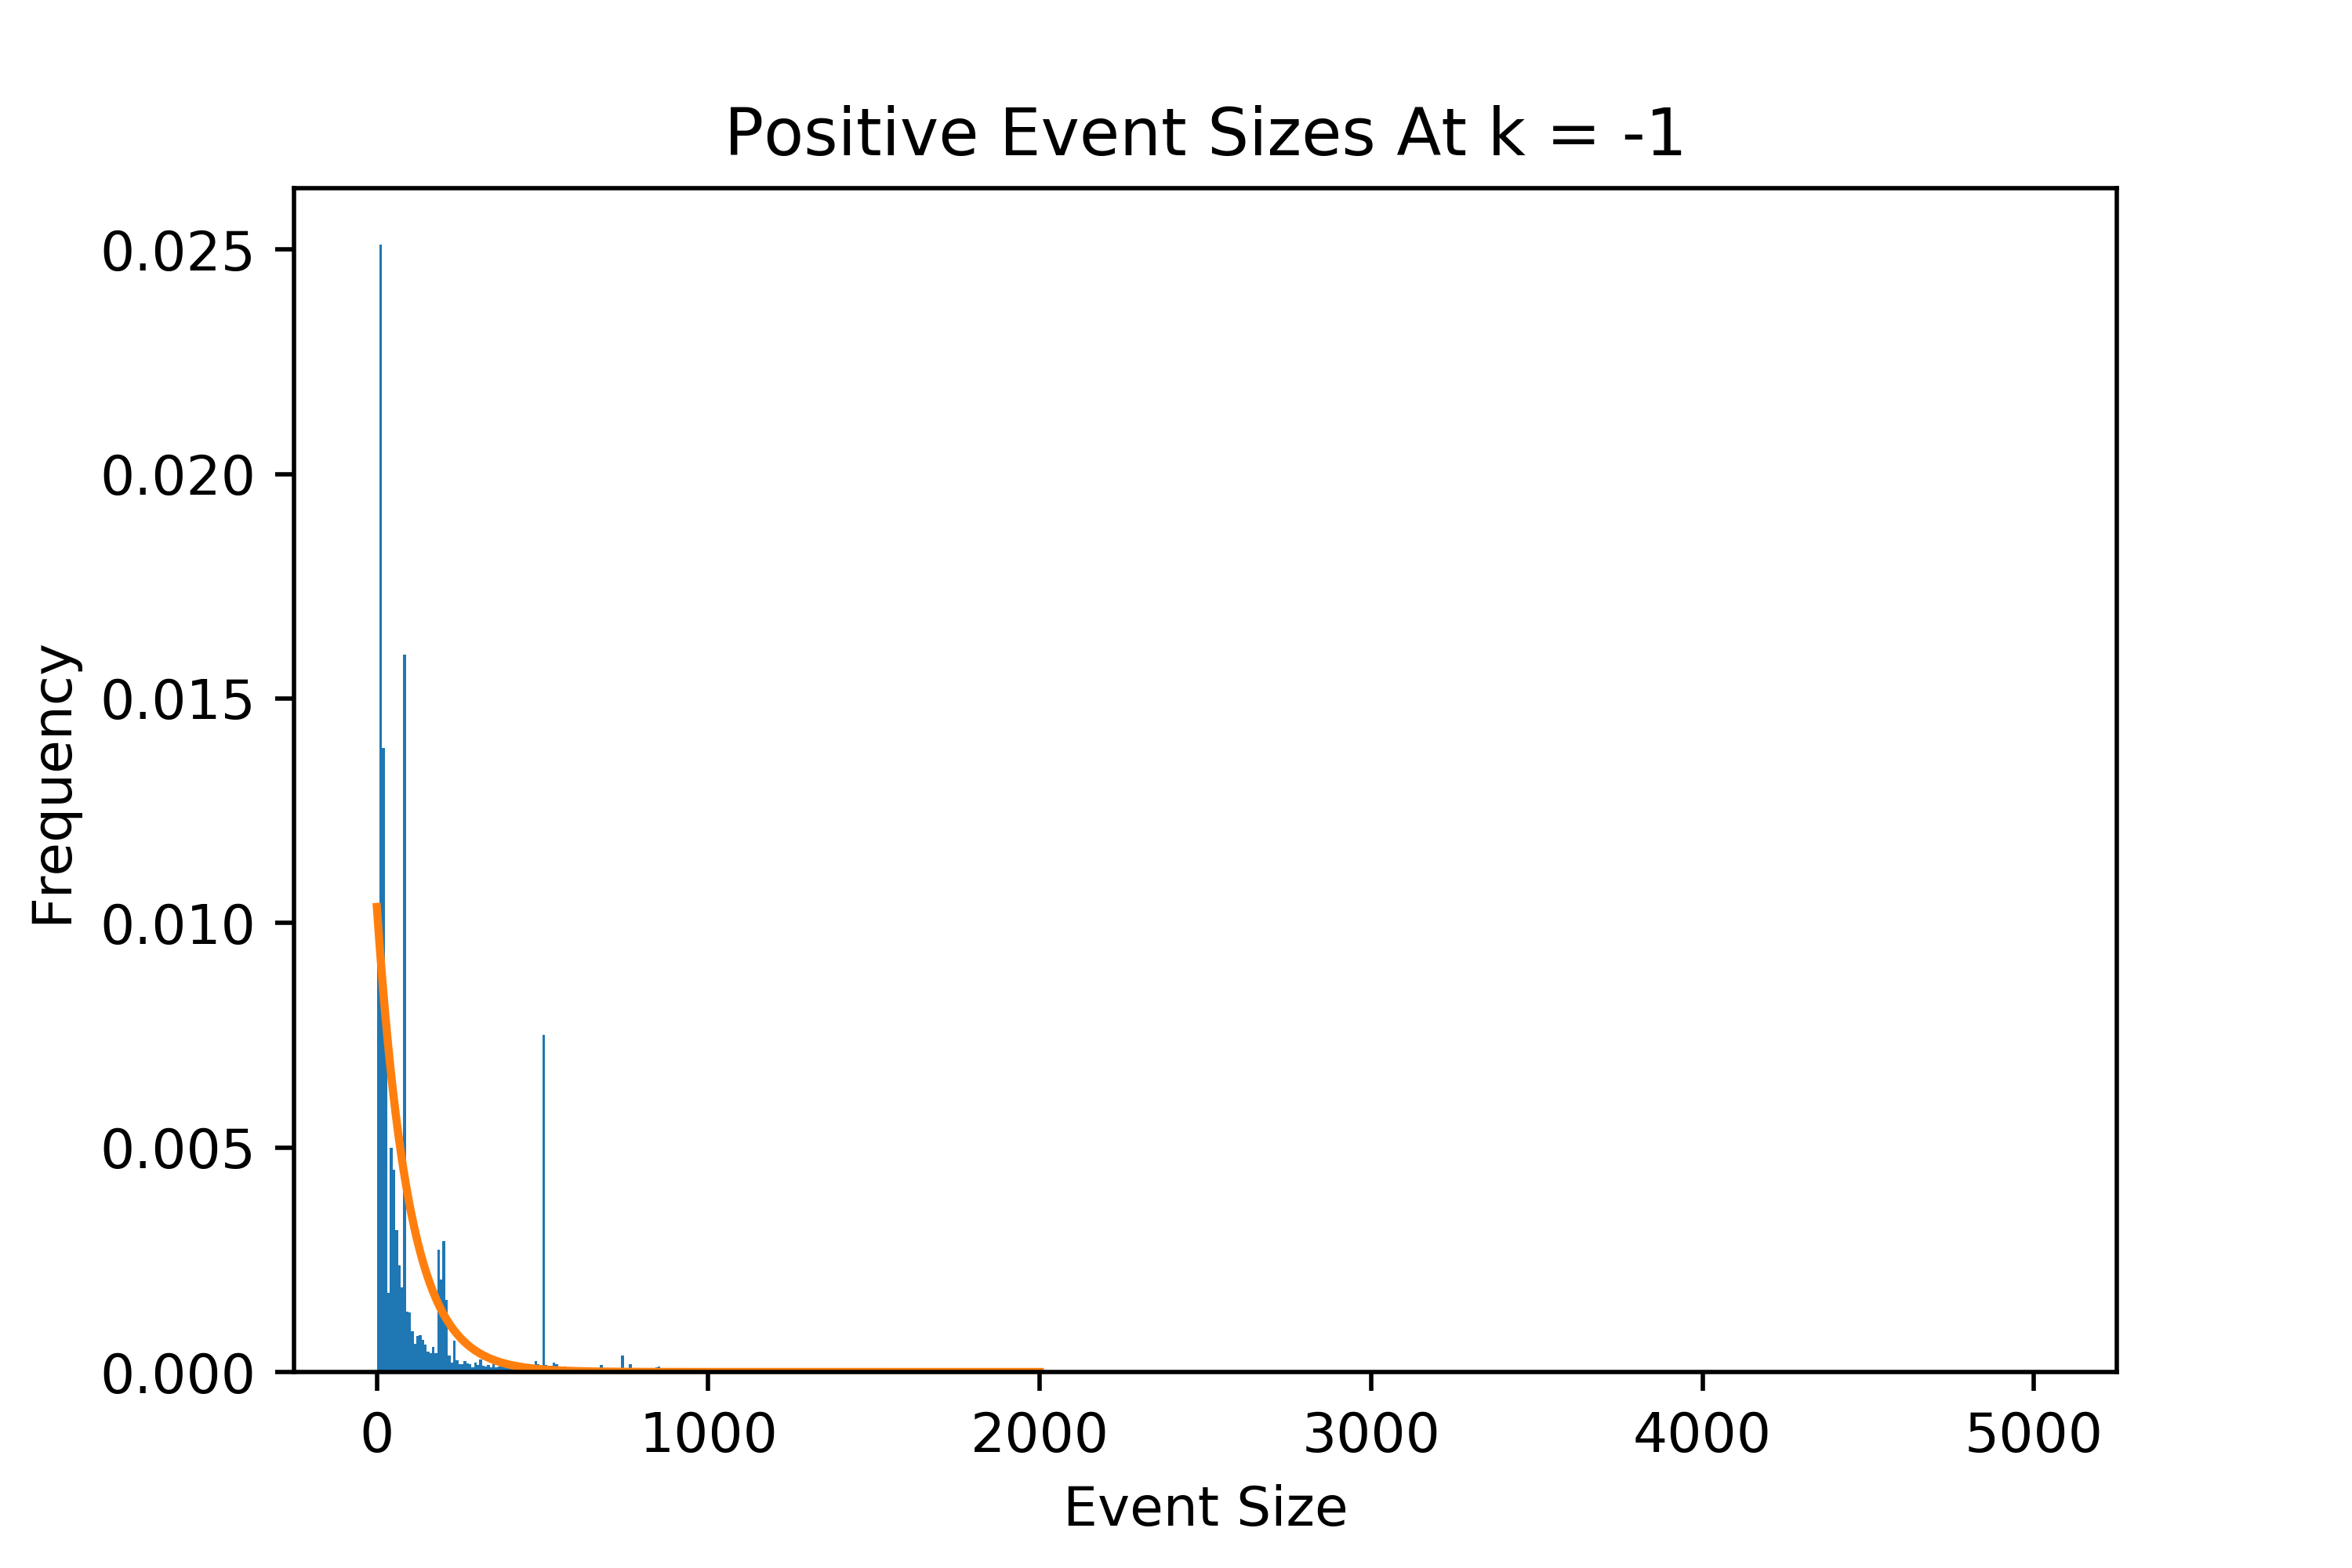
\includegraphics[width=60mm]{Figures/pos_-1.png}}
% {}
% &
% \subf{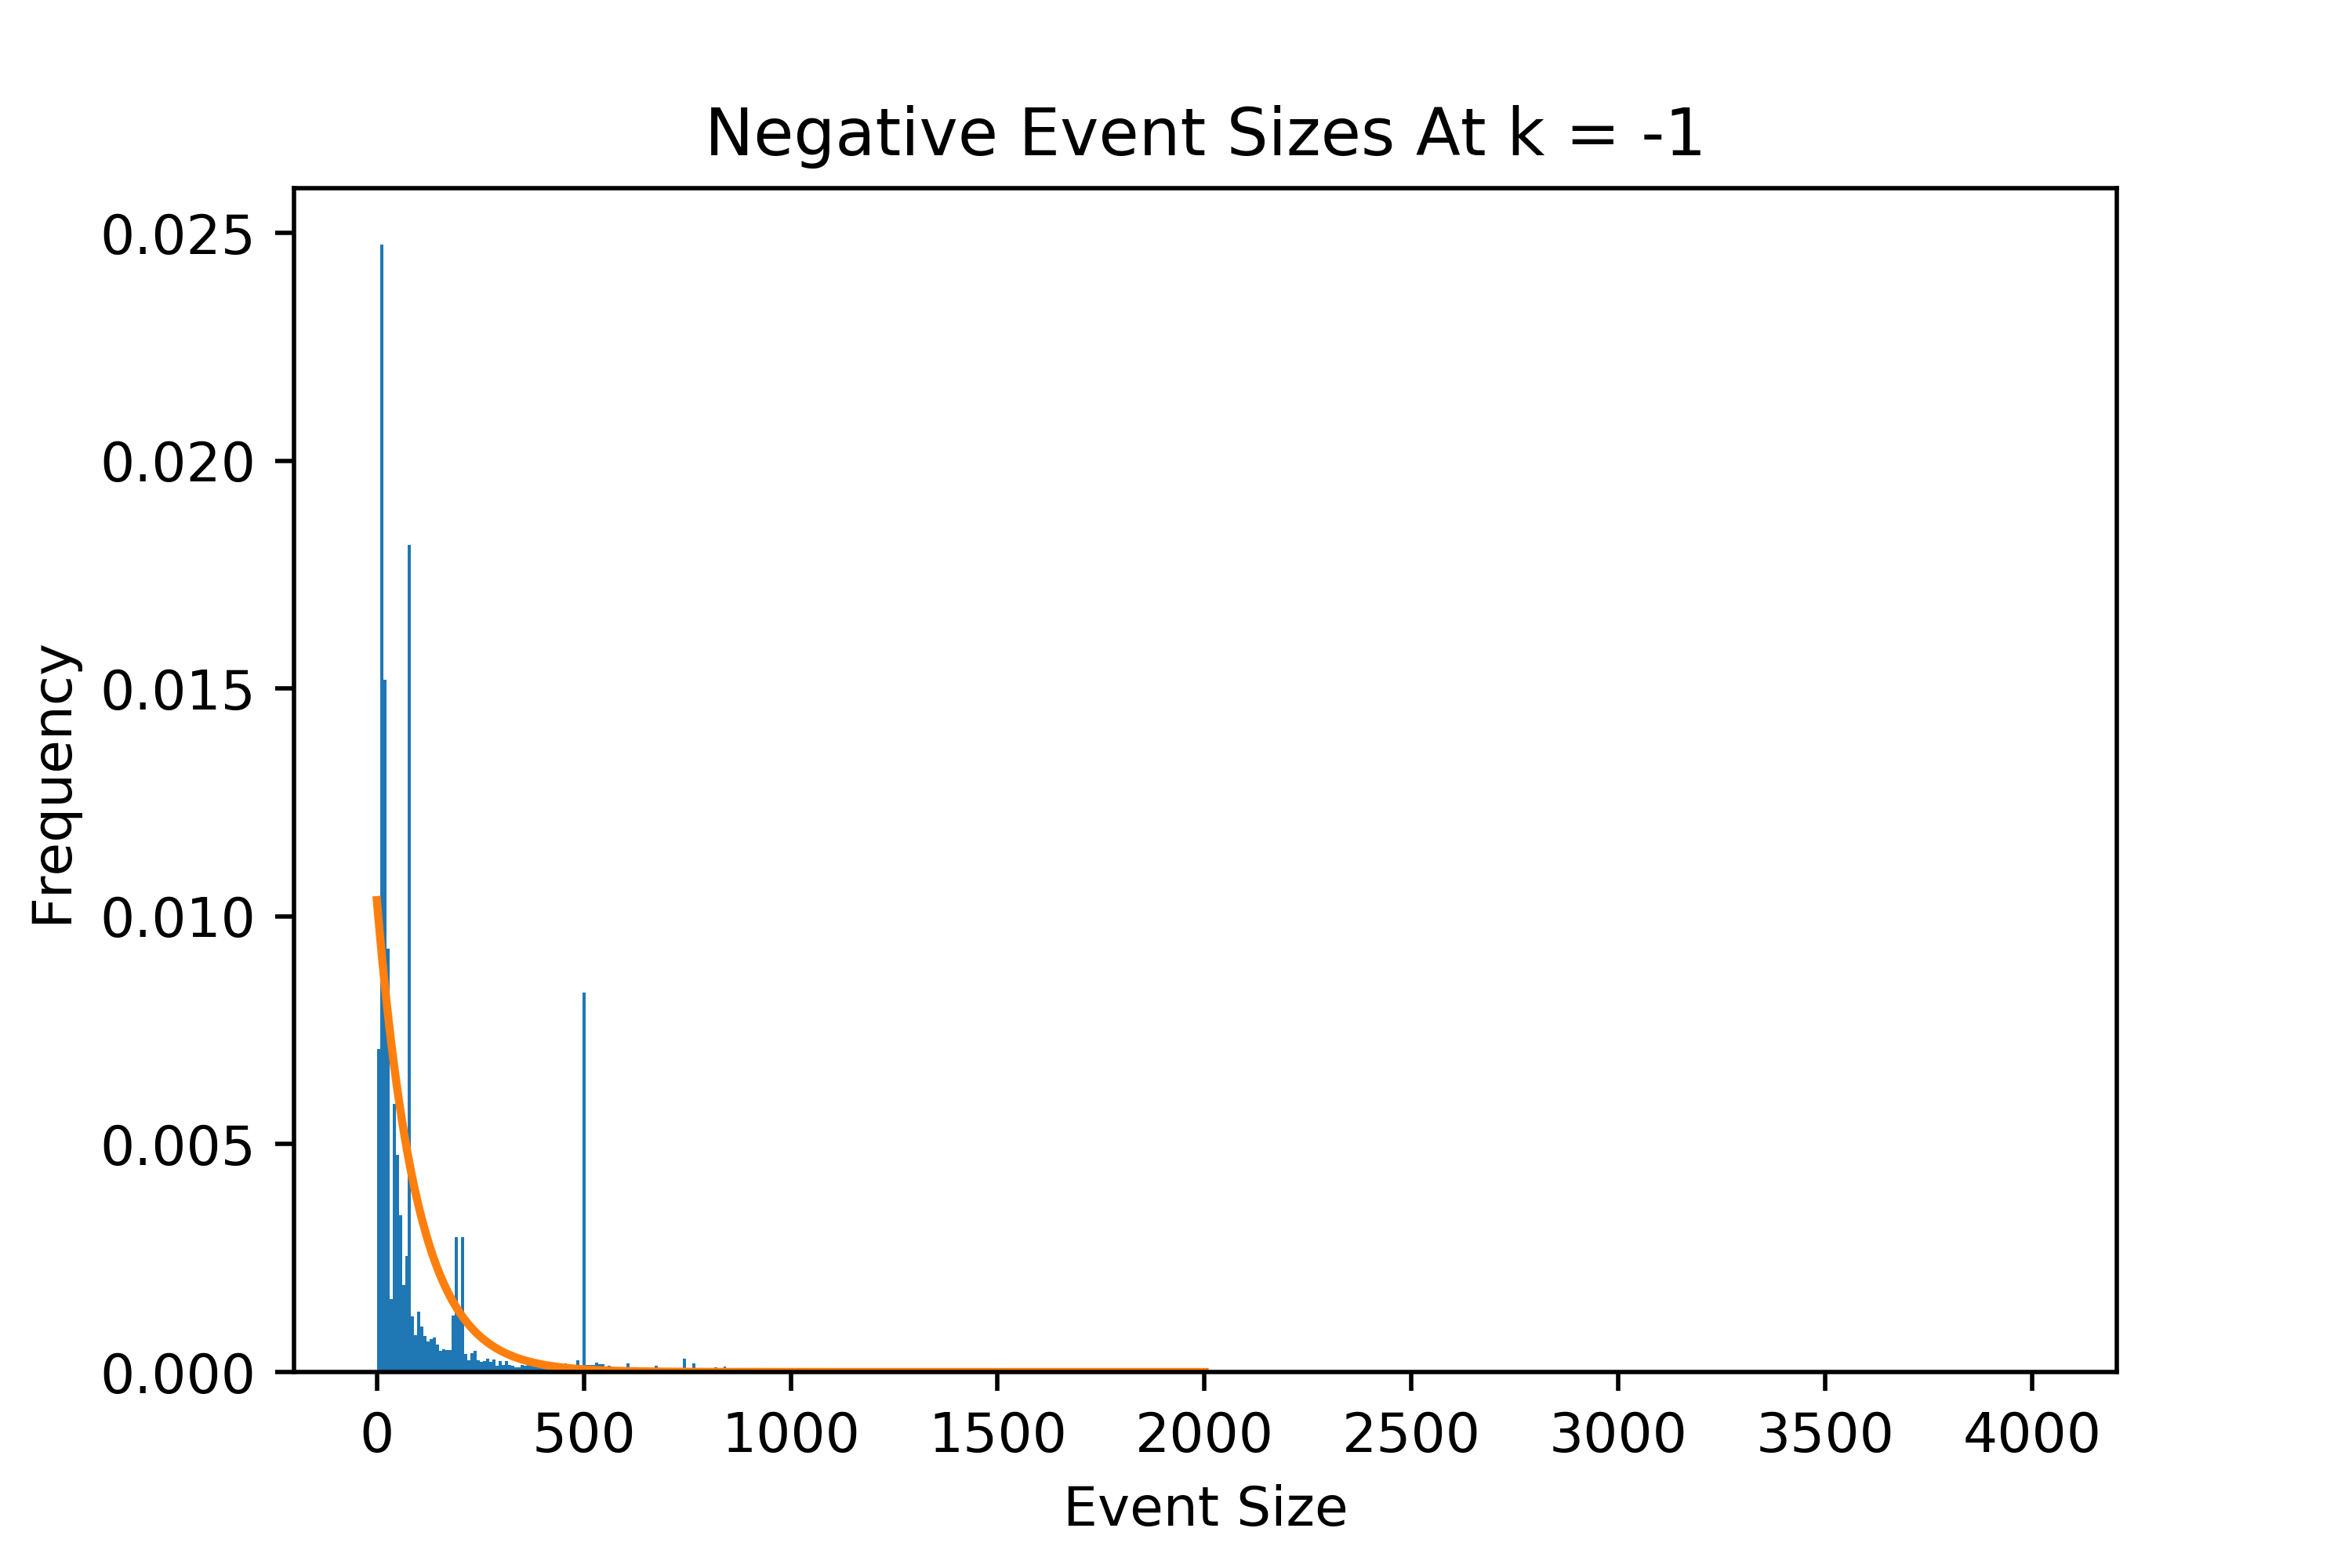
\includegraphics[width=60mm]{Figures/neg_-1.png}}
% {}
% \\
% \subf{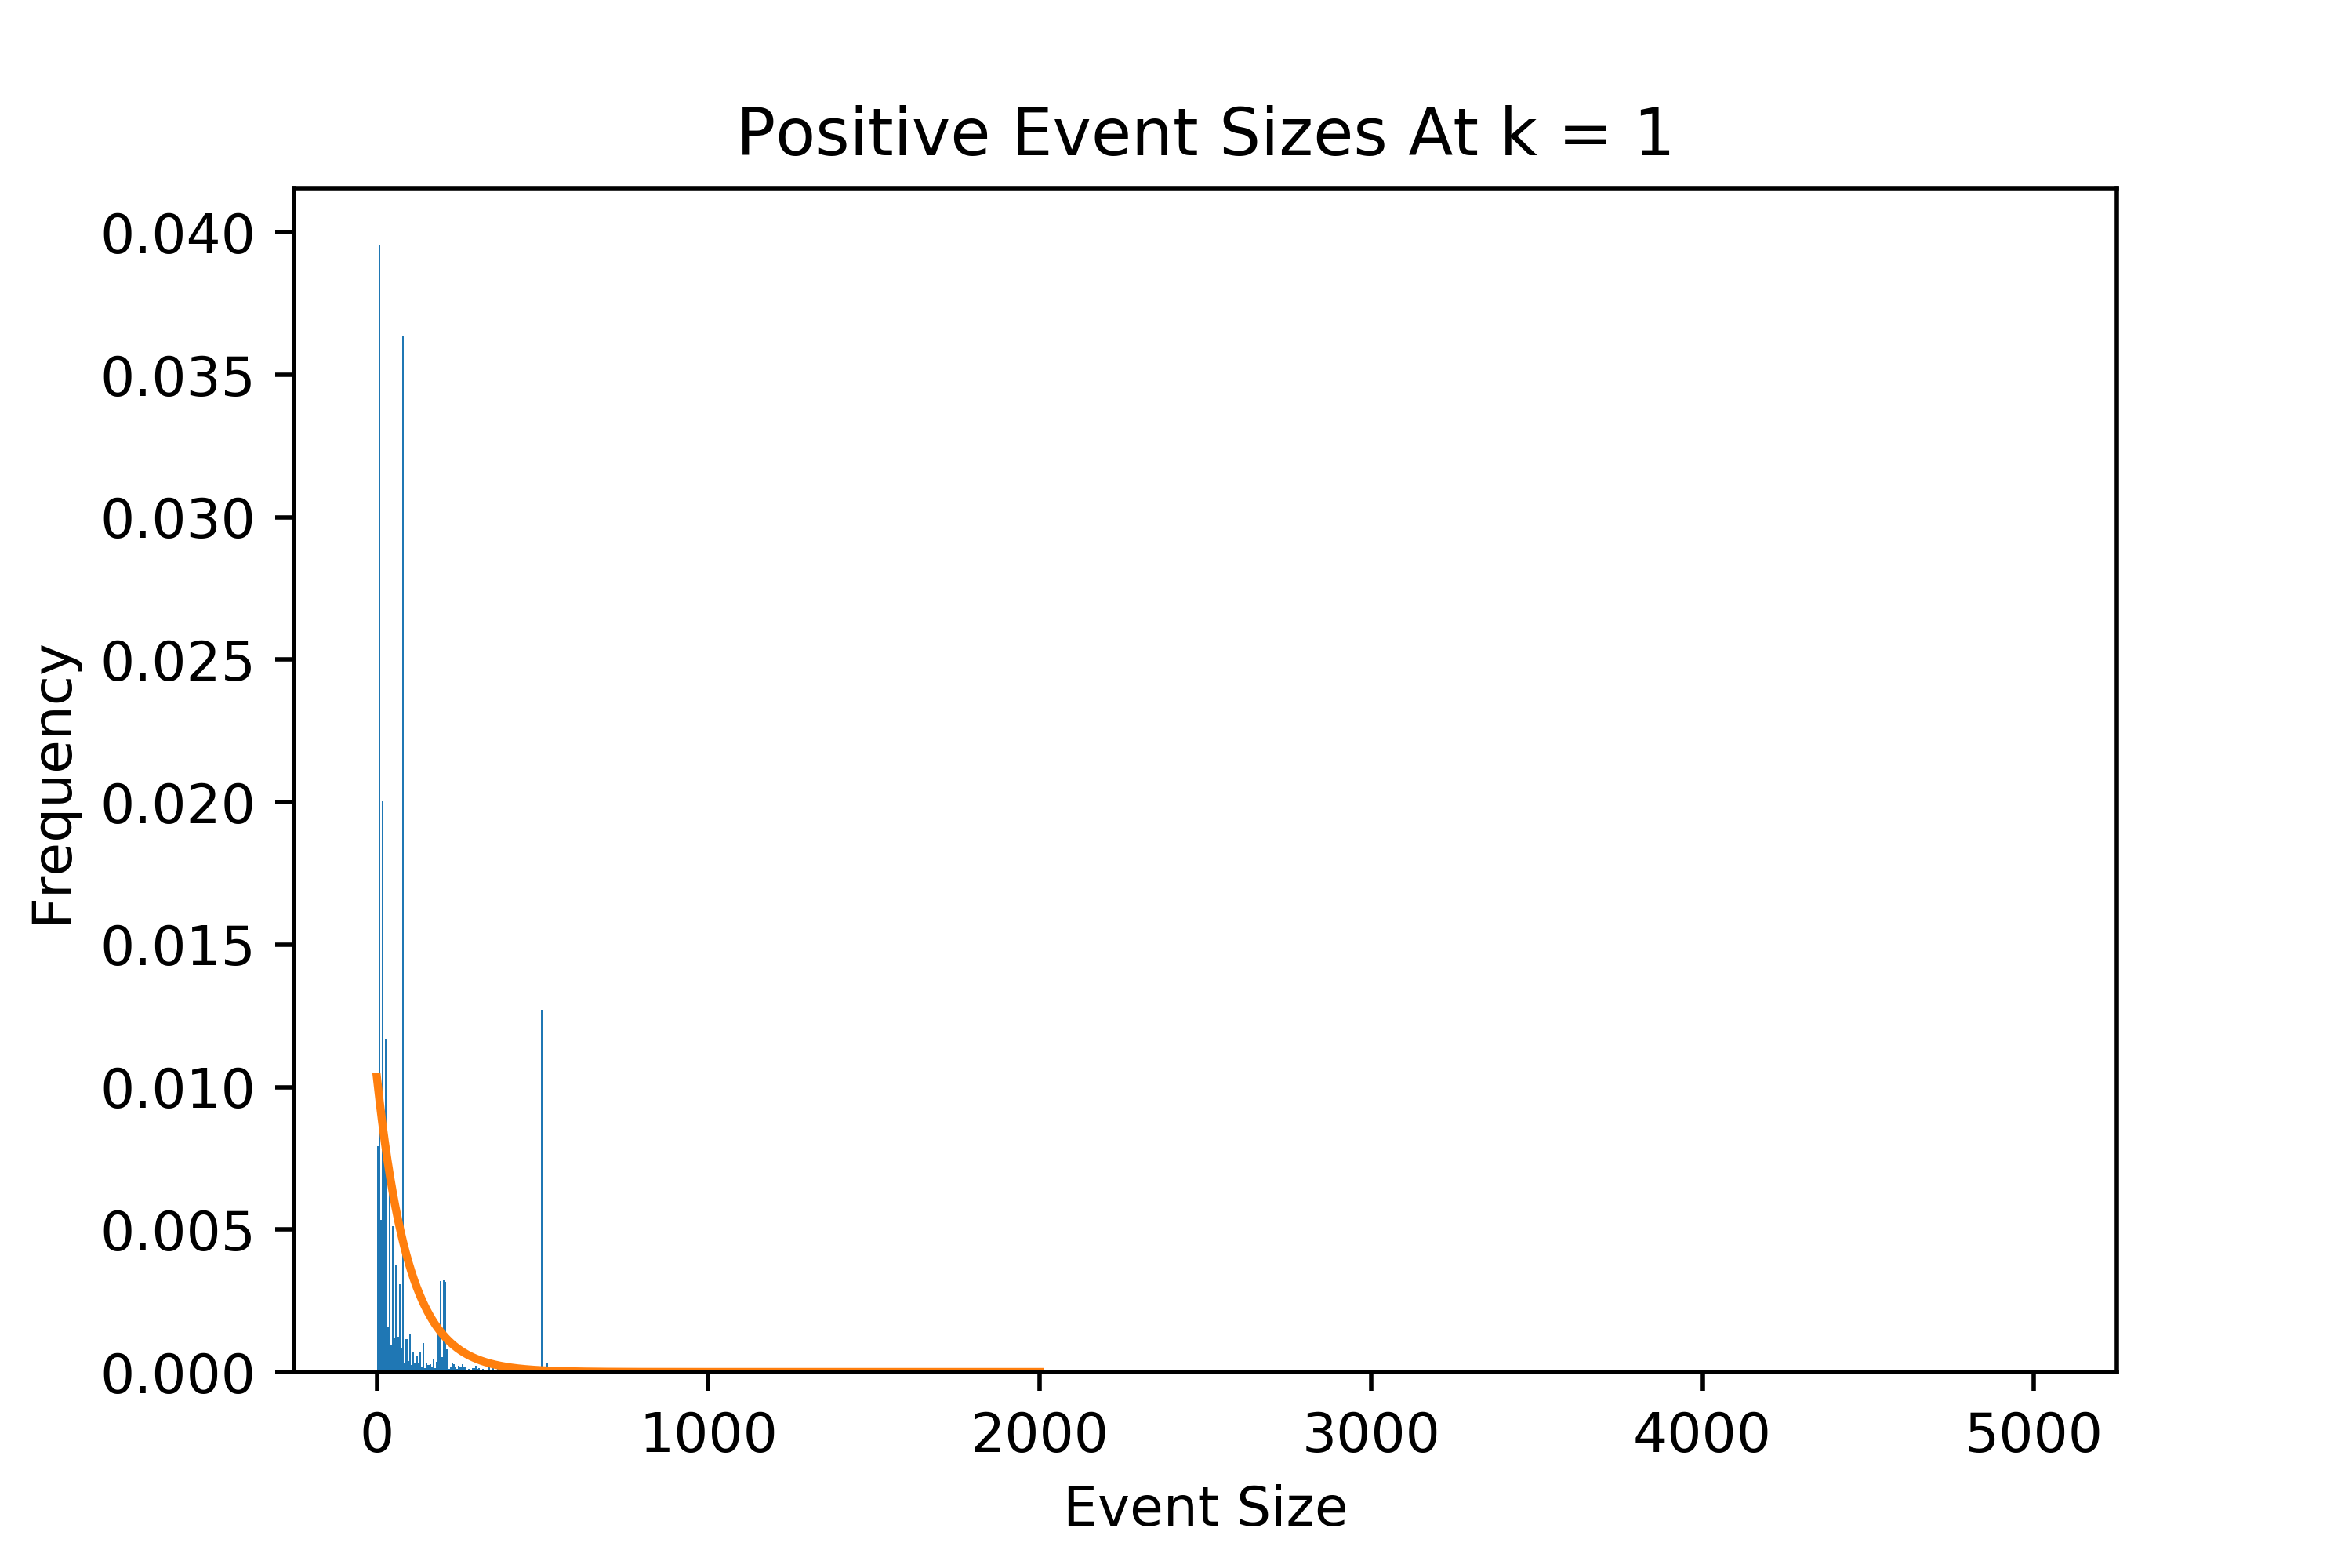
\includegraphics[width=60mm]{Figures/pos_1.png}}
% {}
% &
% \subf{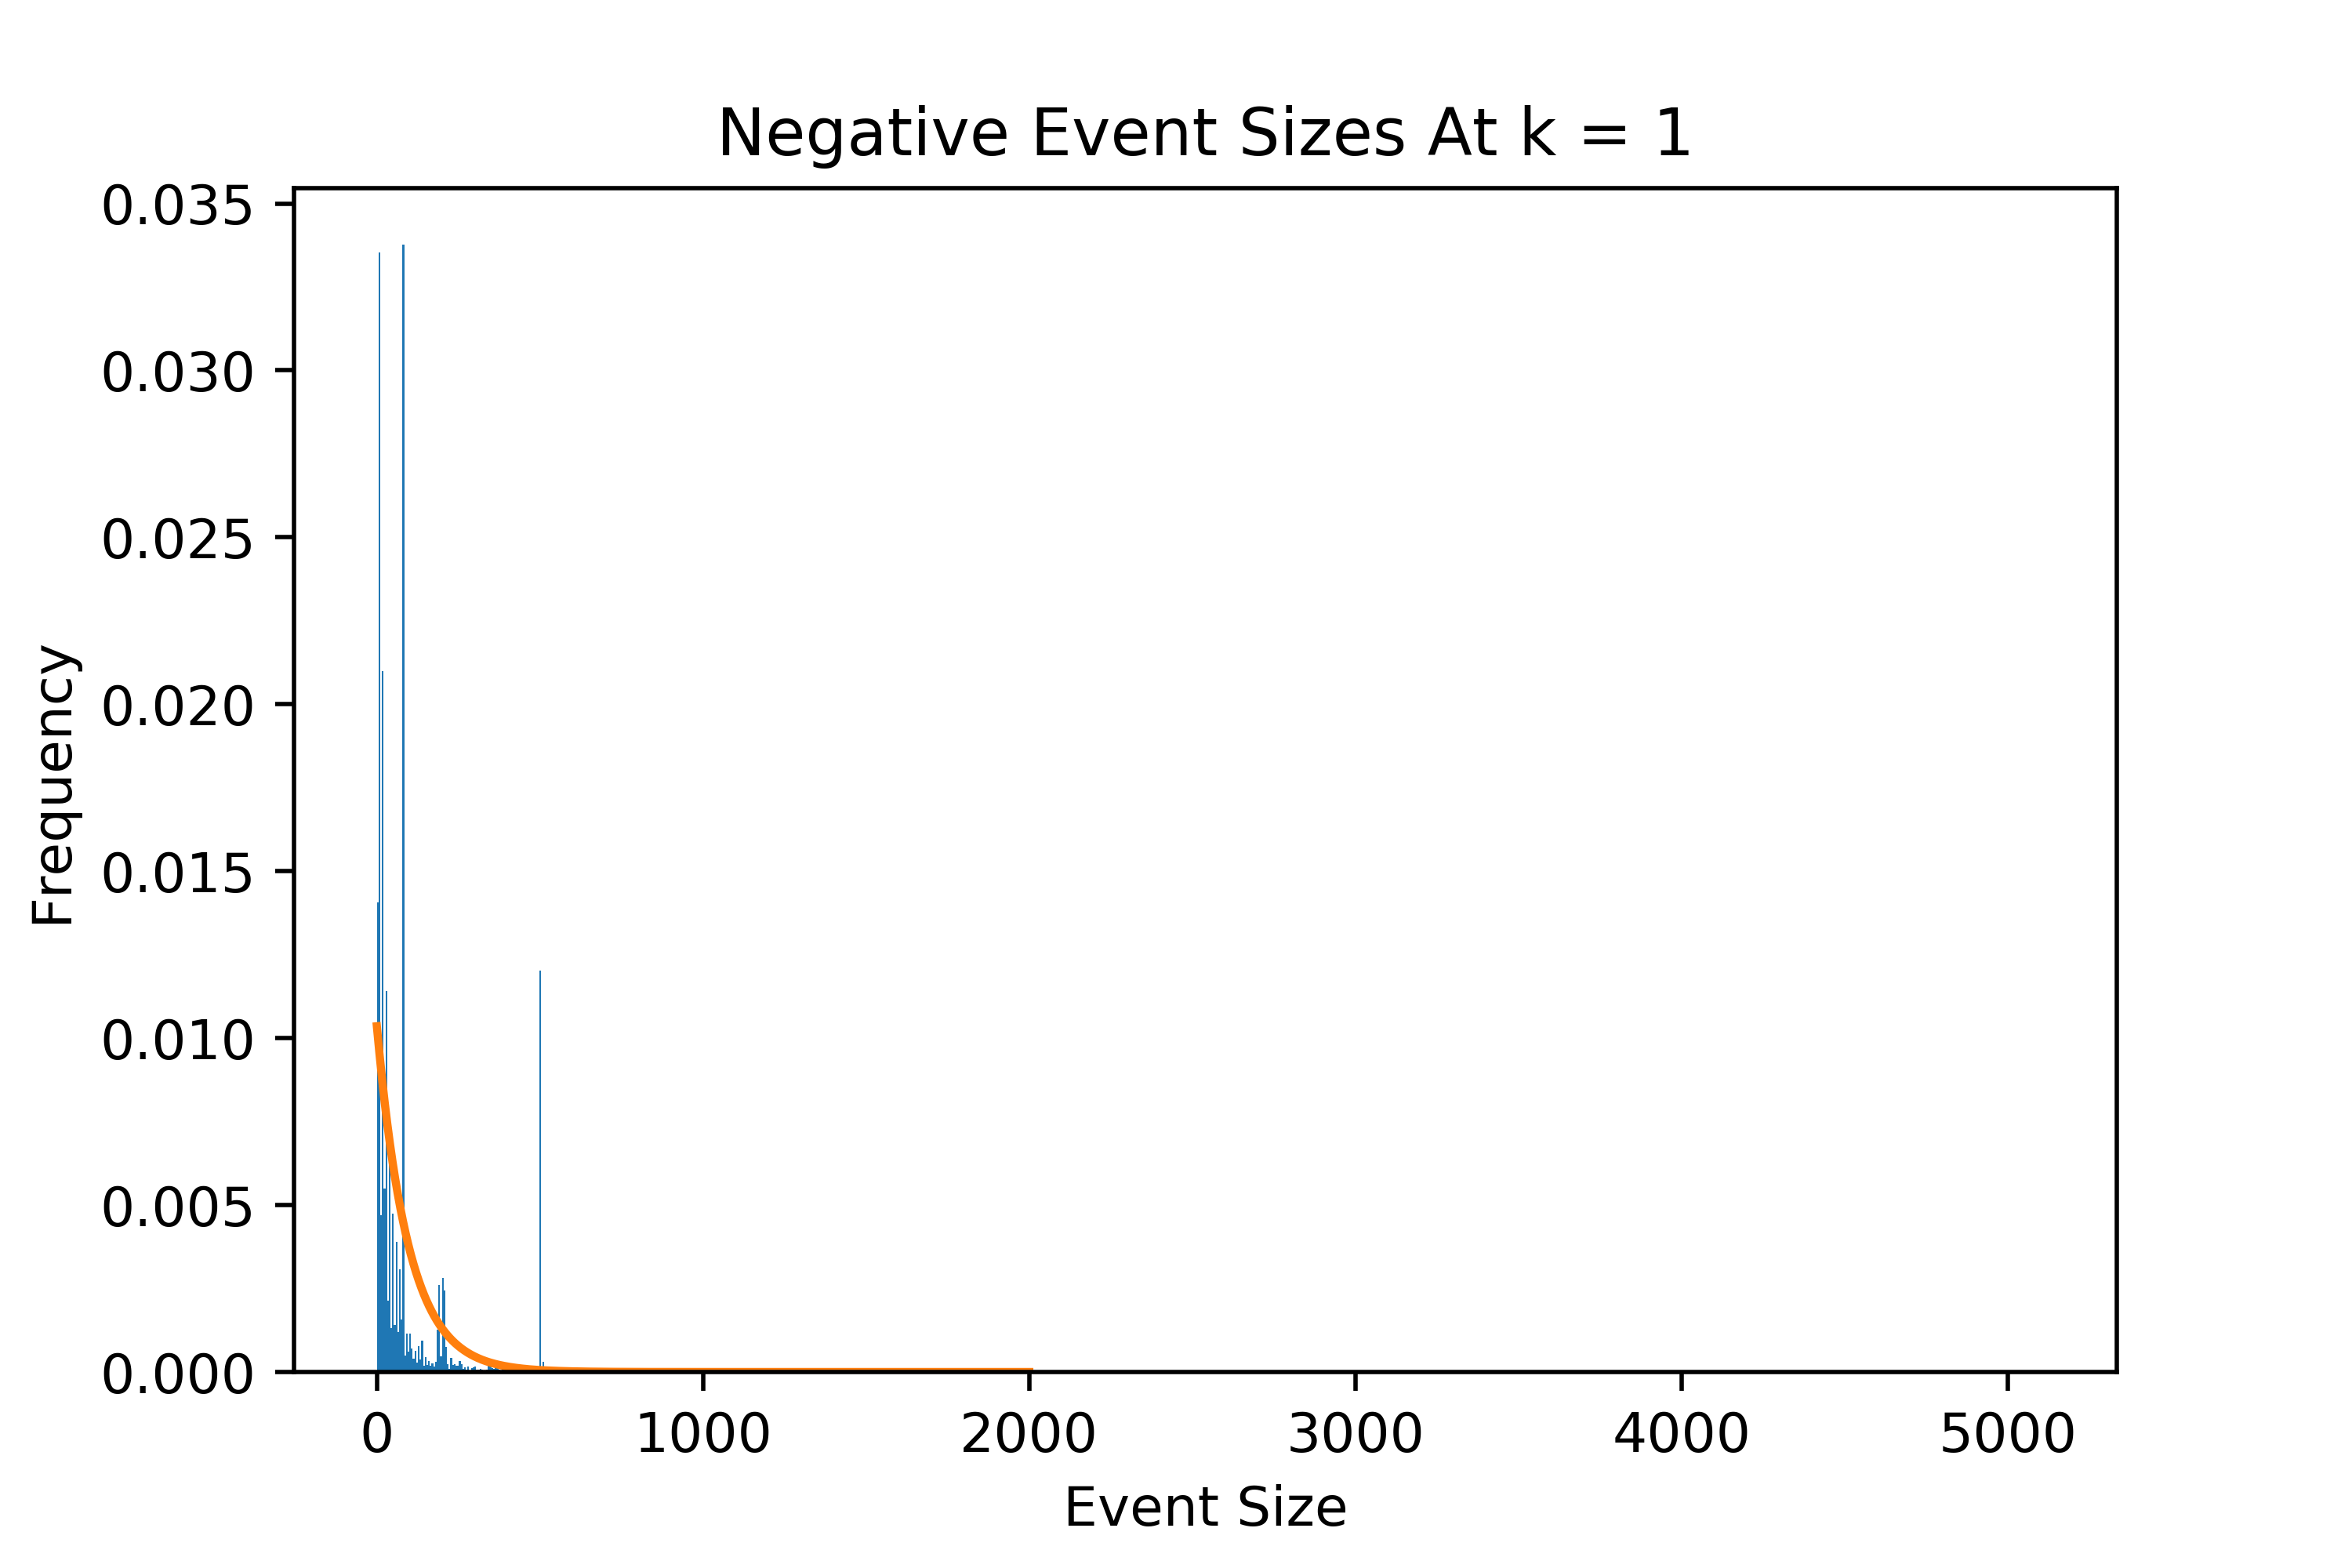
\includegraphics[width=60mm]{Figures/neg_1.png}}
% {}
% \\
% \subf{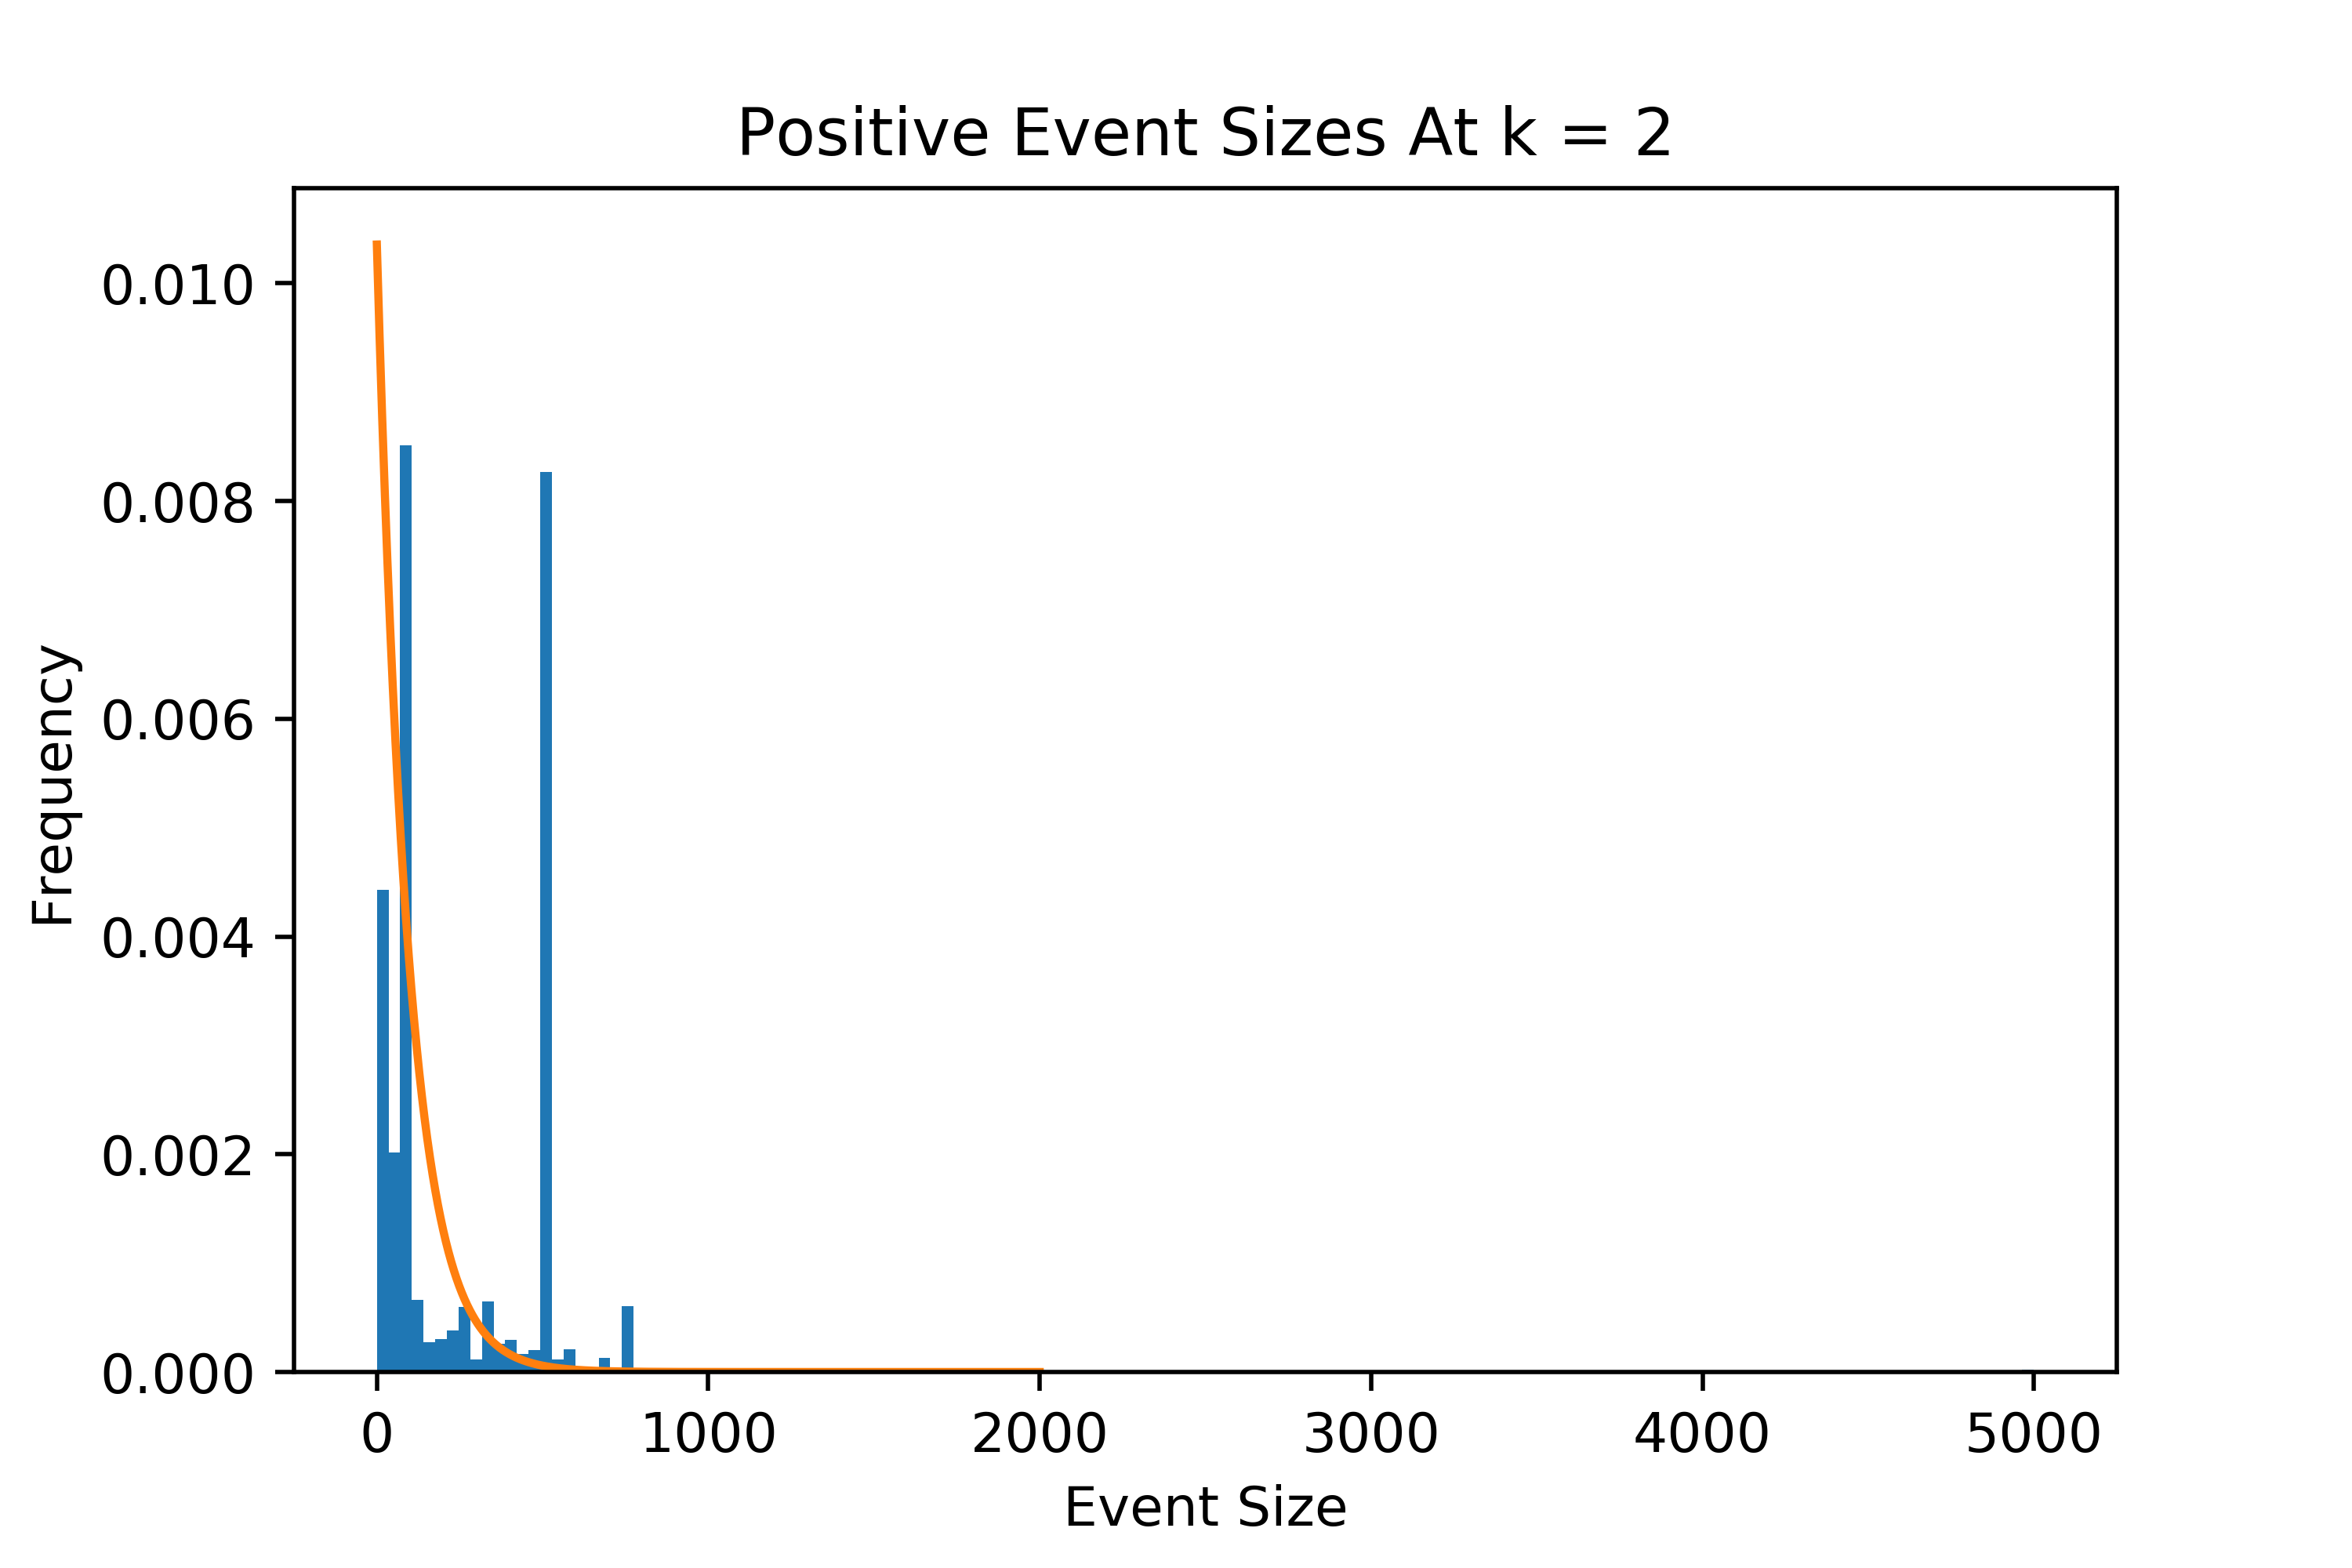
\includegraphics[width=60mm]{Figures/pos_2.png}}
% {}
% &
% \subf{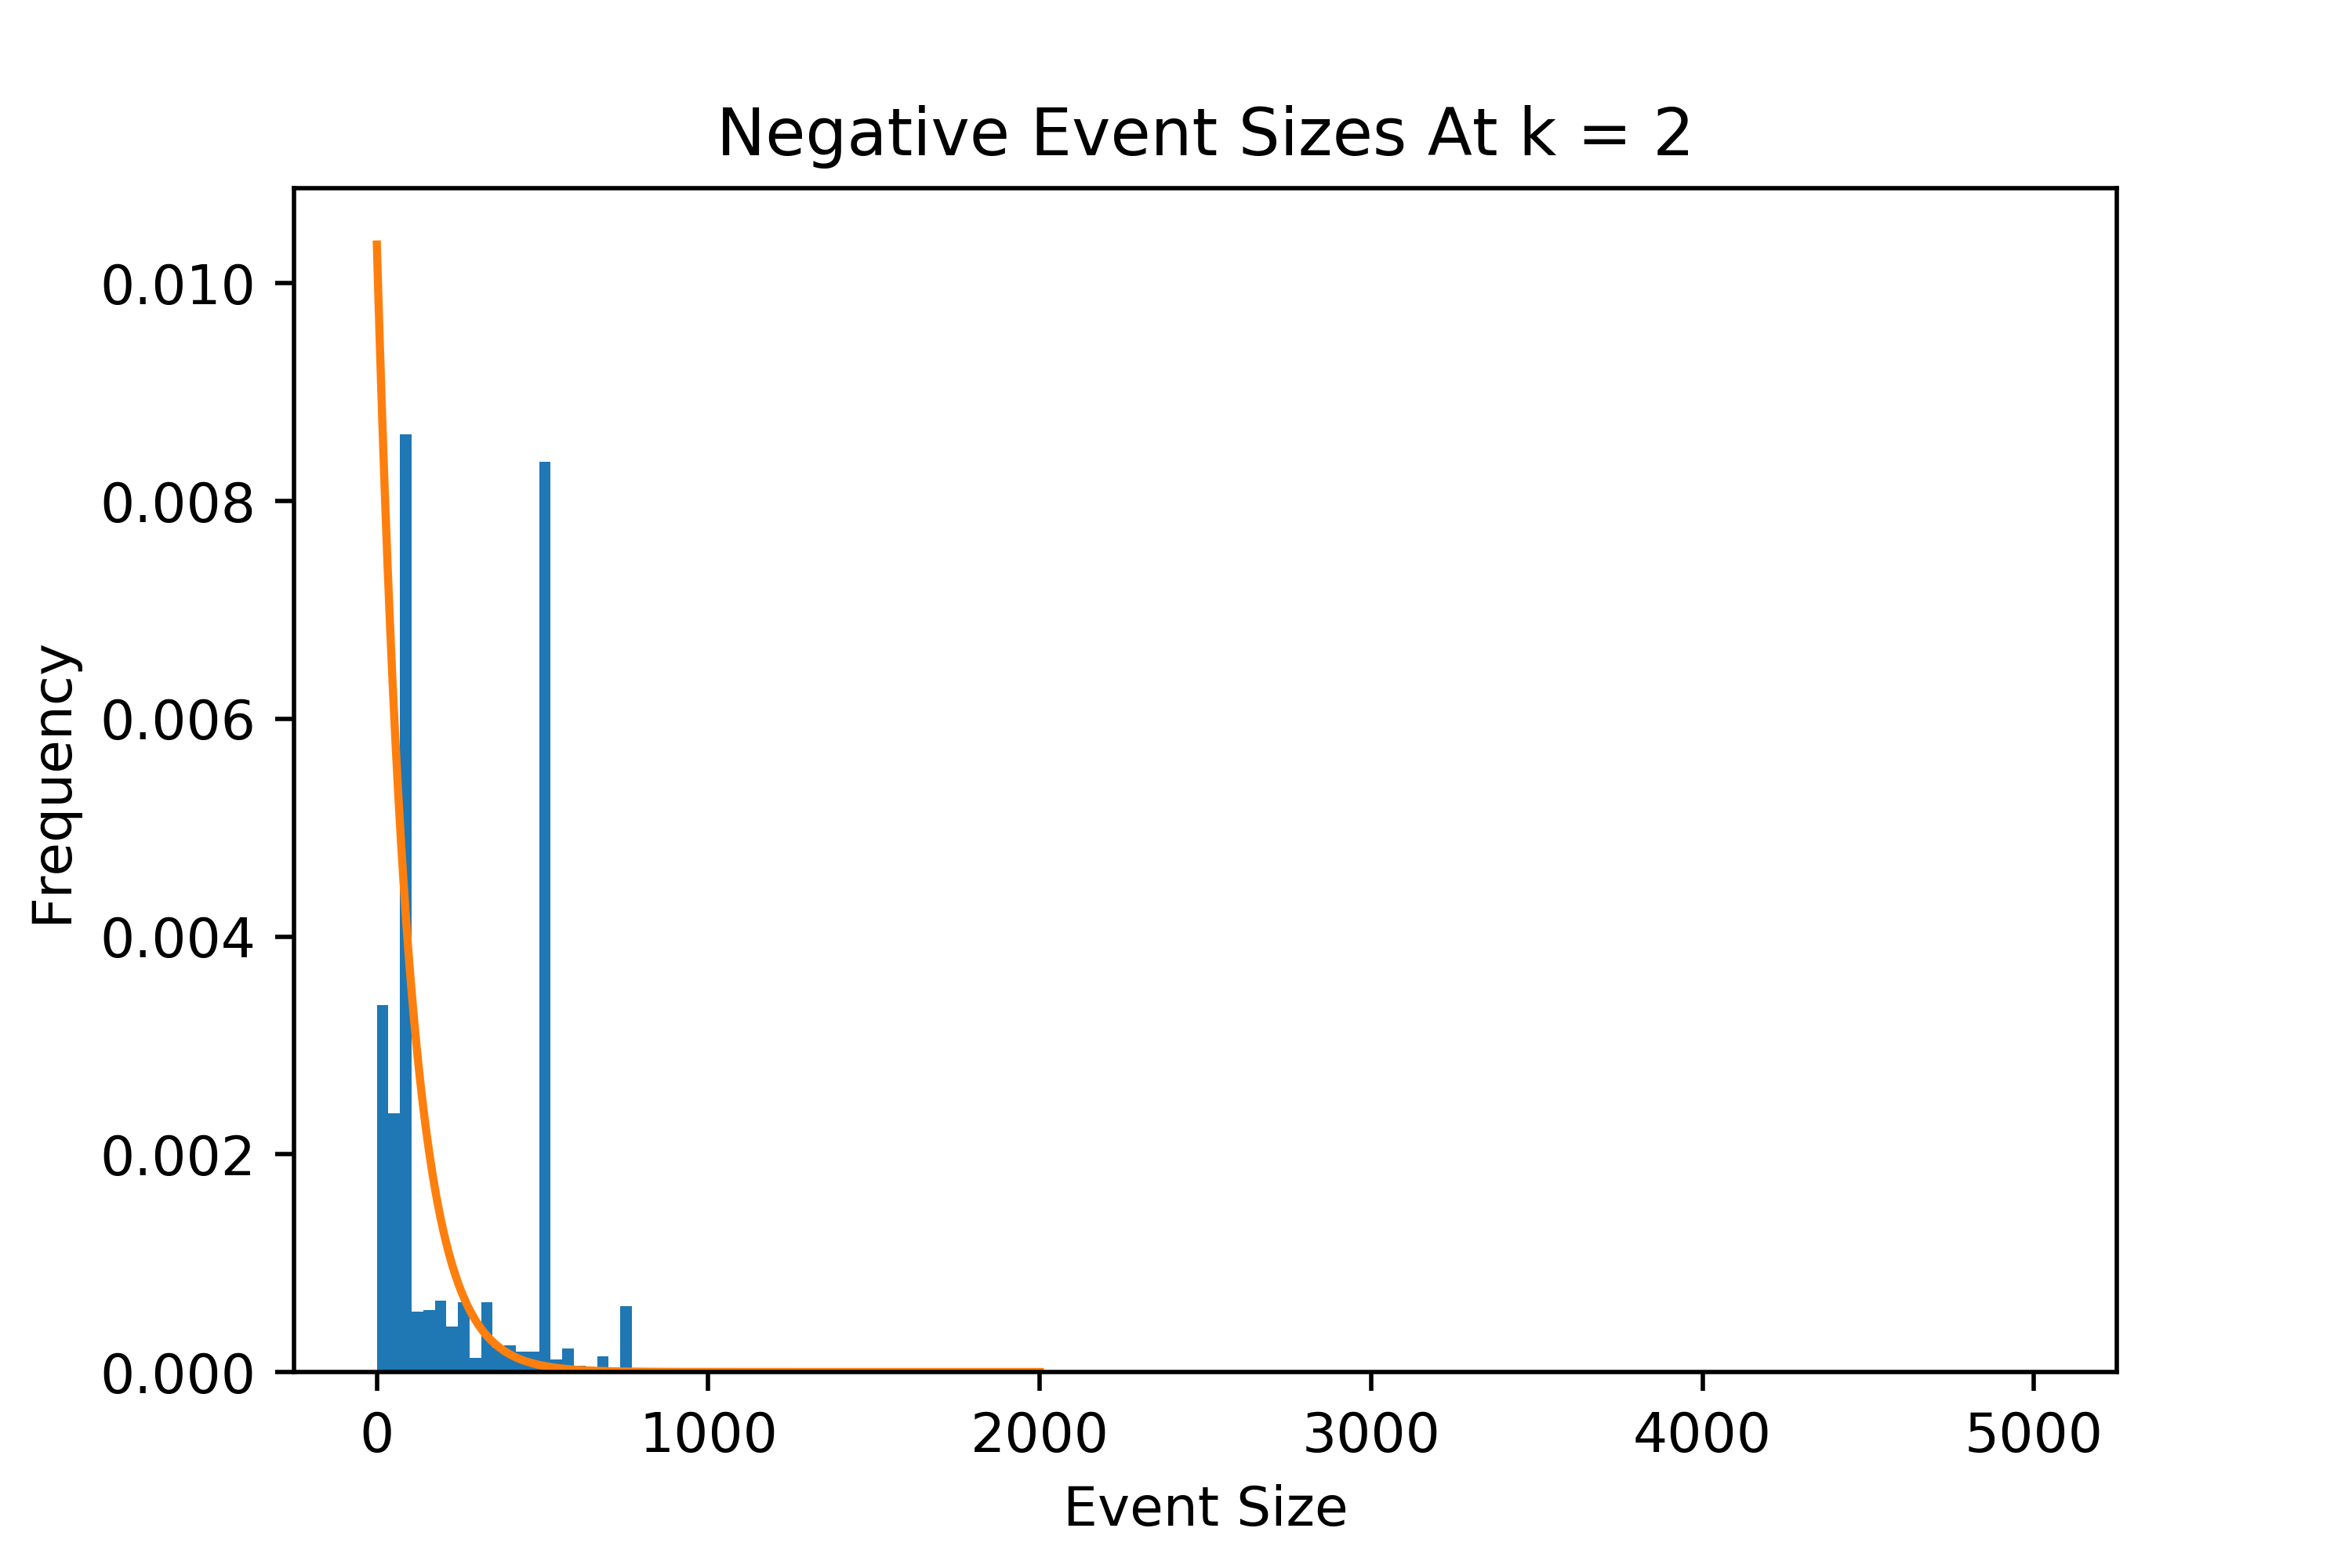
\includegraphics[width=60mm]{Figures/neg_2.png}}
% {}
% \\
\hline
\end{tabular}
\label{fig:sizes}
\end{figure}

A histogram of the event sizes along with an exponential distribution with mean equal to the $AES$ is shown in Figure \ref{fig:sizes}. As can be seen, the exponential distribution with the mean rate as the $AES$ fits the data relatively well. However, there are some notable discrepancies. One is the high frequency of orders at 500. A possible explanation for this observation is a trader splitting up a trade into equally sized amounts of size 5000. There are also a non-negligible of orders near 5000, since that is the upper limit order size imposed by Coinbase. I choose to ignore these discrepancies so that the model can be more broadly applicable, but it may be possible to more accurately model the dynamics of the ETC-USD Coinbase Pro LOB with these characteristics taken into account. The $AES$ is reported for $K=10$ in Table \ref{tab:parameters}. The code used to find the $AES$'s is found in Listing \ref{AES_and_rate_code}. It can be seen that in general, as the price gets closer to the reference price, the $AES$ decreases, but the number of events increases. This higher rate of activity around the reference price makes sense, since market orders are executed at the best available prices and market makers are incentives to provide liquidity around the reference price.

\begin{table}[htbp]
\caption{Parameter Estimates using Data from December 28-30, 2018} \label{tab:parameters}
\begin{center}
\begin{tabular}{l|llll|llll}
\hline \hline
 & \multicolumn{4}{l|}{\textbf{Positive Events}} & \multicolumn{4}{l}{\textbf{Negative Events}} \\
\hline
k   & n & $\mu^+_k$ & $\lambda^+_k$ & $\mu^+_k \lambda^+_k$ & n  & $\mu^-_k$  & $\lambda^-_k$ & $\mu^-_k \lambda^-_k$  \\
\hline
-10 & 406   & 601.41 & 0.0016 & 0.94      & 493   & 597.76 & 0.0019 & 1.14       \\
-9  & 699   & 479.69 & 0.0027 & 1.29      & 739   & 446.6  & 0.0029 & 1.27       \\
-8  & 1554  & 584.57 & 0.006  & 3.5       & 1602  & 552.68 & 0.0062 & 3.42       \\
-7  & 5633  & 530.34 & 0.0217 & 11.53     & 5417  & 534.07 & 0.0209 & 11.16      \\
-6  & 13115 & 520.95 & 0.0506 & 26.36     & 12852 & 531.86 & 0.0496 & 26.37      \\
-5  & 21824 & 487.88 & 0.0842 & 41.08     & 21850 & 494.66 & 0.0843 & 41.7       \\
-4  & 27620 & 427.19 & 0.1066 & 45.52     & 27578 & 433.09 & 0.1064 & 46.08      \\
-3  & 33187 & 368.47 & 0.128  & 47.18     & 33214 & 367.8  & 0.1281 & 47.13      \\
-2  & 47229 & 232.15 & 0.1822 & 42.3      & 45189 & 247.63 & 0.1743 & 43.17      \\
-1  & 54254 & 104.11 & 0.2093 & 21.79     & 49177 & 104.8  & 0.1897 & 19.88      \\
1   & 48246 & 93.79  & 0.1861 & 17.46     & 46787 & 89.82  & 0.1805 & 16.21      \\
2   & 37702 & 226.64 & 0.1455 & 32.96     & 38310 & 229.59 & 0.1478 & 33.93      \\
3   & 41409 & 305.04 & 0.1598 & 48.73     & 41912 & 302.37 & 0.1617 & 48.89      \\
4   & 44948 & 328.57 & 0.1734 & 56.98     & 44616 & 333.46 & 0.1721 & 57.4       \\
5   & 37880 & 318.37 & 0.1461 & 46.53     & 37105 & 325.12 & 0.1431 & 46.54      \\
6   & 16320 & 360.54 & 0.063  & 22.7      & 15669 & 375.32 & 0.0604 & 22.69      \\
7   & 3818  & 577.4  & 0.0147 & 8.5       & 3672  & 587.94 & 0.0142 & 8.33       \\
8   & 1271  & 599.09 & 0.0049 & 2.94      & 1280  & 516.85 & 0.0049 & 2.55       \\
9   & 602   & 428.87 & 0.0023 & 1         & 543   & 484.68 & 0.0021 & 1.02       \\
10  & 548   & 366.15 & 0.0021 & 0.77      & 529   & 370.48 & 0.002  & 0.76      
\end{tabular}
\end{center}
\end{table}

\section{Arrival Rate Estimates}\label{ch:poisson}
We model the event arrivals as a multivariate Poisson process, where the marginal processes at each position $k$ have average arrival rates $\lambda^+_k$ and $\lambda^-_k$. We examine whether individual event arrivals at each position can be modelled as a Poisson process. To do so, I test whether the inter-arrival times of the events are exponentially distributed. Figures \ref{fig:interarrivals_pos} and \ref{fig:interarrivals_neg} show QQ-plots and histograms of the inter-arrival times compared to an exponential distribution. From the QQ-plots, it can be seen from the QQ-plots have heavy right tails compared to the exponential distribution. It can be seen from the histograms that the exponential distribution fits the data well for the majority of the points except for a small number of outliers to the right (the heavy tails). Despite this discrepancy, I choose to model the arrivals as a Poisson process because the number of outliers is small and for the Poisson processes' desirable properties in simulation. We  estimate $\lambda^+_k$ and $\lambda^-_k$ by taking number of arrivals of the specified event divided by the total time period. The code used to find the the rates is found in Listing \ref{AES_and_rate_code}. The average rates $\lambda^+_k$ and $\lambda^-_k$ for $K=10$ are reported in Table \ref{tab:parameters}.

\begin{figure}
\centering
\caption{Inter-Arrival Times Compared to Exponential Distribution using Data from December 28-30, 2018}
\begin{tabular}{cc}
\hline
\subf{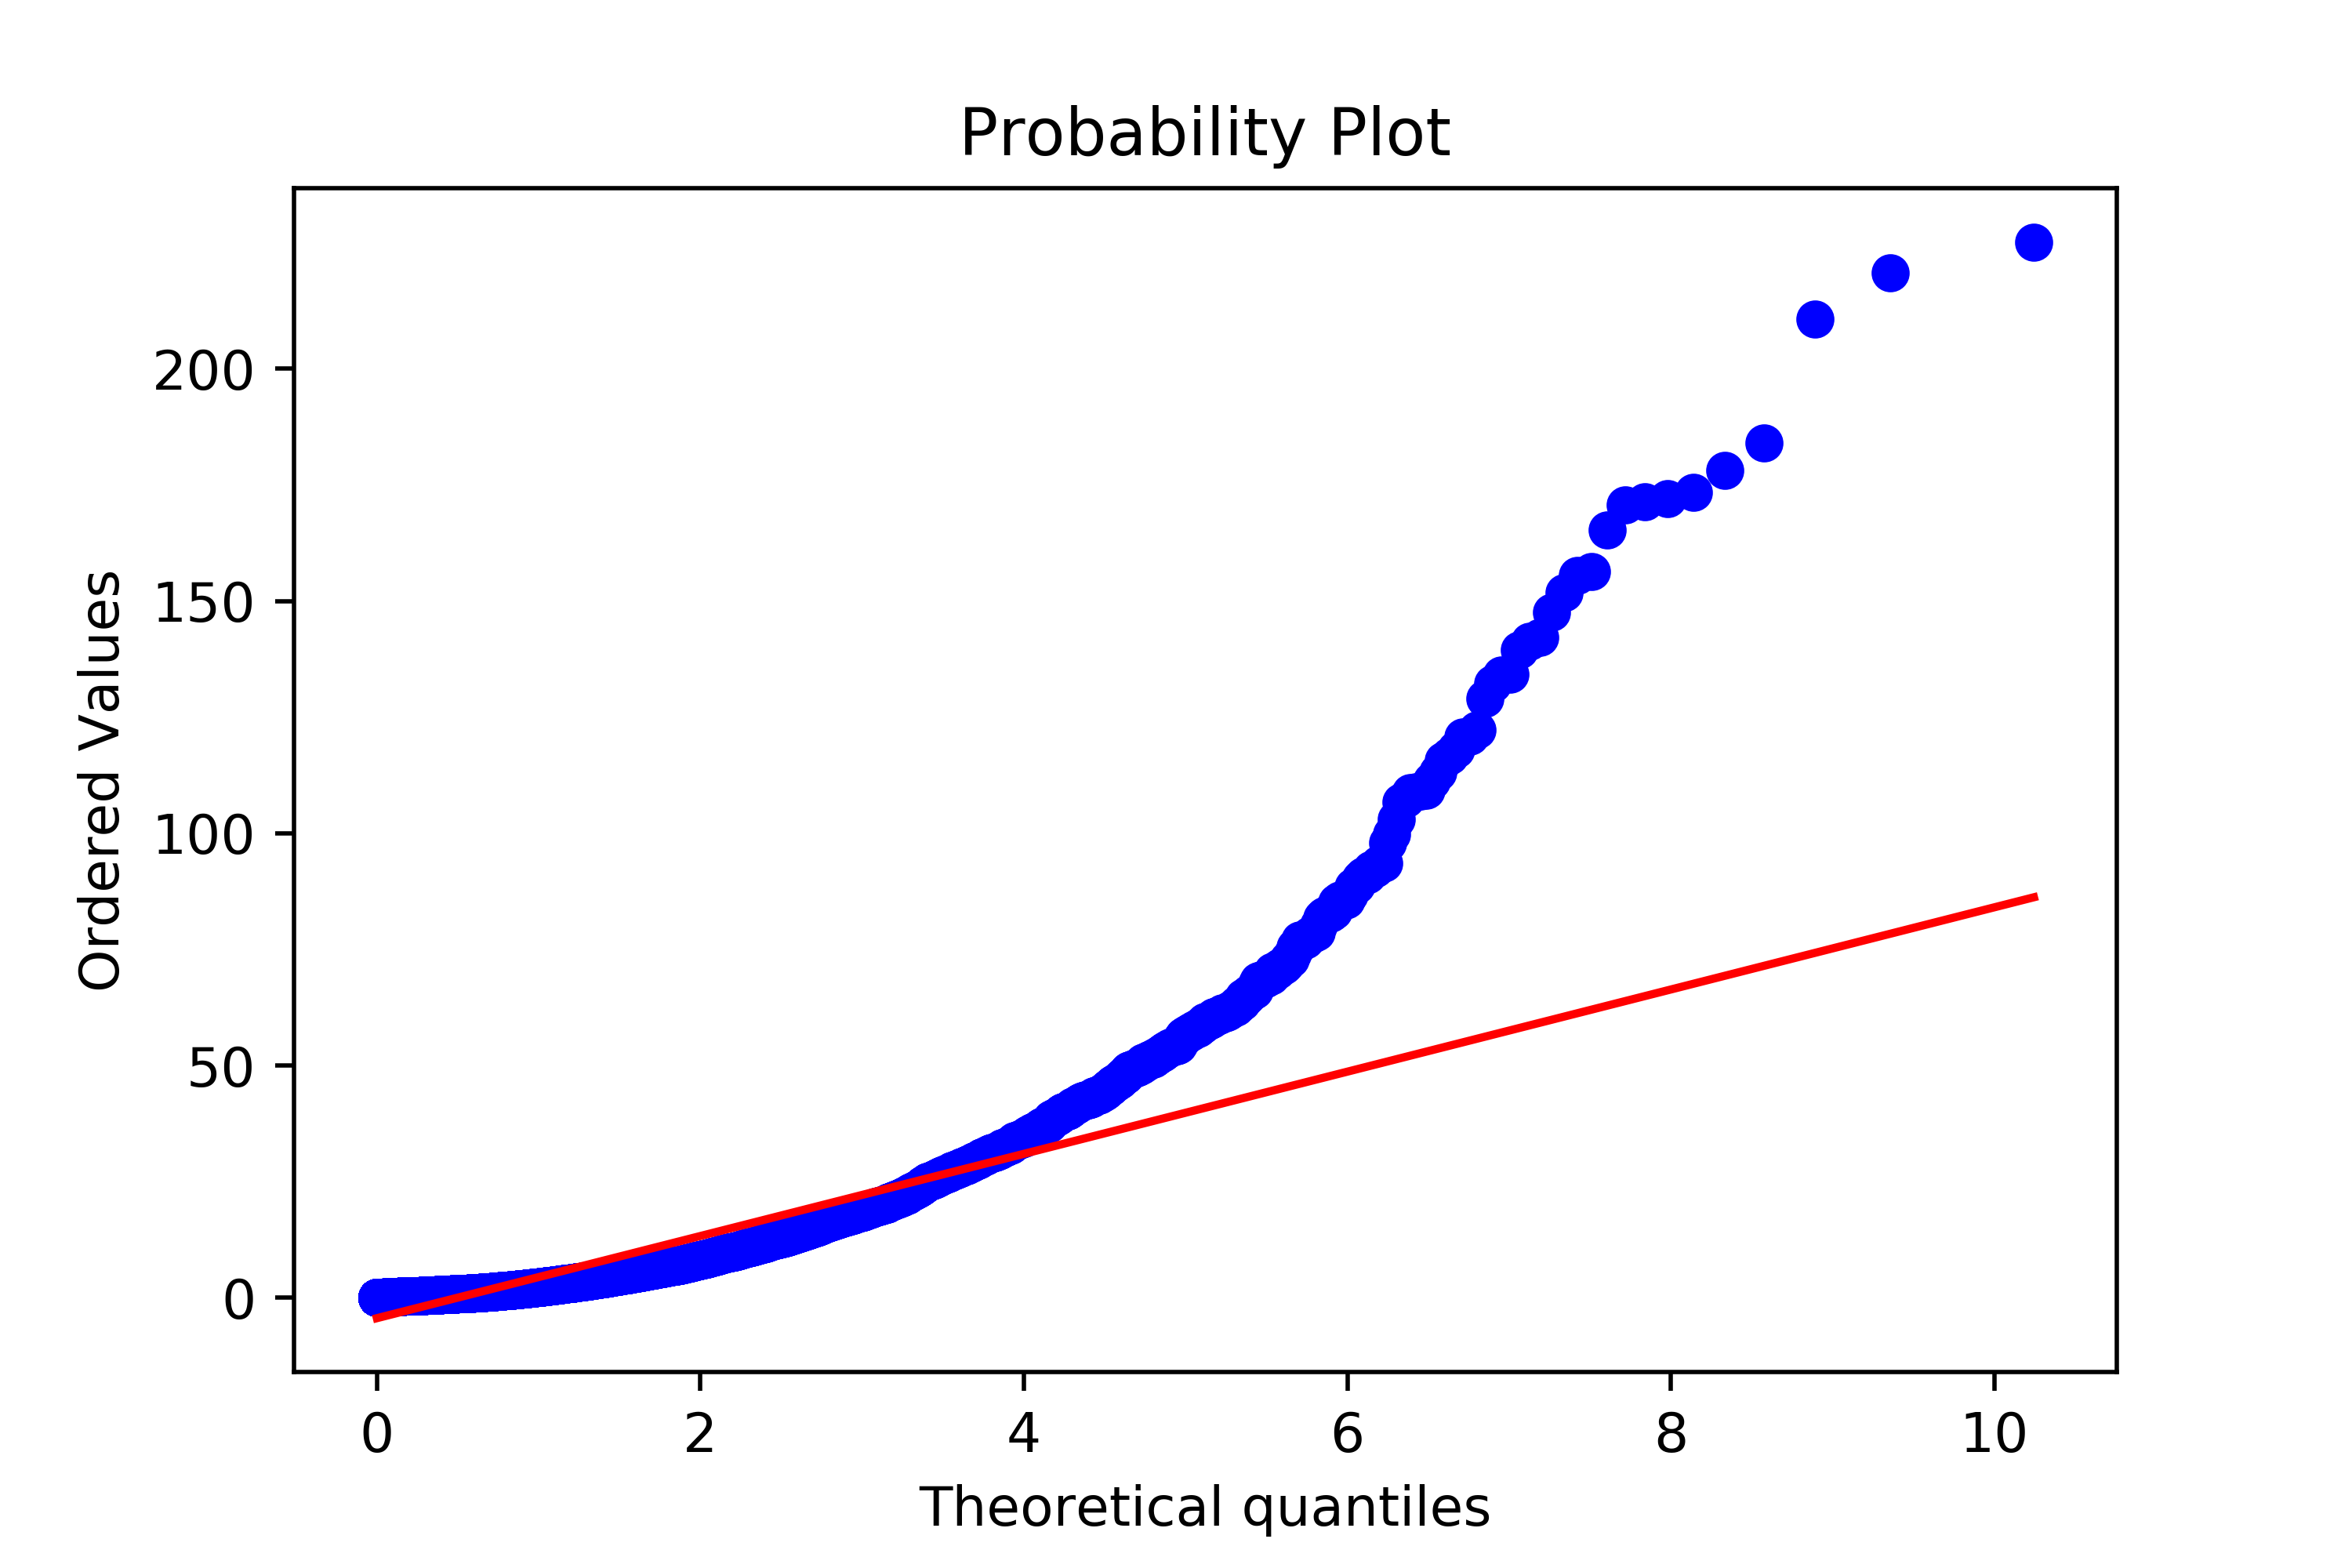
\includegraphics[width=60mm]{Figures/QQ_pos_k-2.png}}
{}
&
\subf{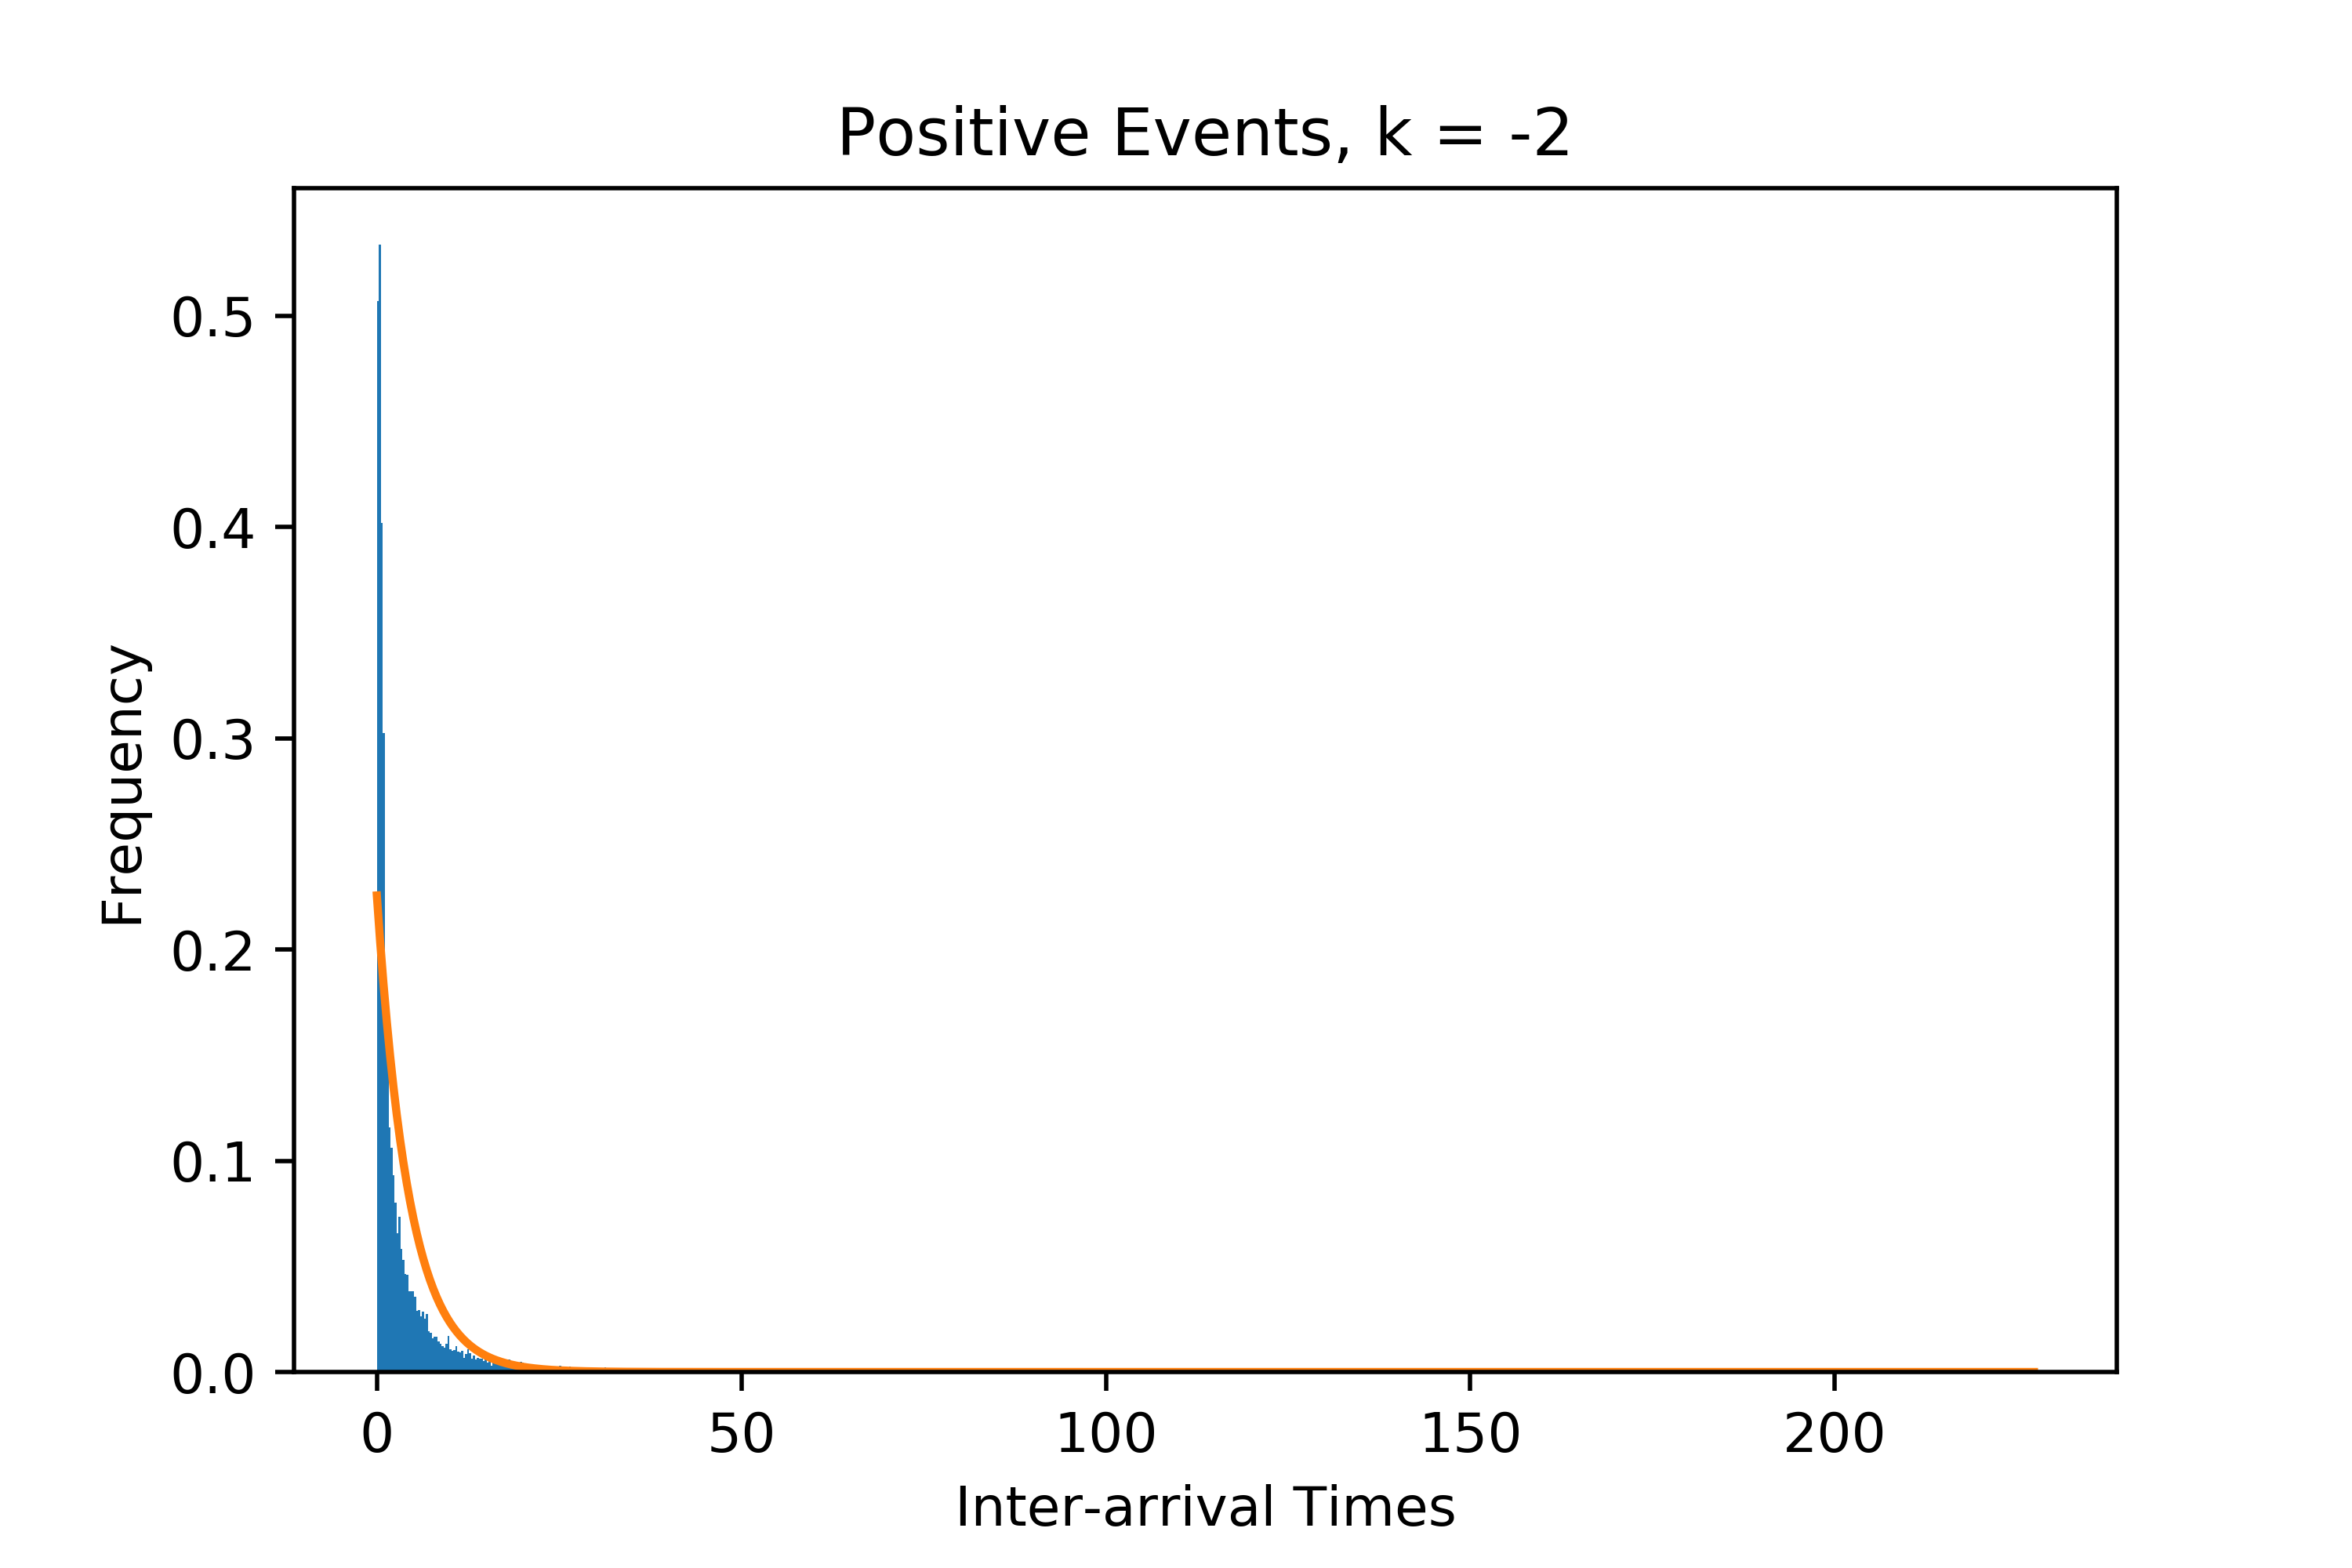
\includegraphics[width=60mm]{Figures/hist_pos_k-2.png}}
{}
\\
\subf{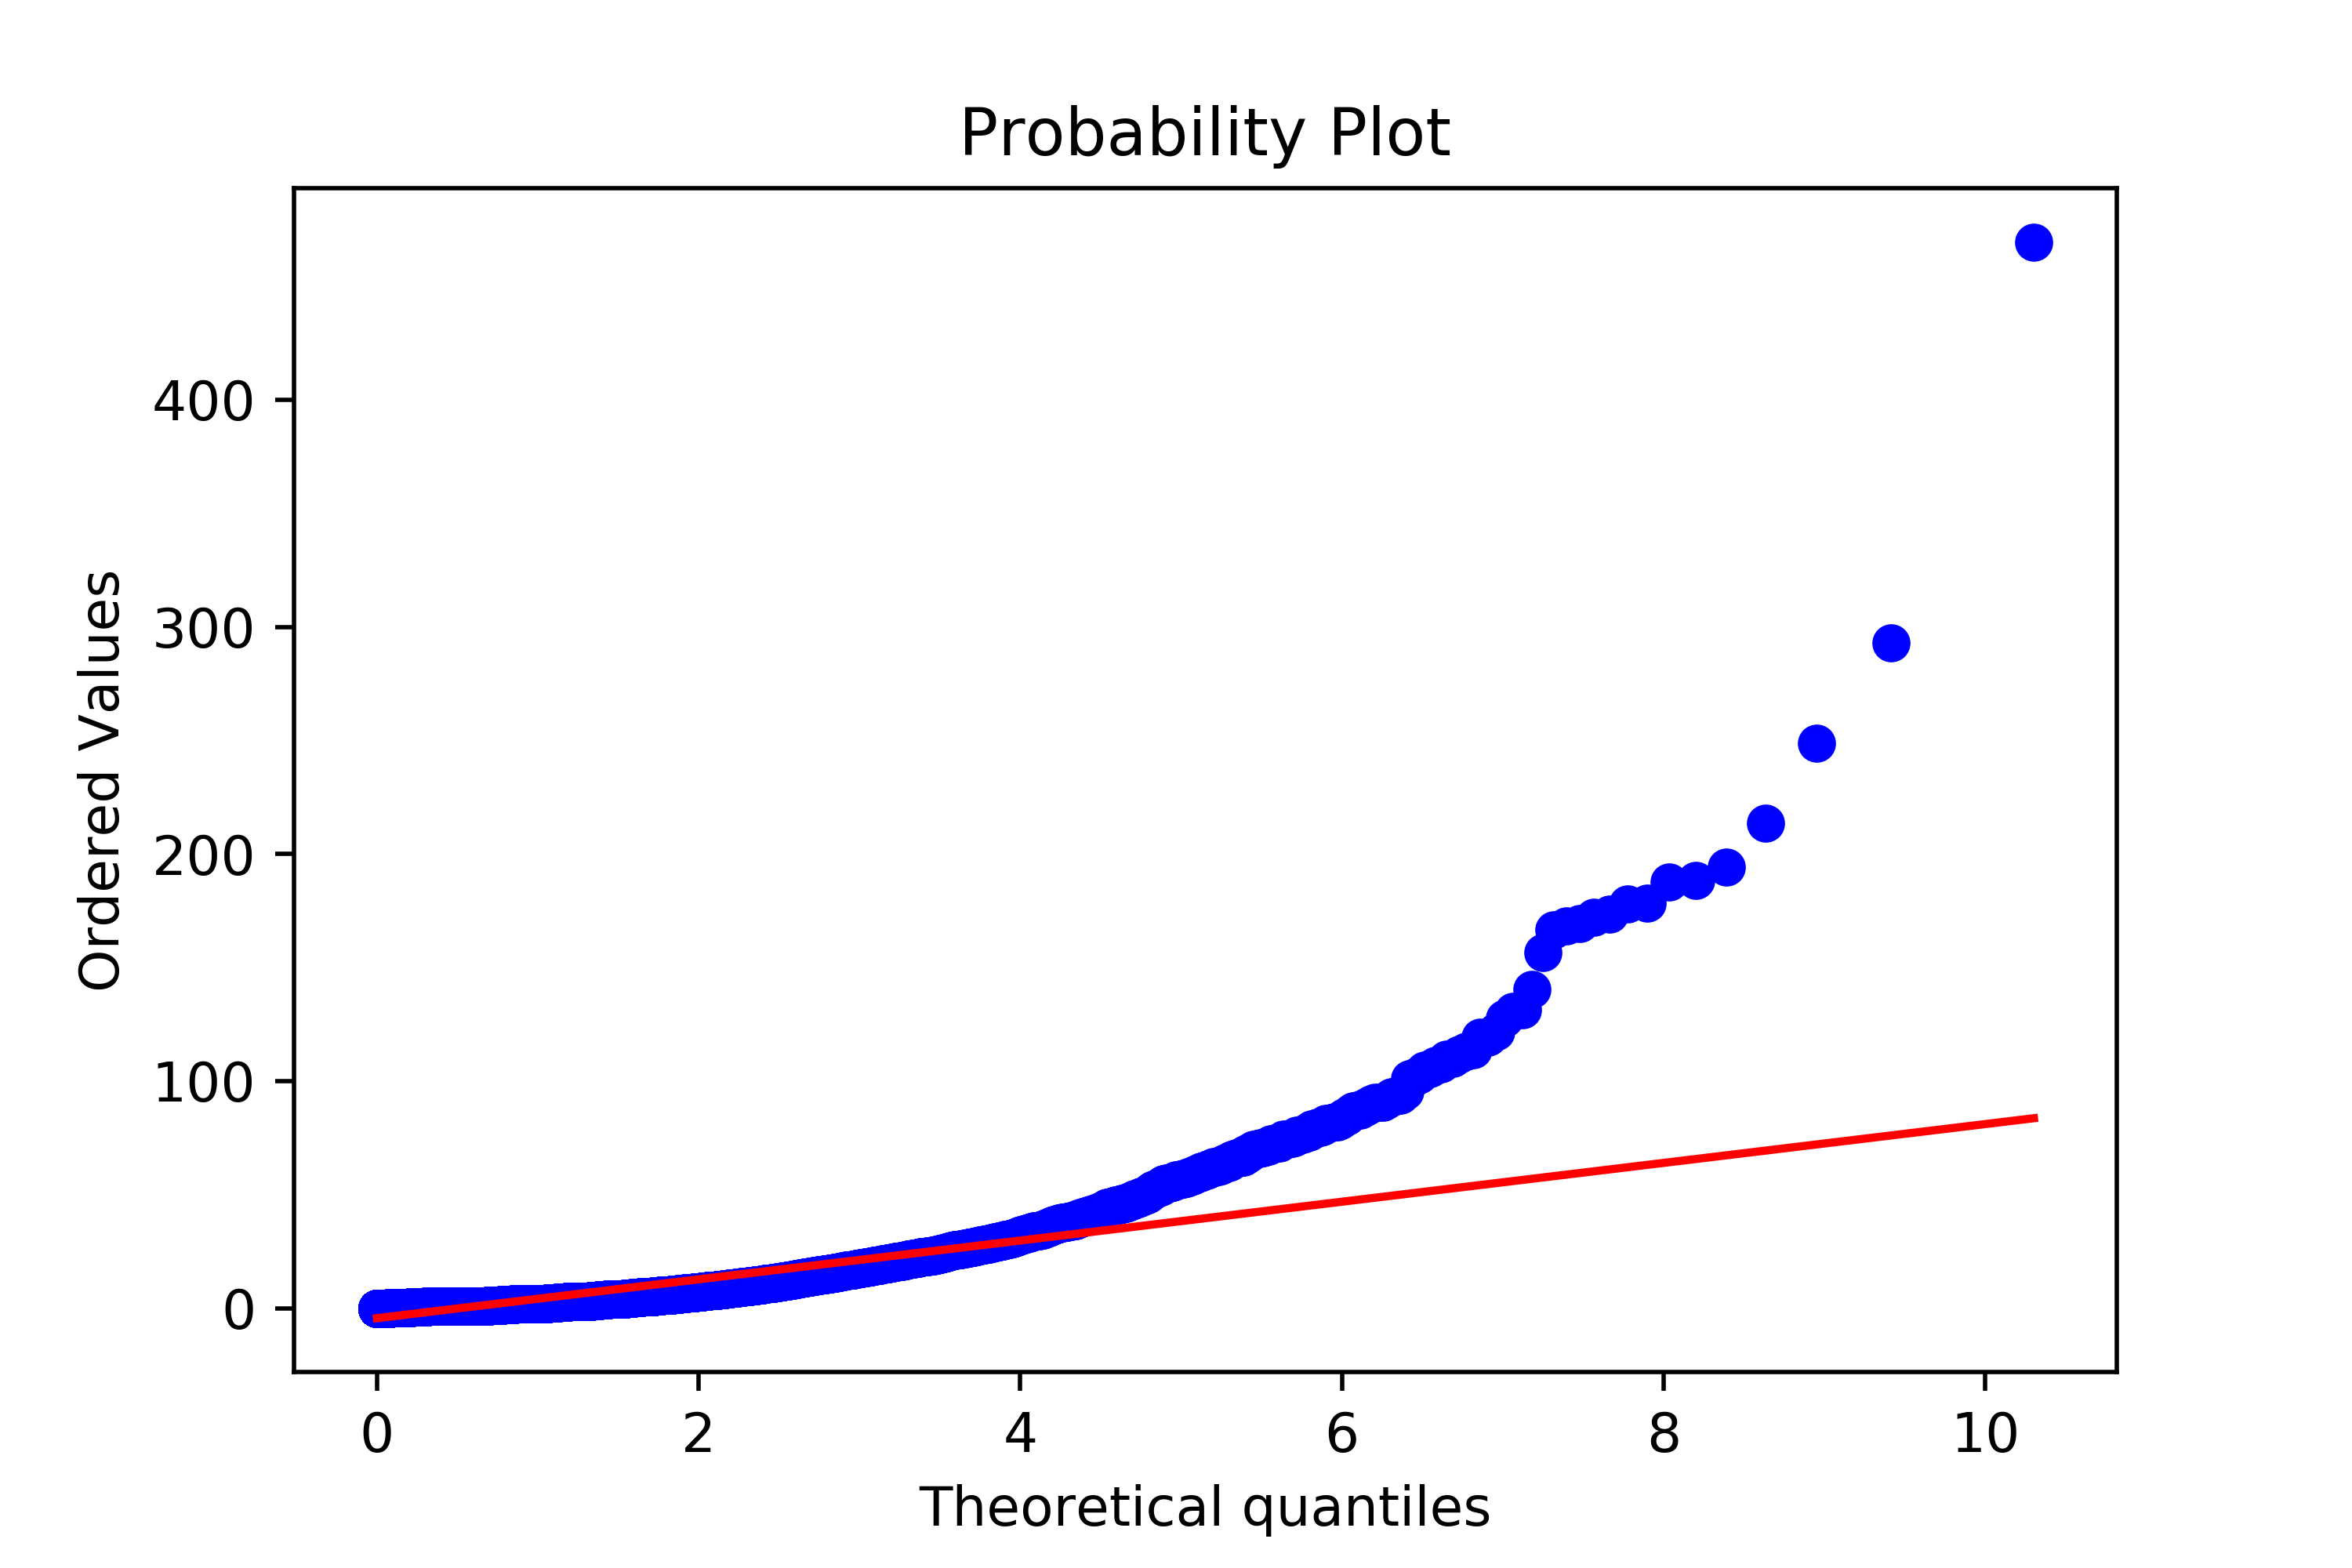
\includegraphics[width=60mm]{Figures/QQ_pos_k-1.png}}
{}
&
\subf{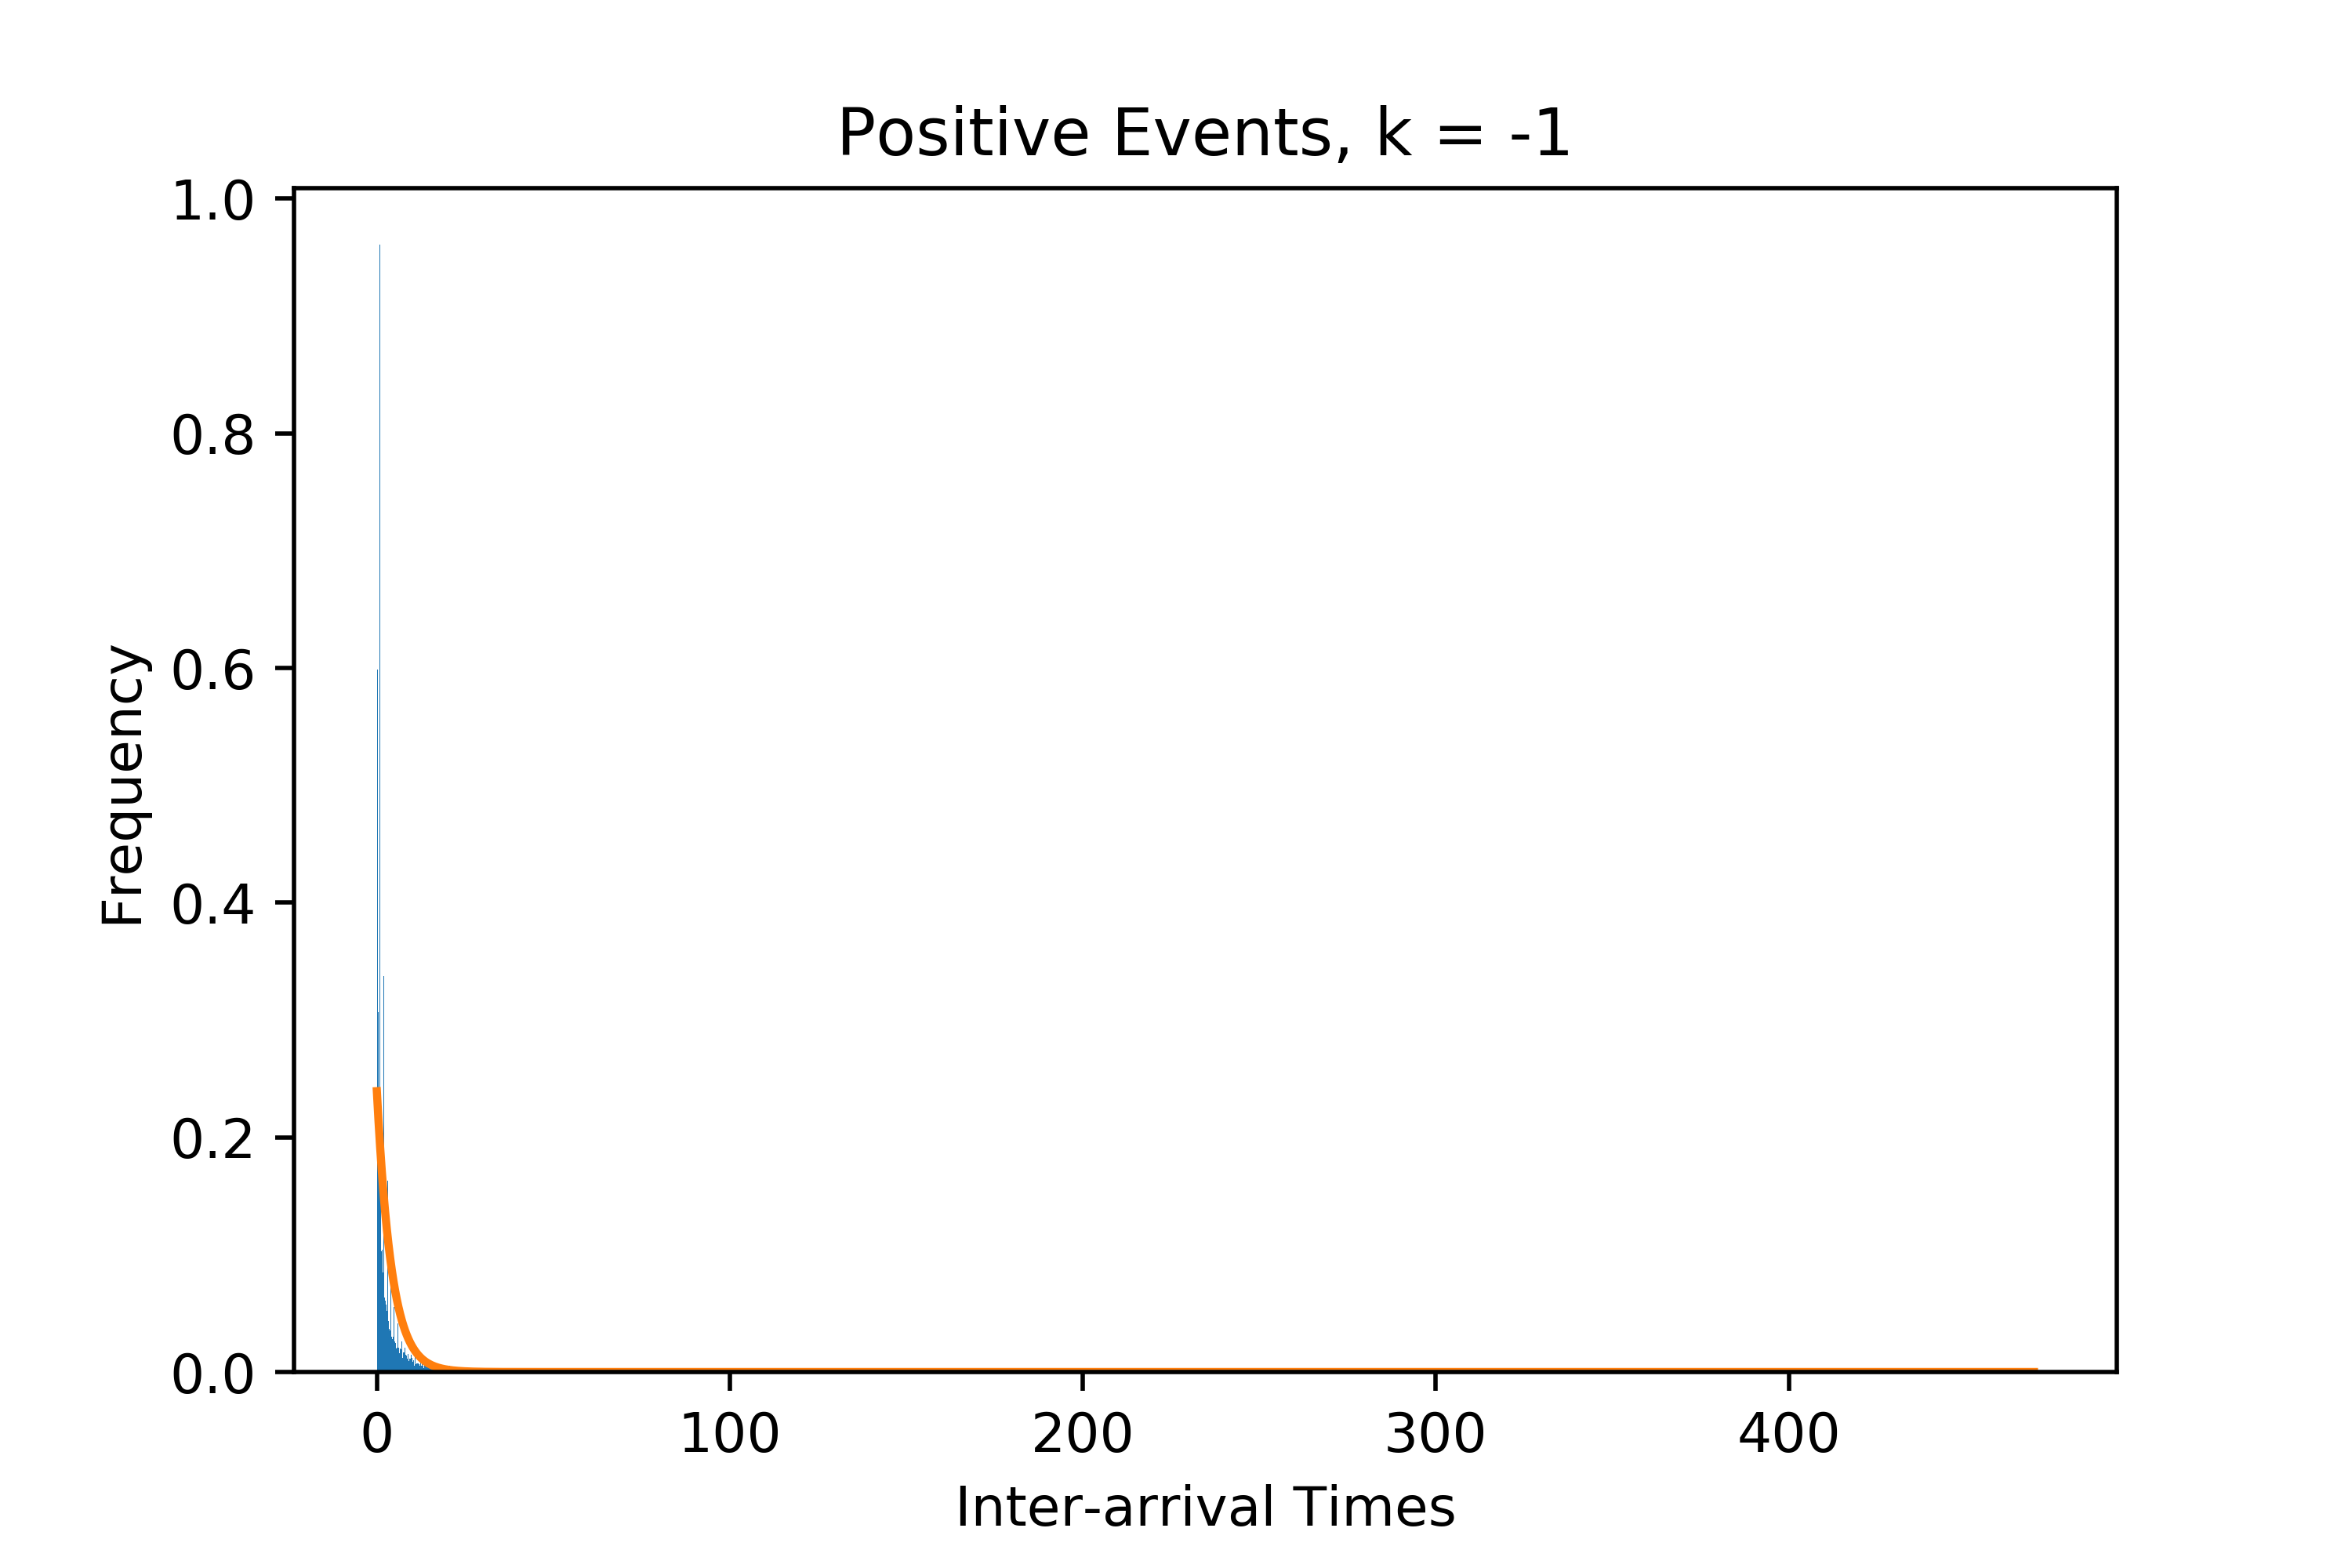
\includegraphics[width=60mm]{Figures/hist_pos_k-1.png}}
{}
\\
\subf{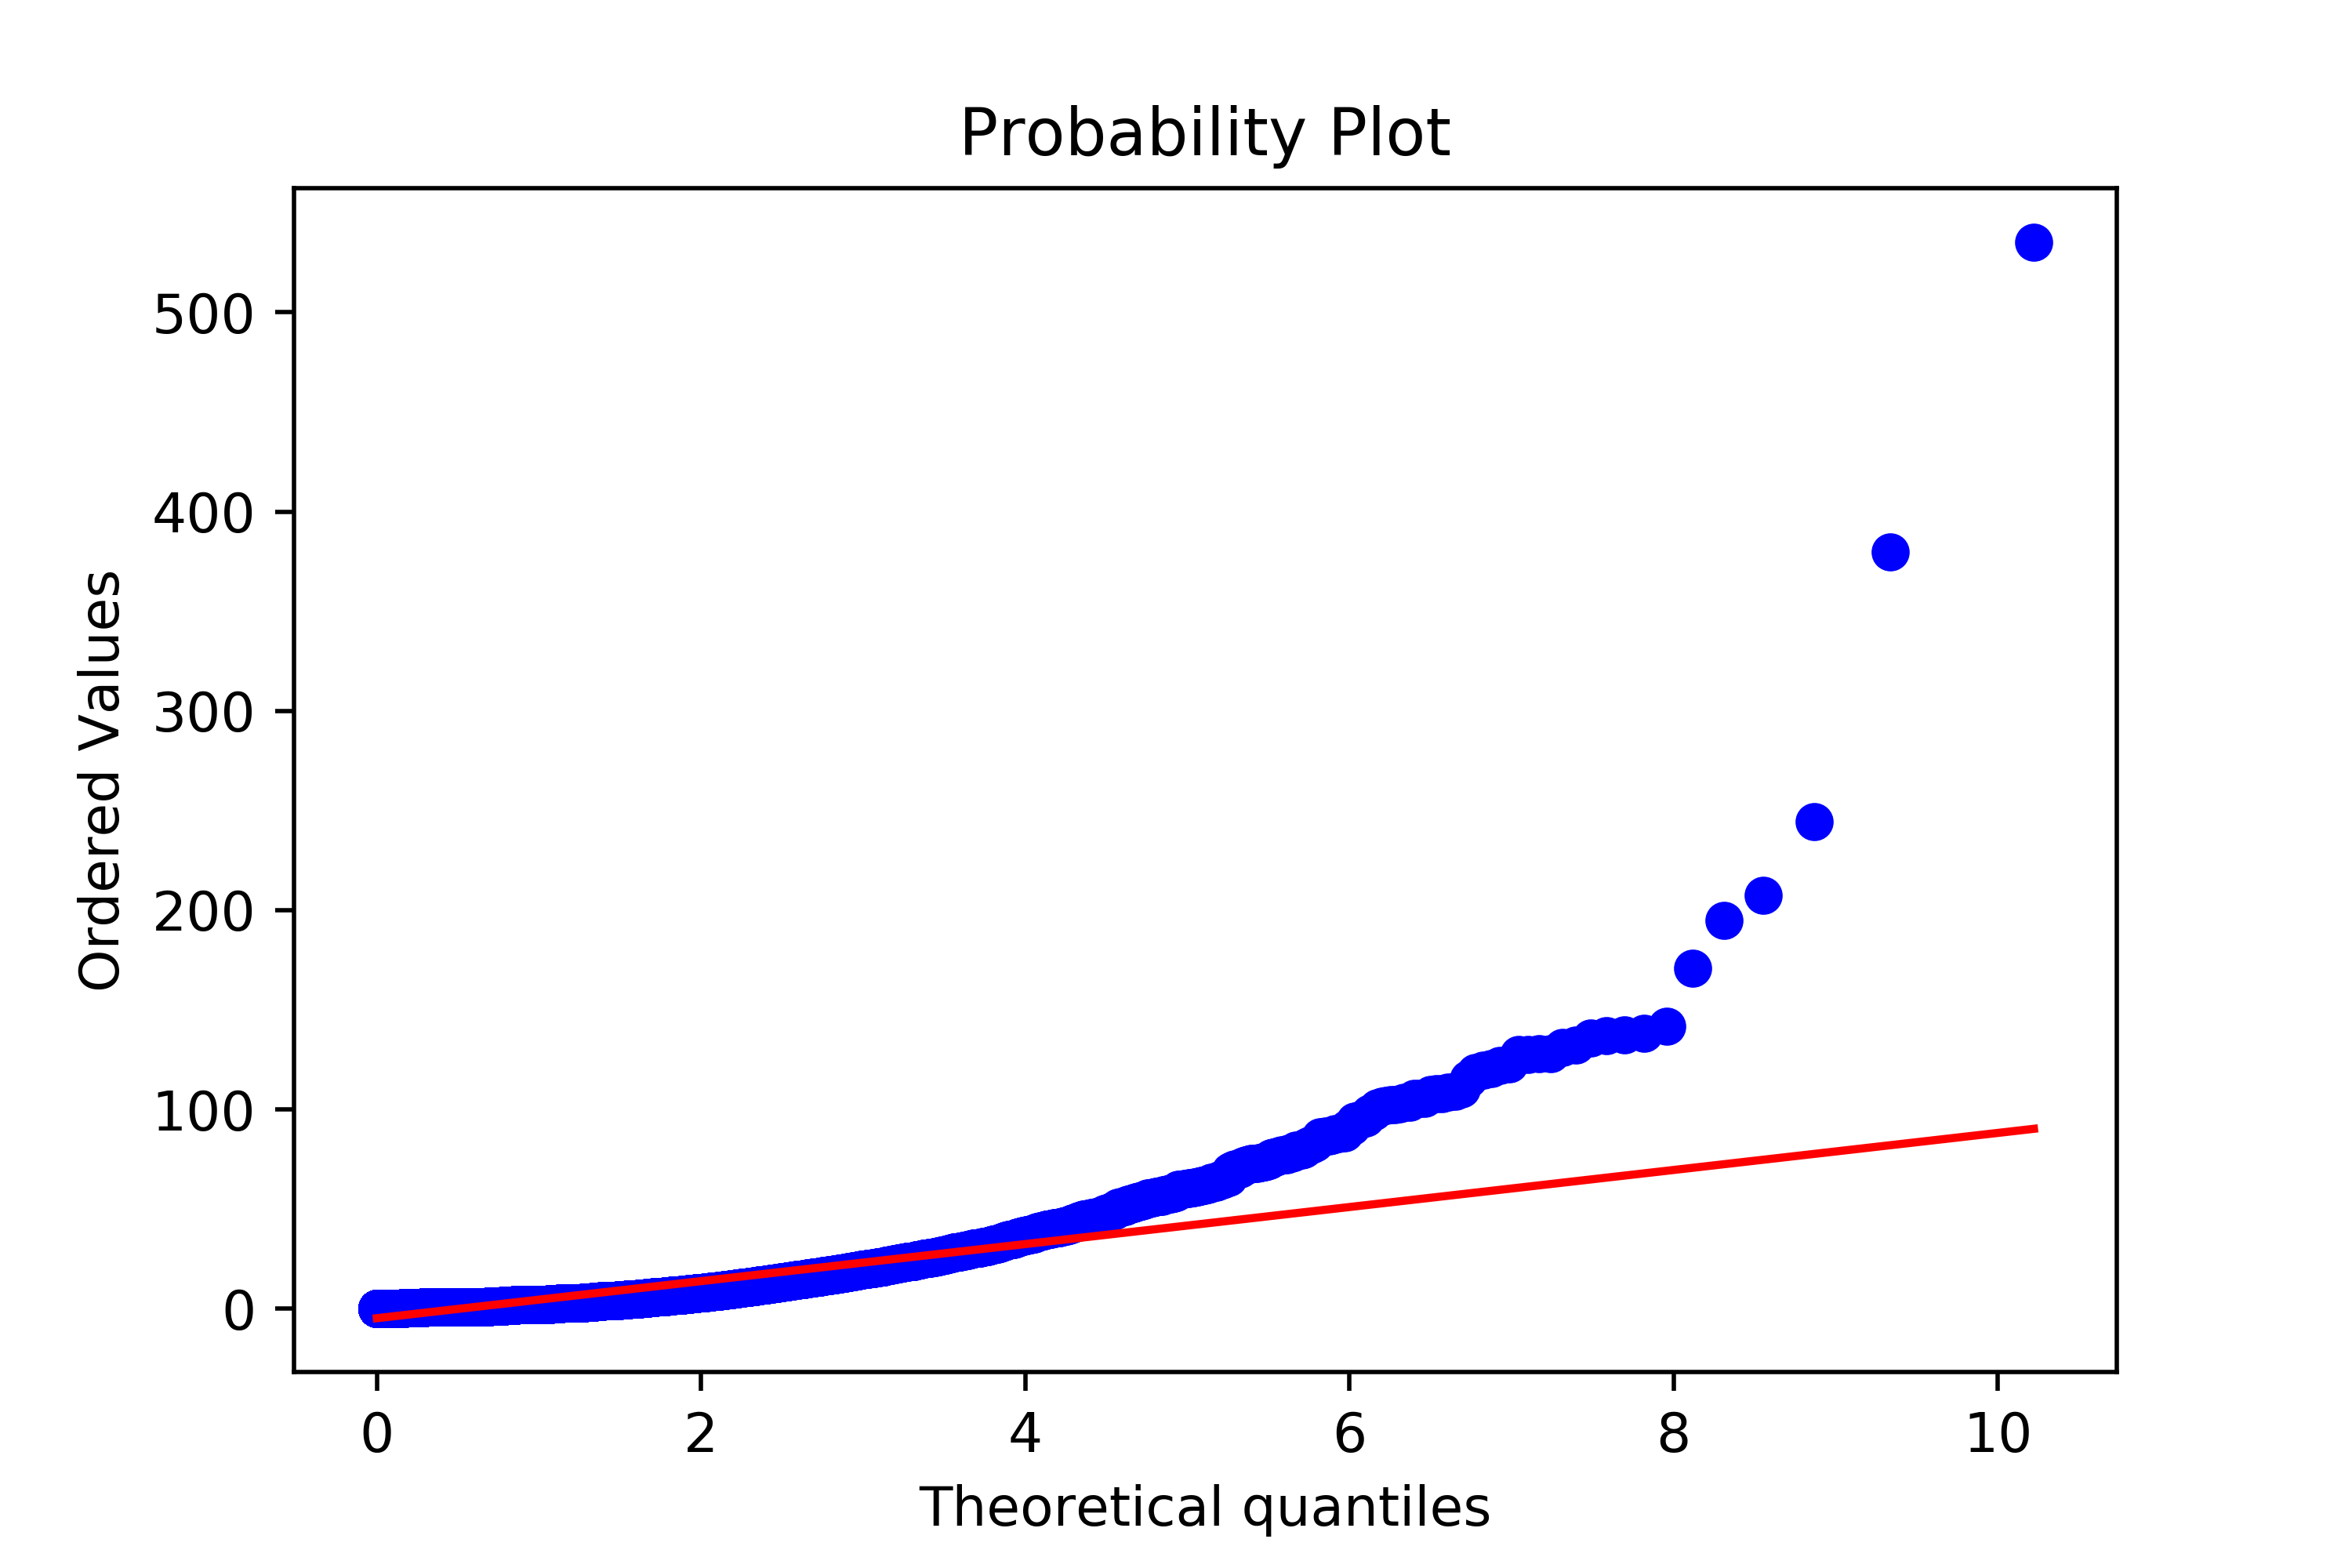
\includegraphics[width=60mm]{Figures/QQ_pos_k1.png}}
{}
&
\subf{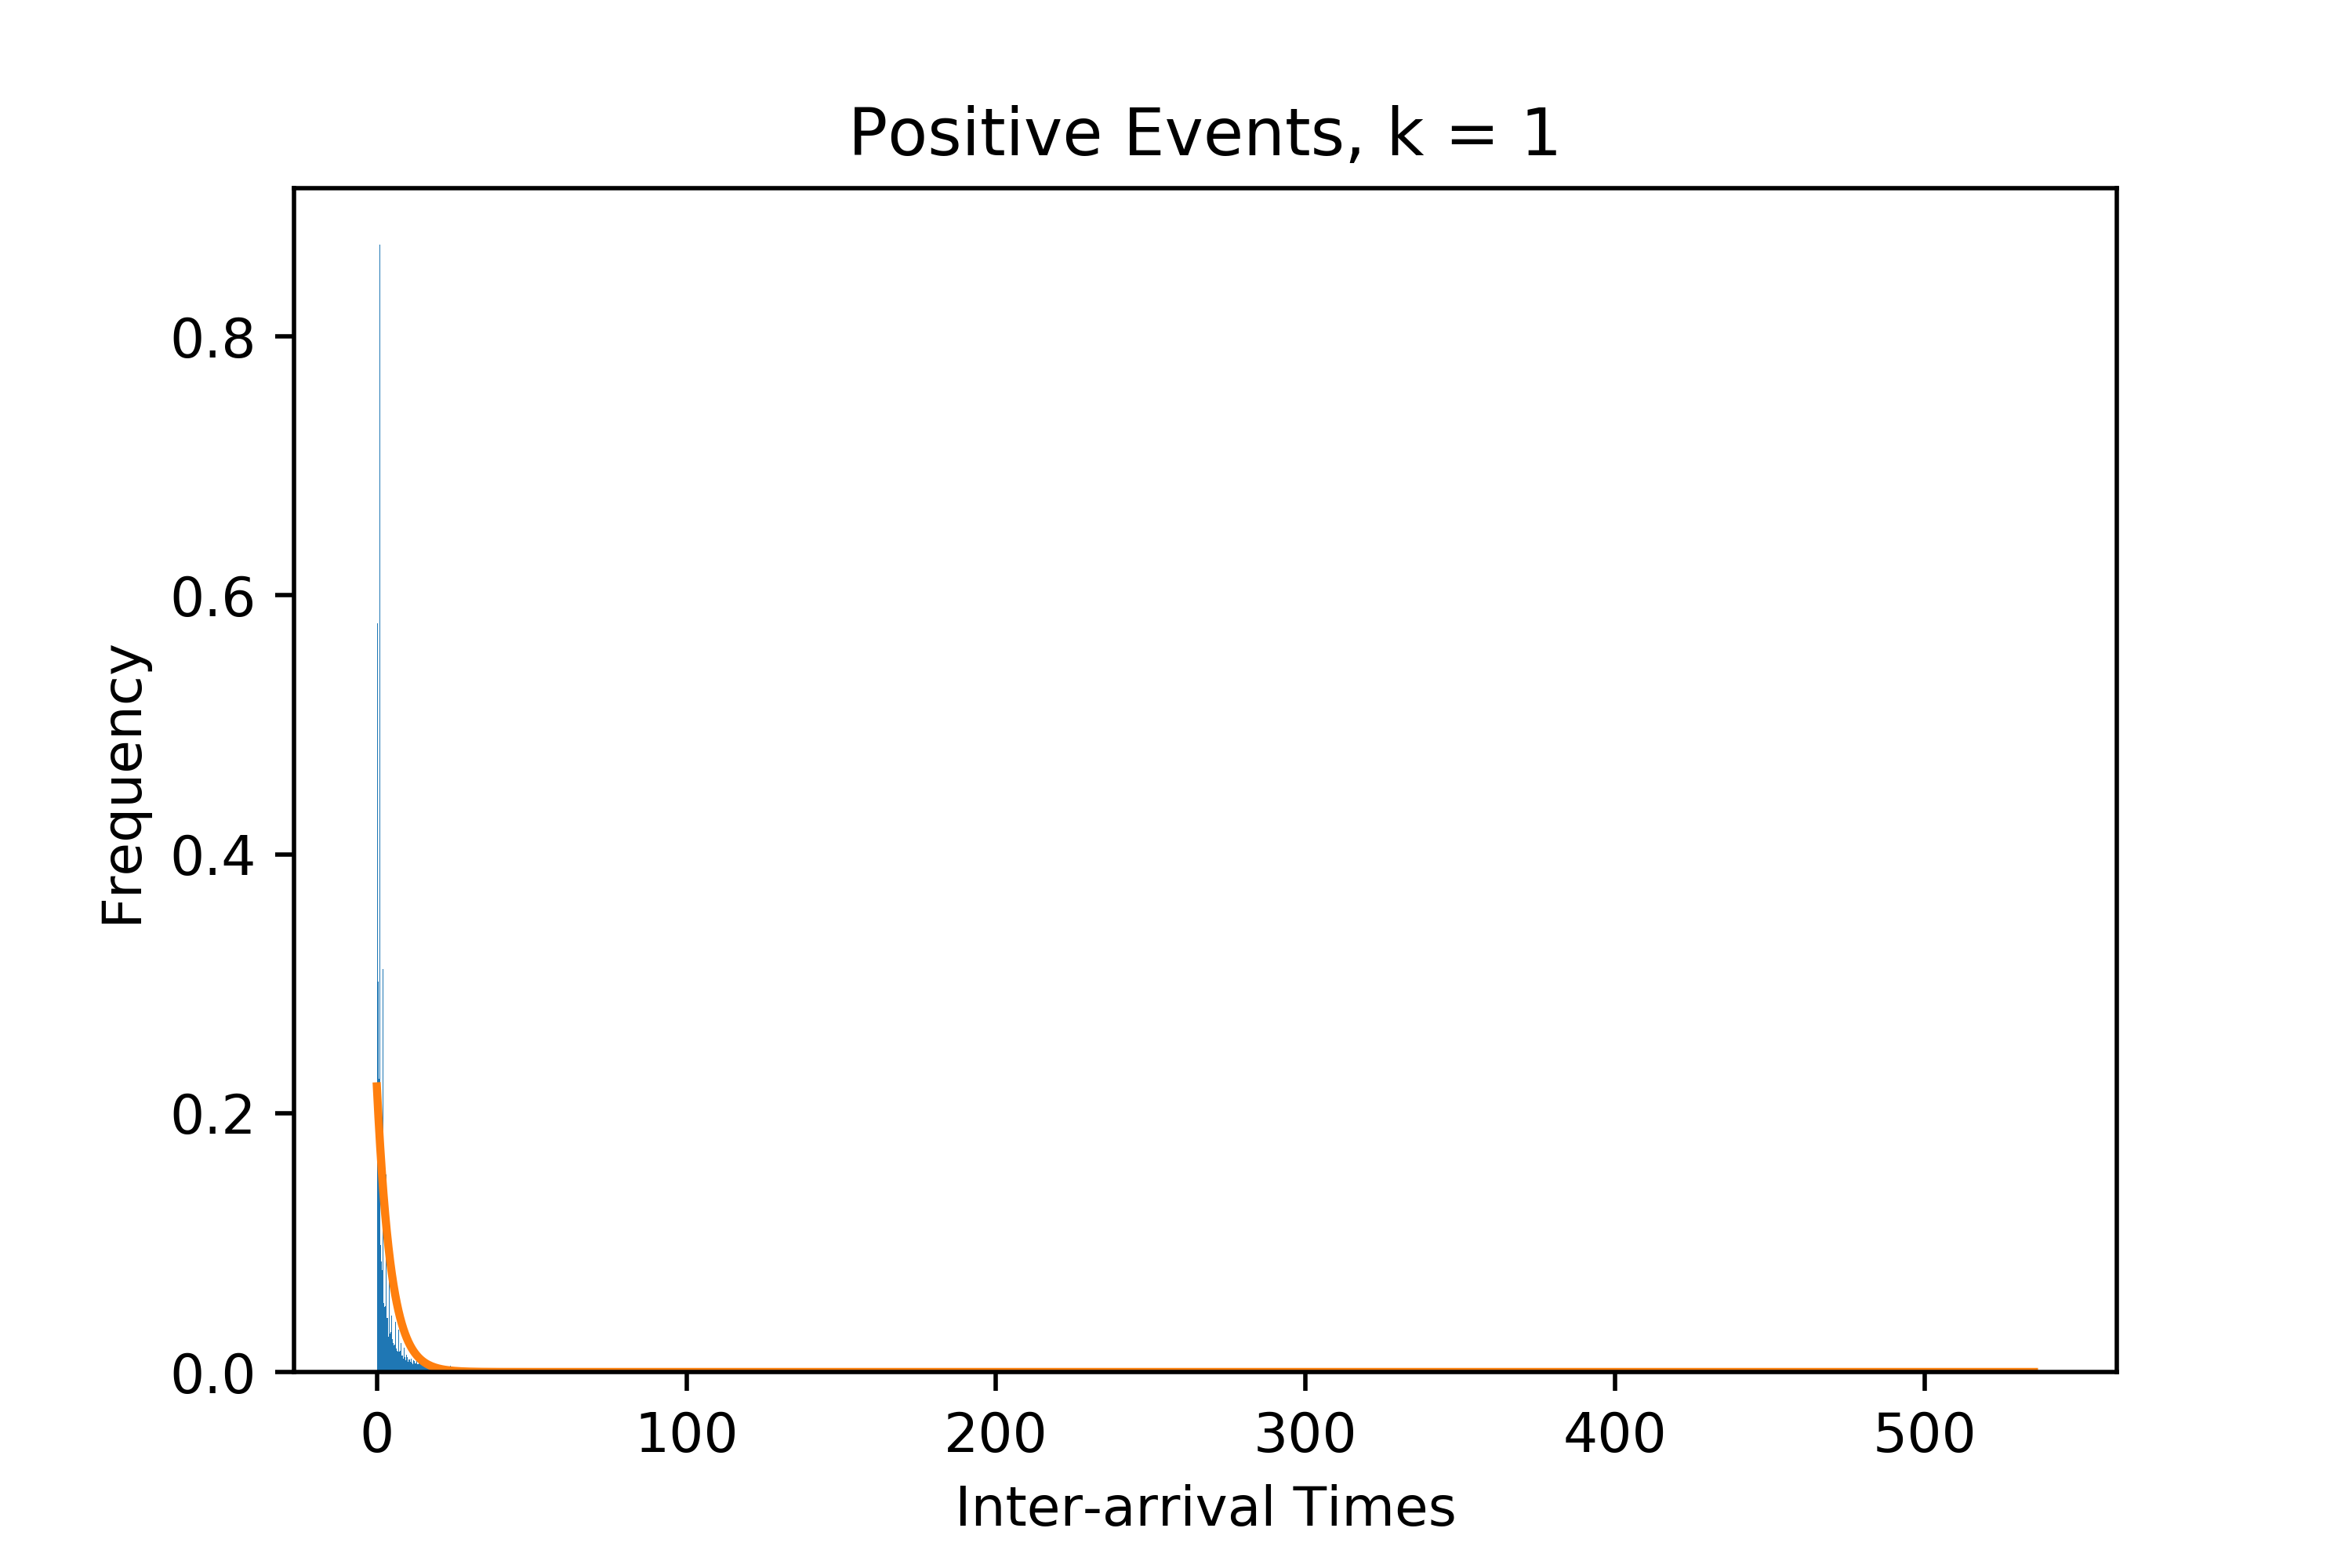
\includegraphics[width=60mm]{Figures/hist_pos_k1.png}}
{}
\\
\subf{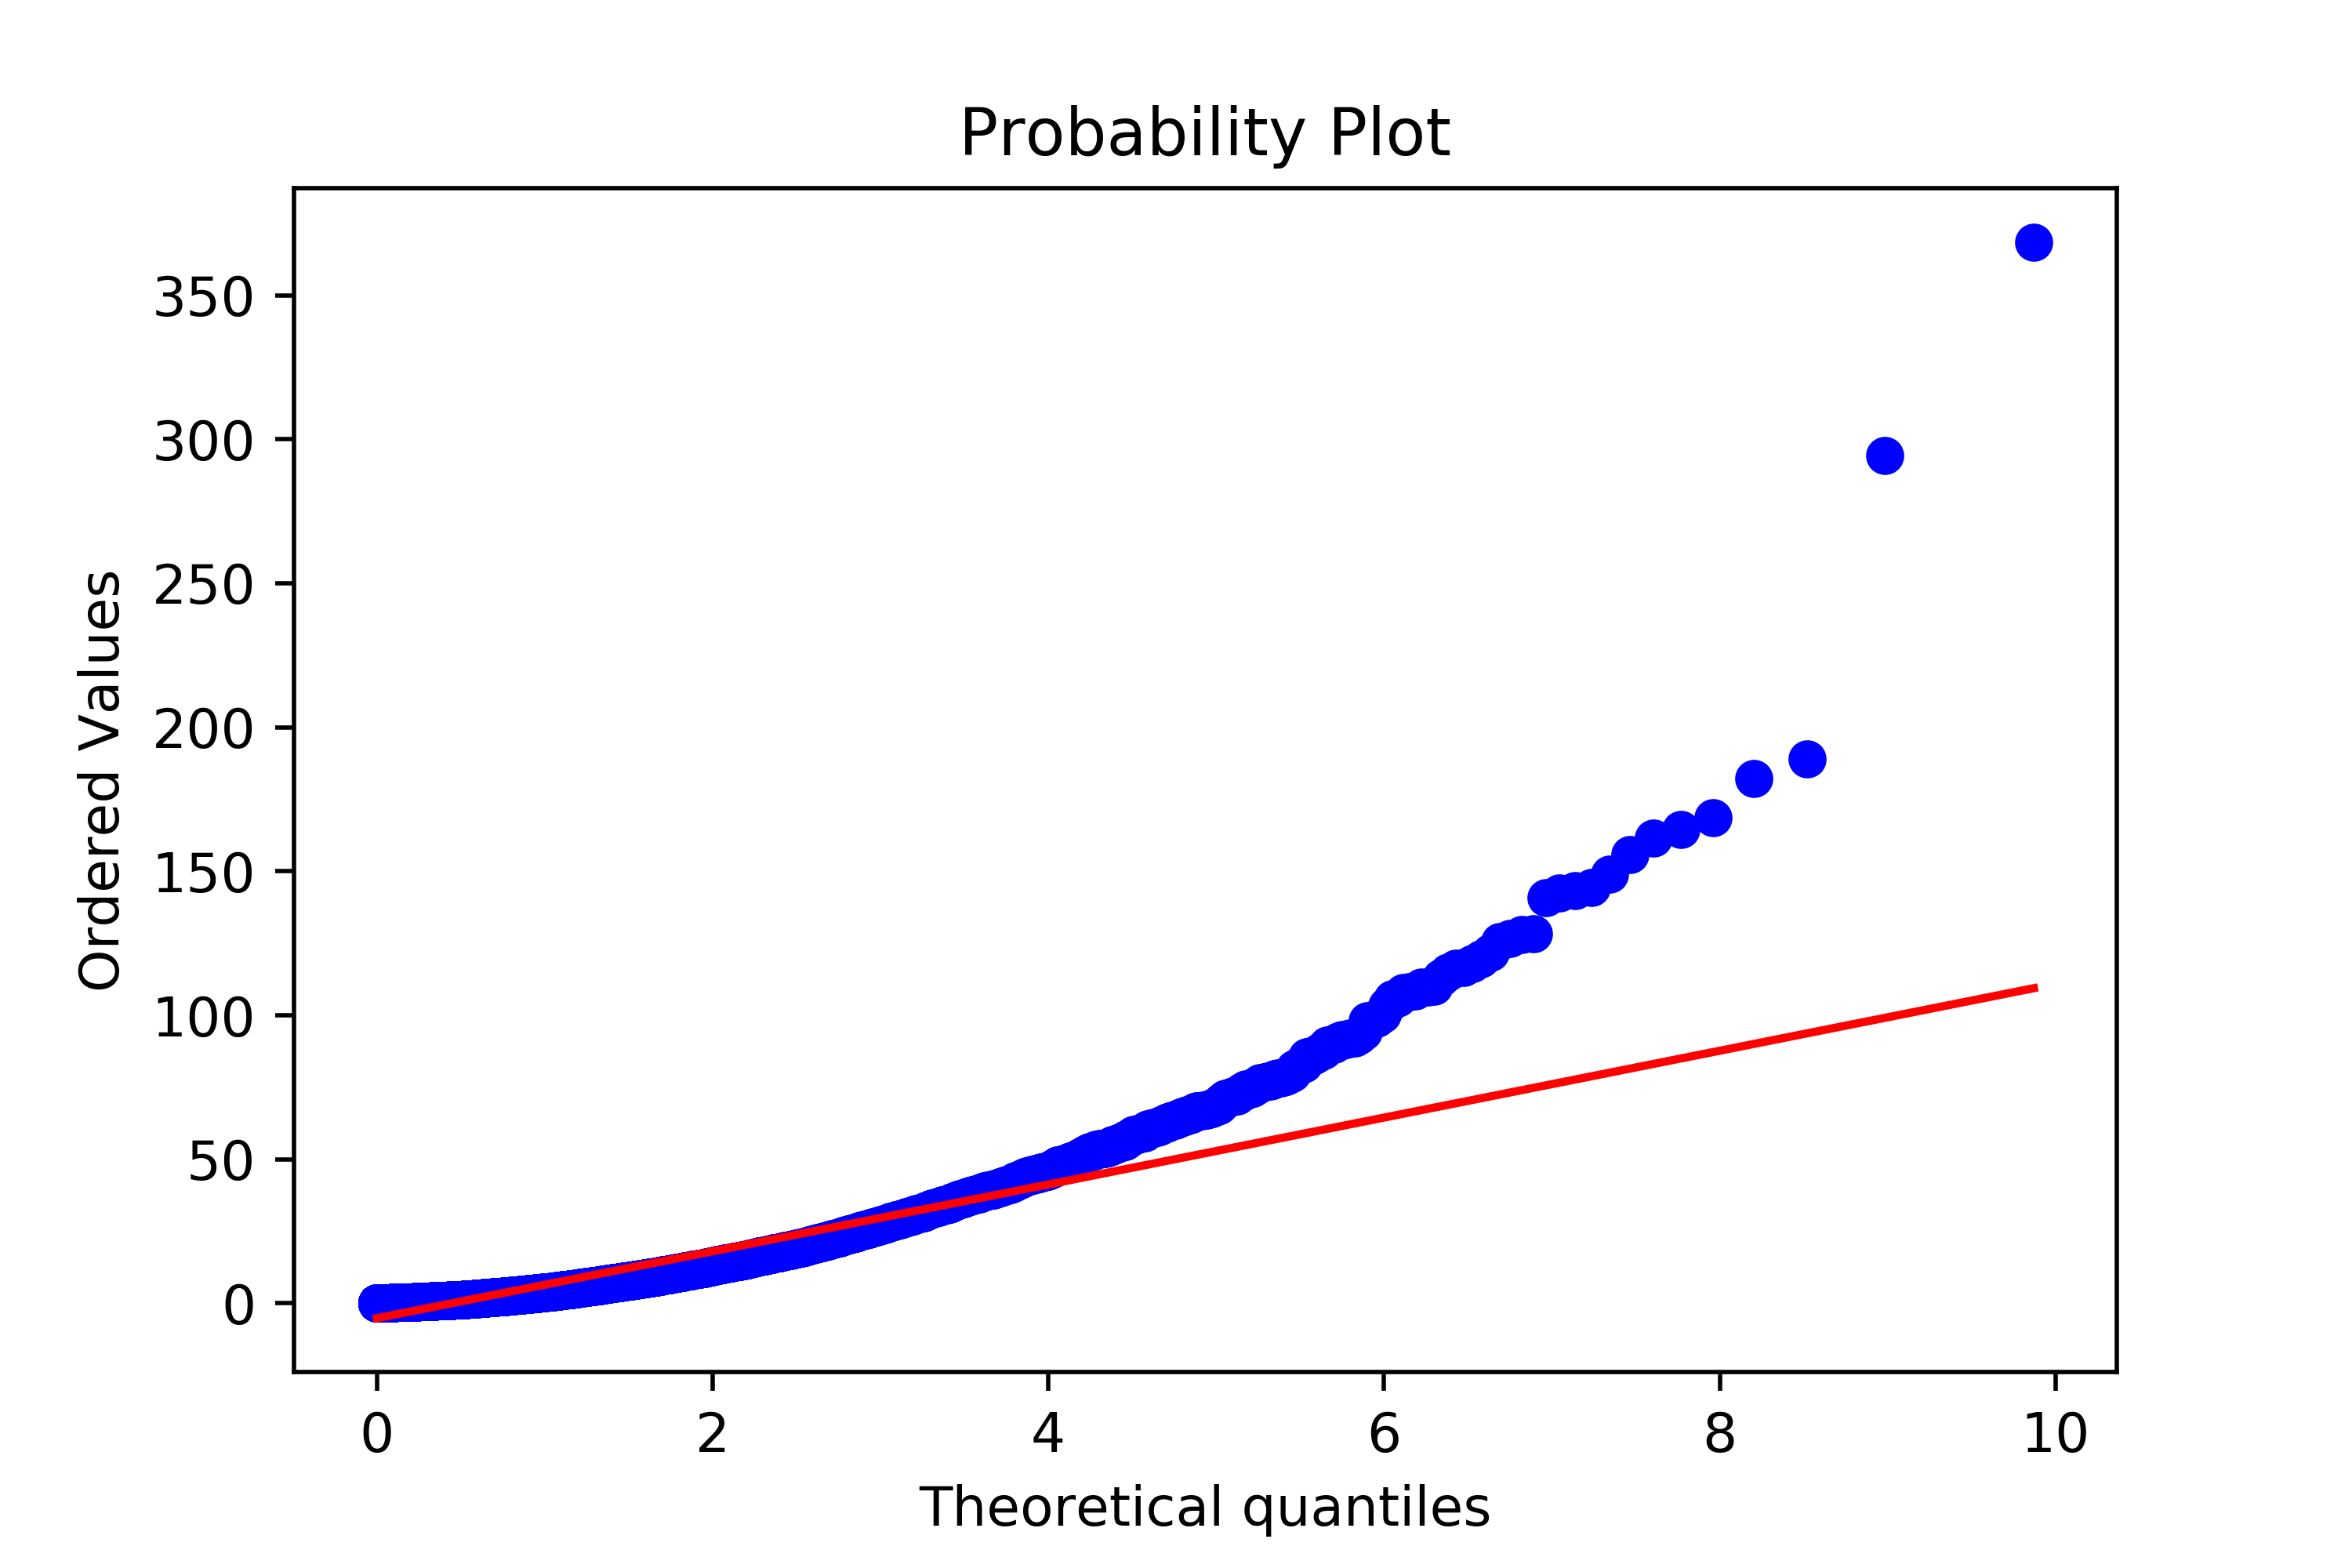
\includegraphics[width=60mm]{Figures/QQ_pos_k2.png}}
{}
&
\subf{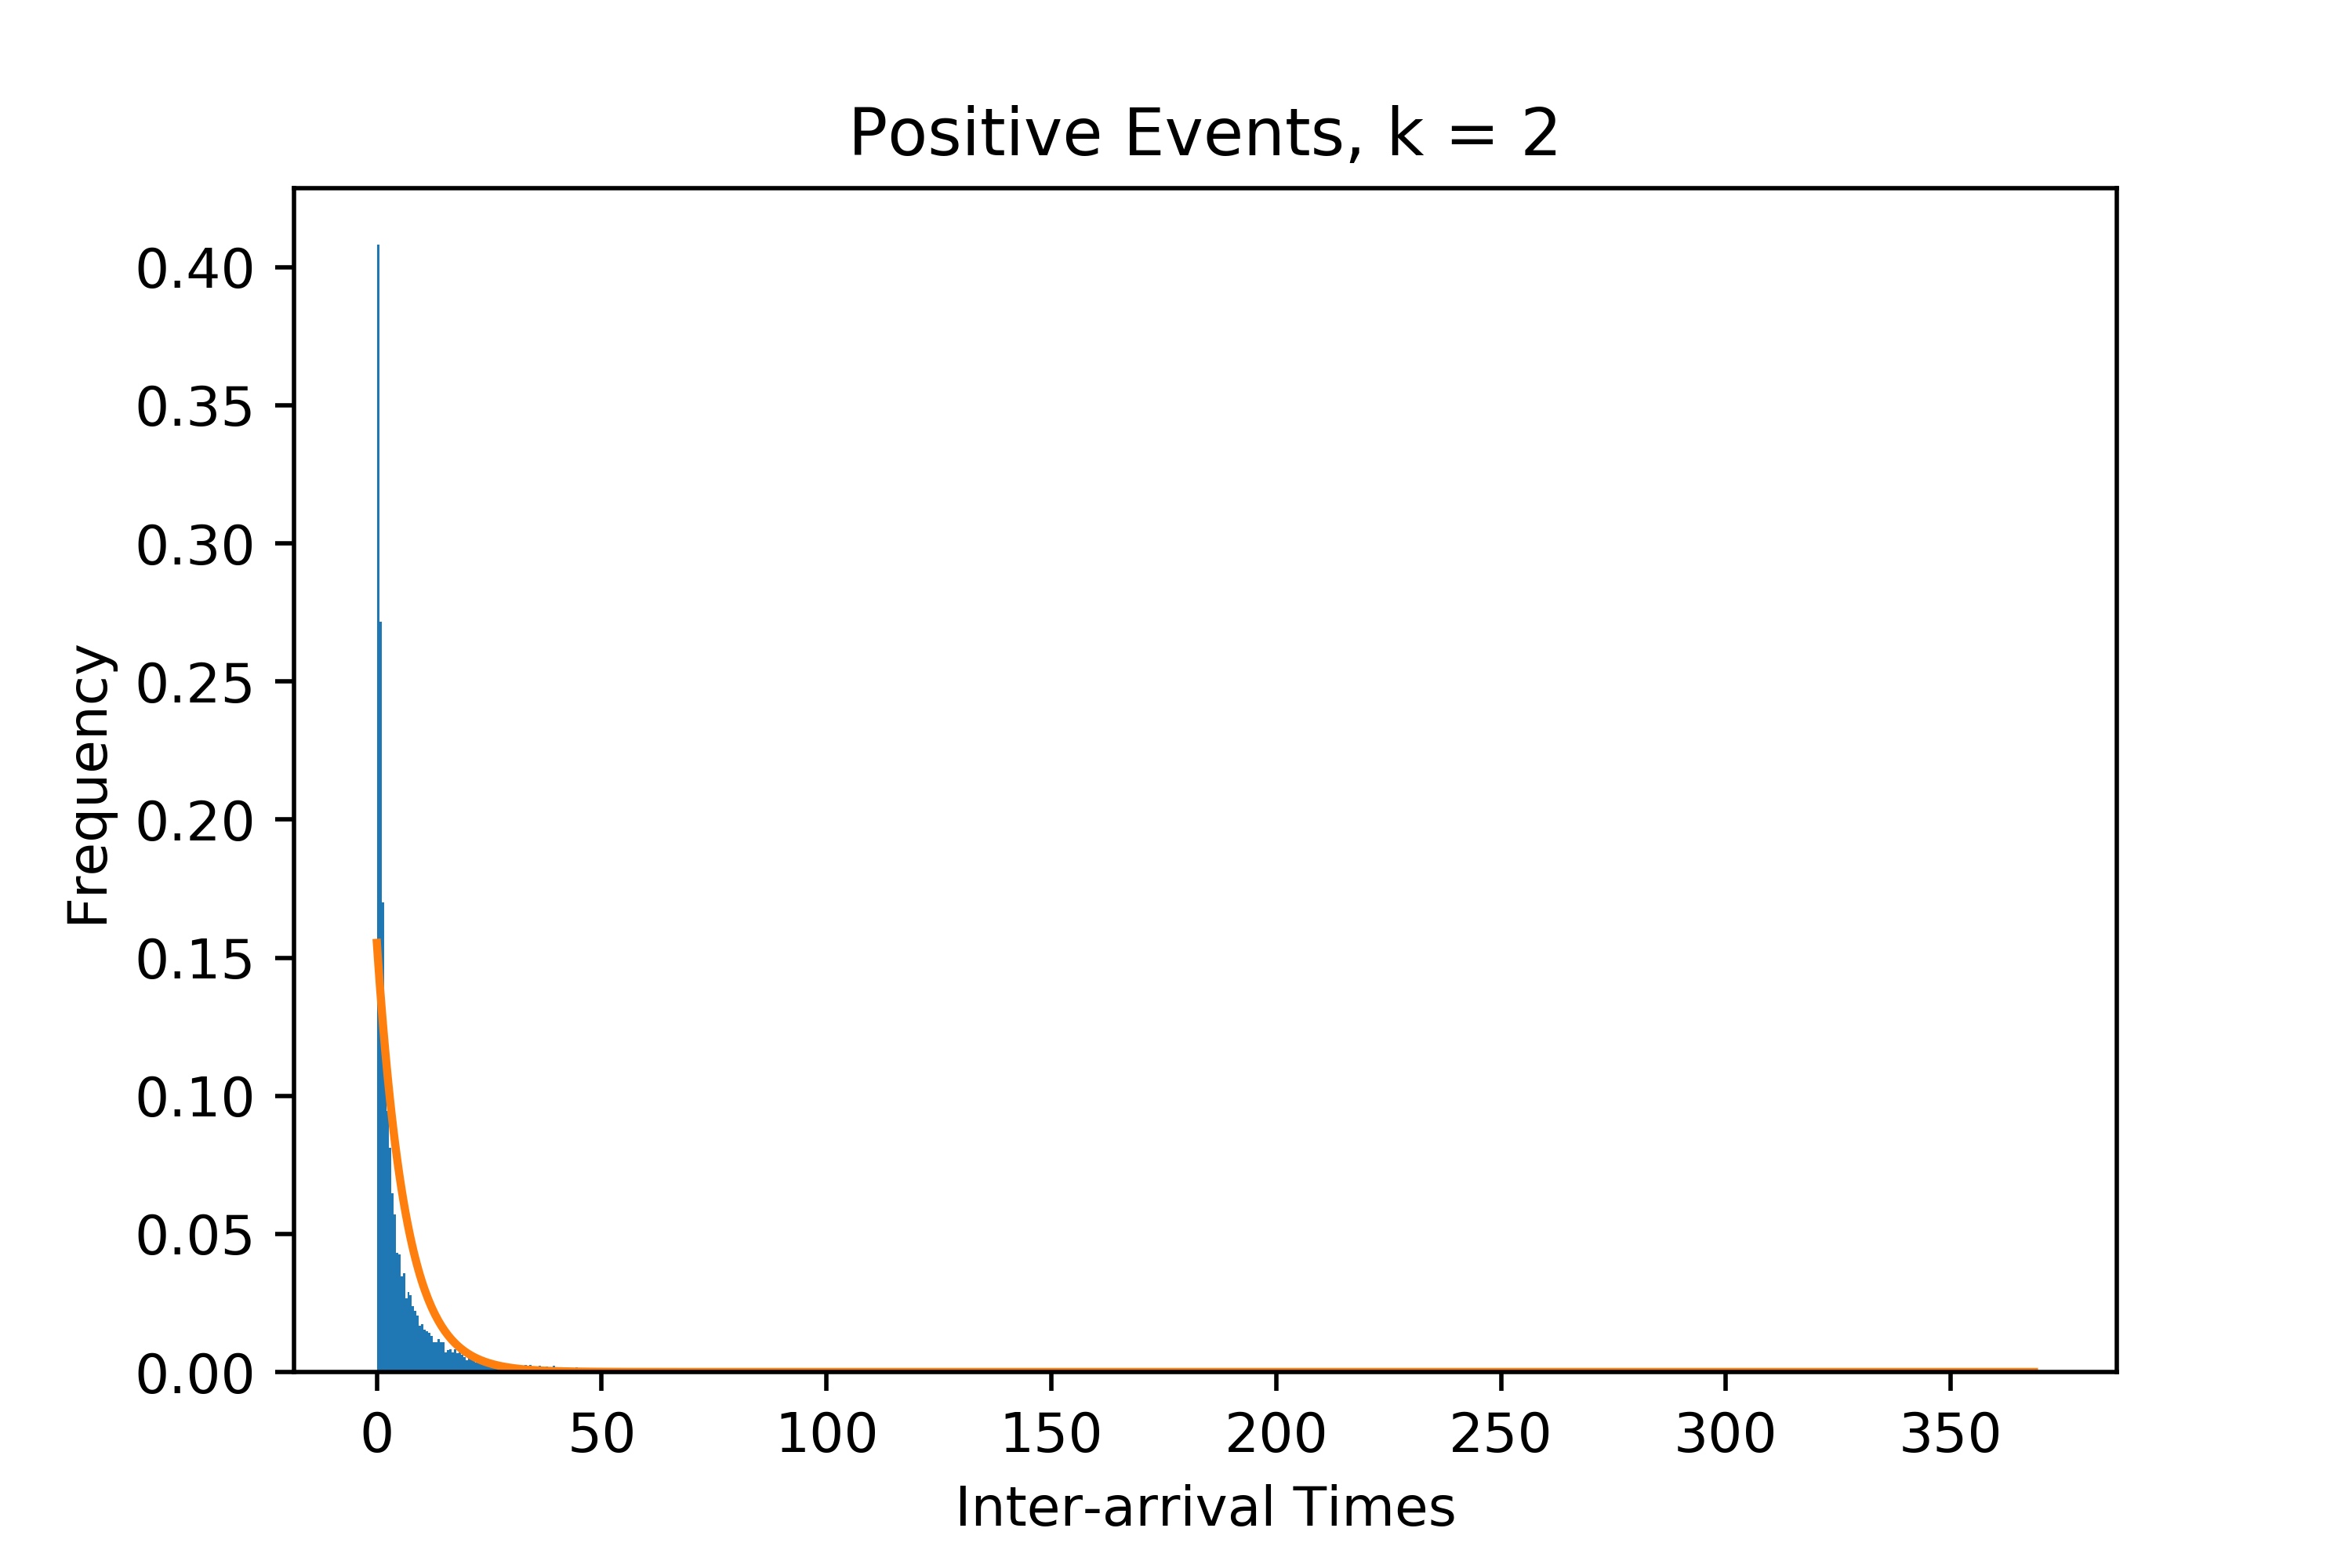
\includegraphics[width=60mm]{Figures/hist_pos_k2.png}}
{}
\\
\hline
\end{tabular}
\label{fig:interarrivals_pos}
\end{figure}

\begin{figure}
\centering
\caption{Inter-Arrival Times for Negative Events Compared to Exponential Distribution using Data from December 28-30, 2018}
\begin{tabular}{cc}
\hline
\subf{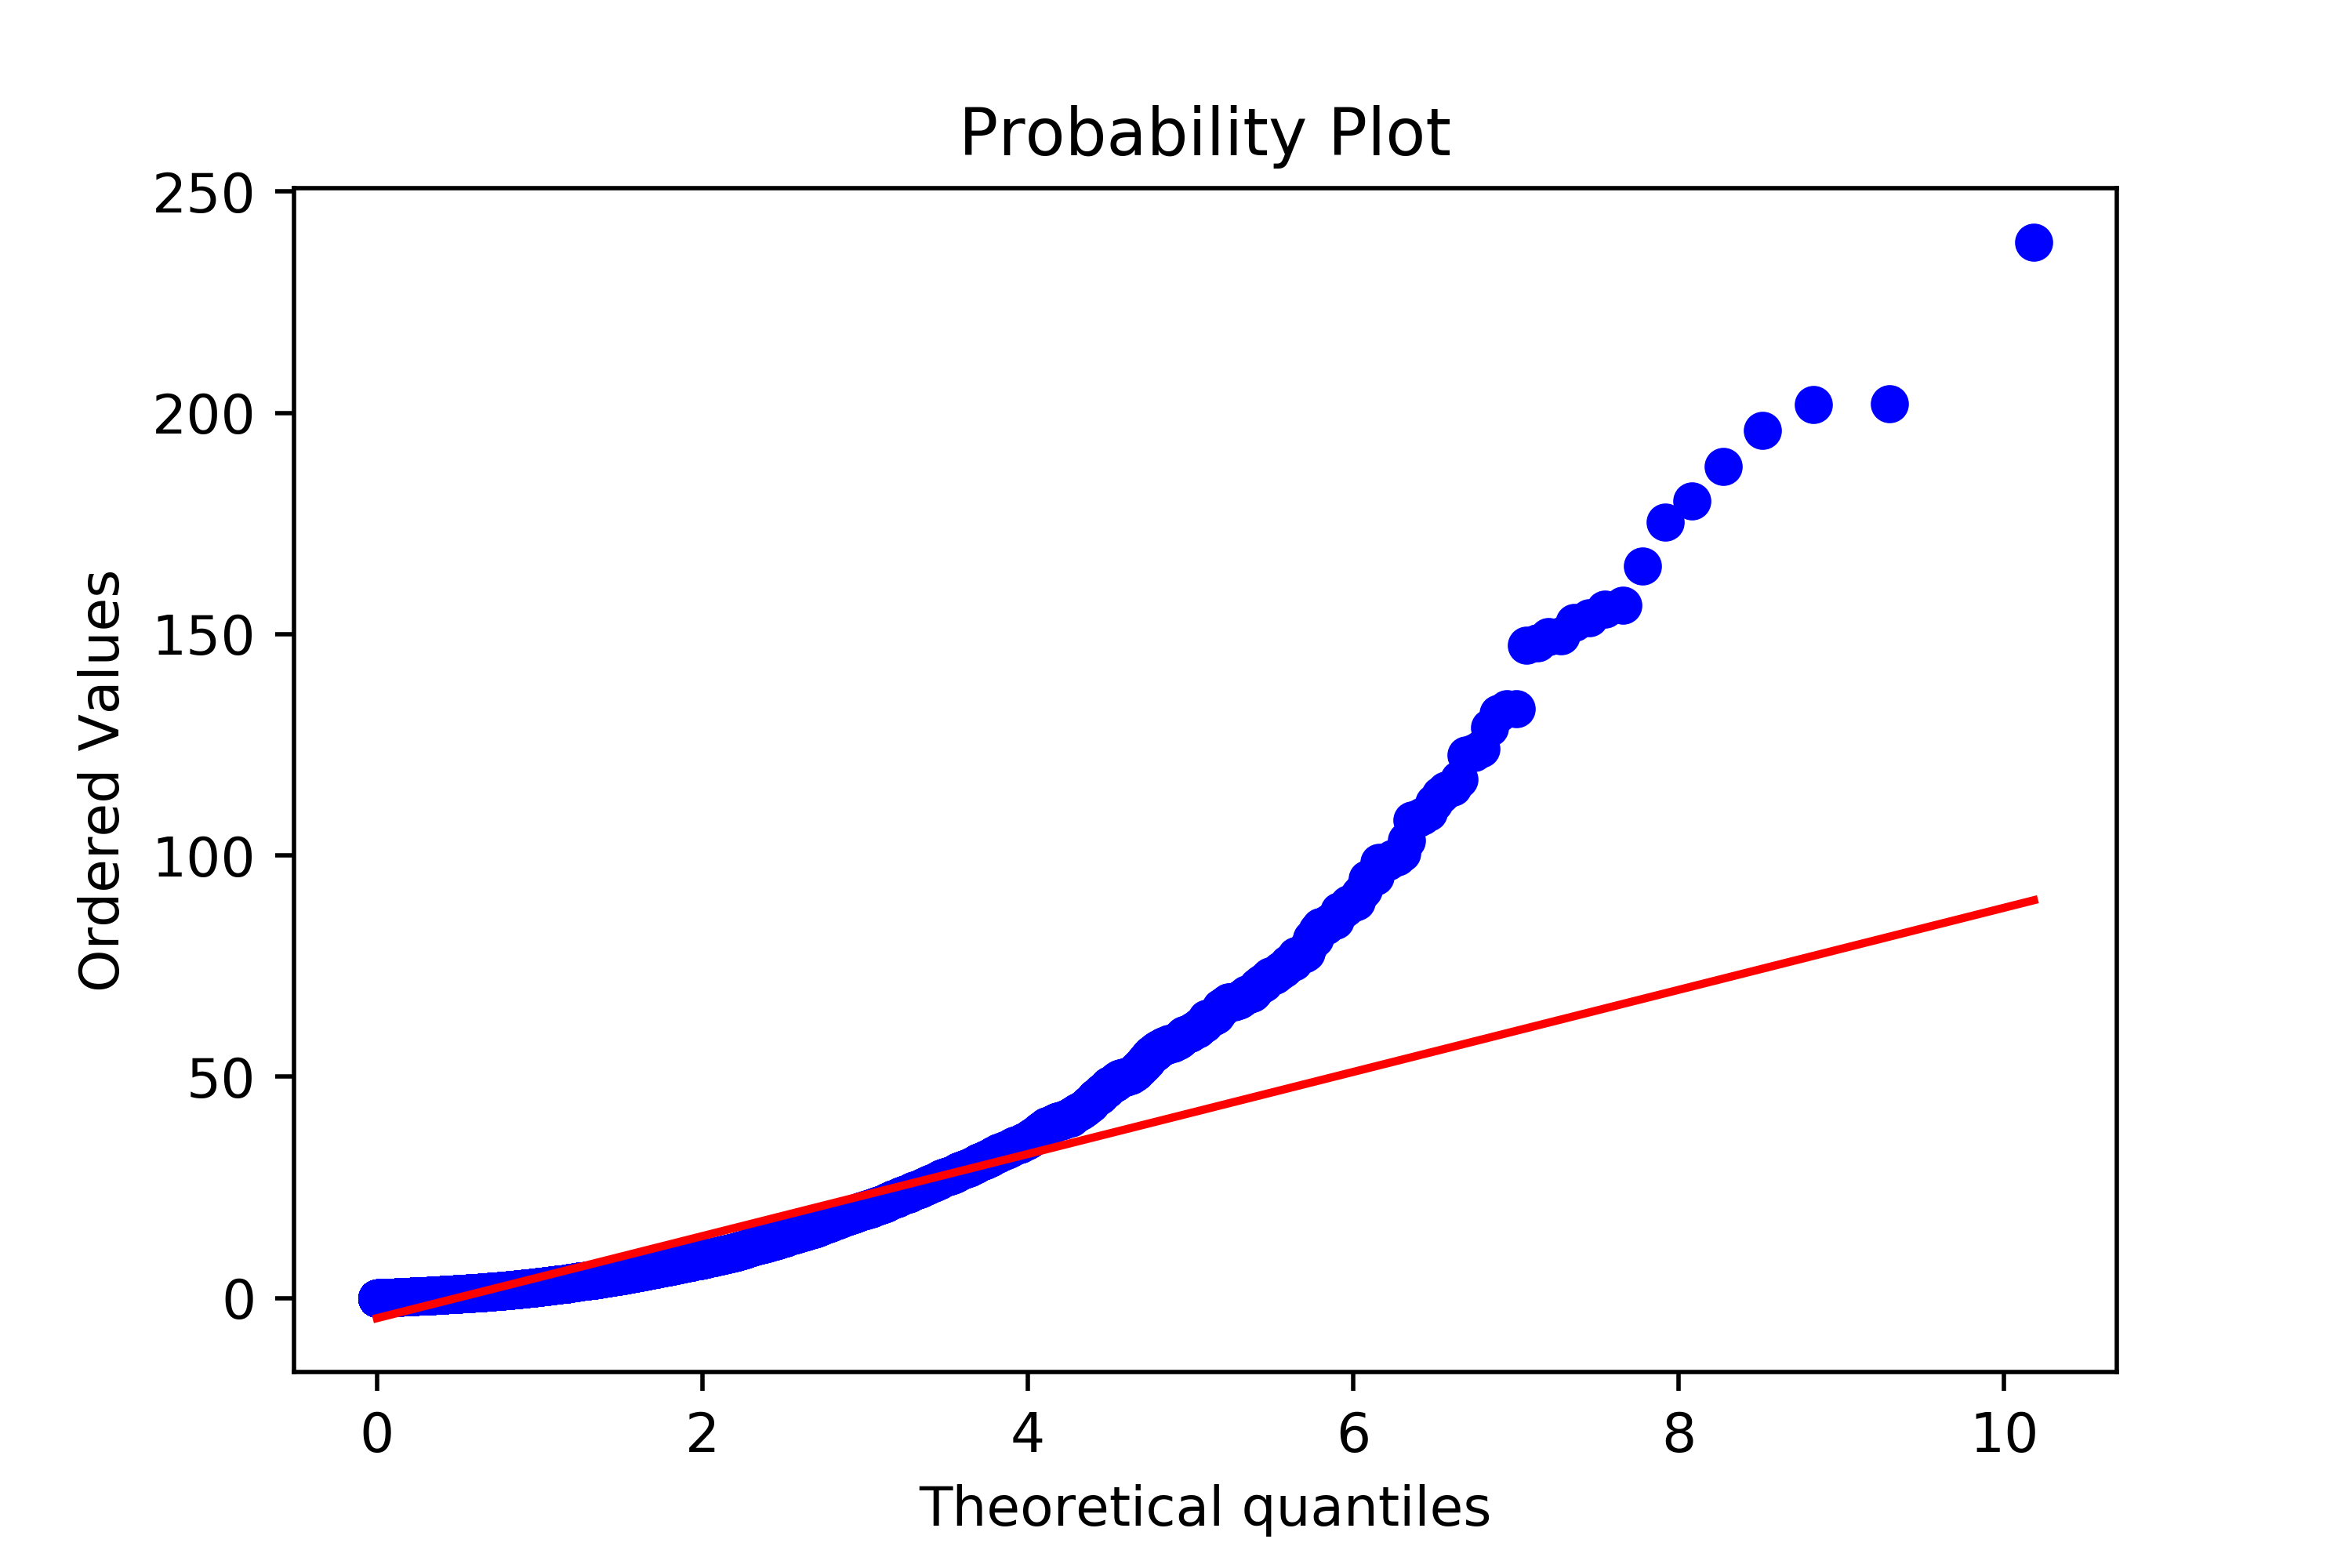
\includegraphics[width=60mm]{Figures/QQ_neg_k-2.png}}
{}
&
\subf{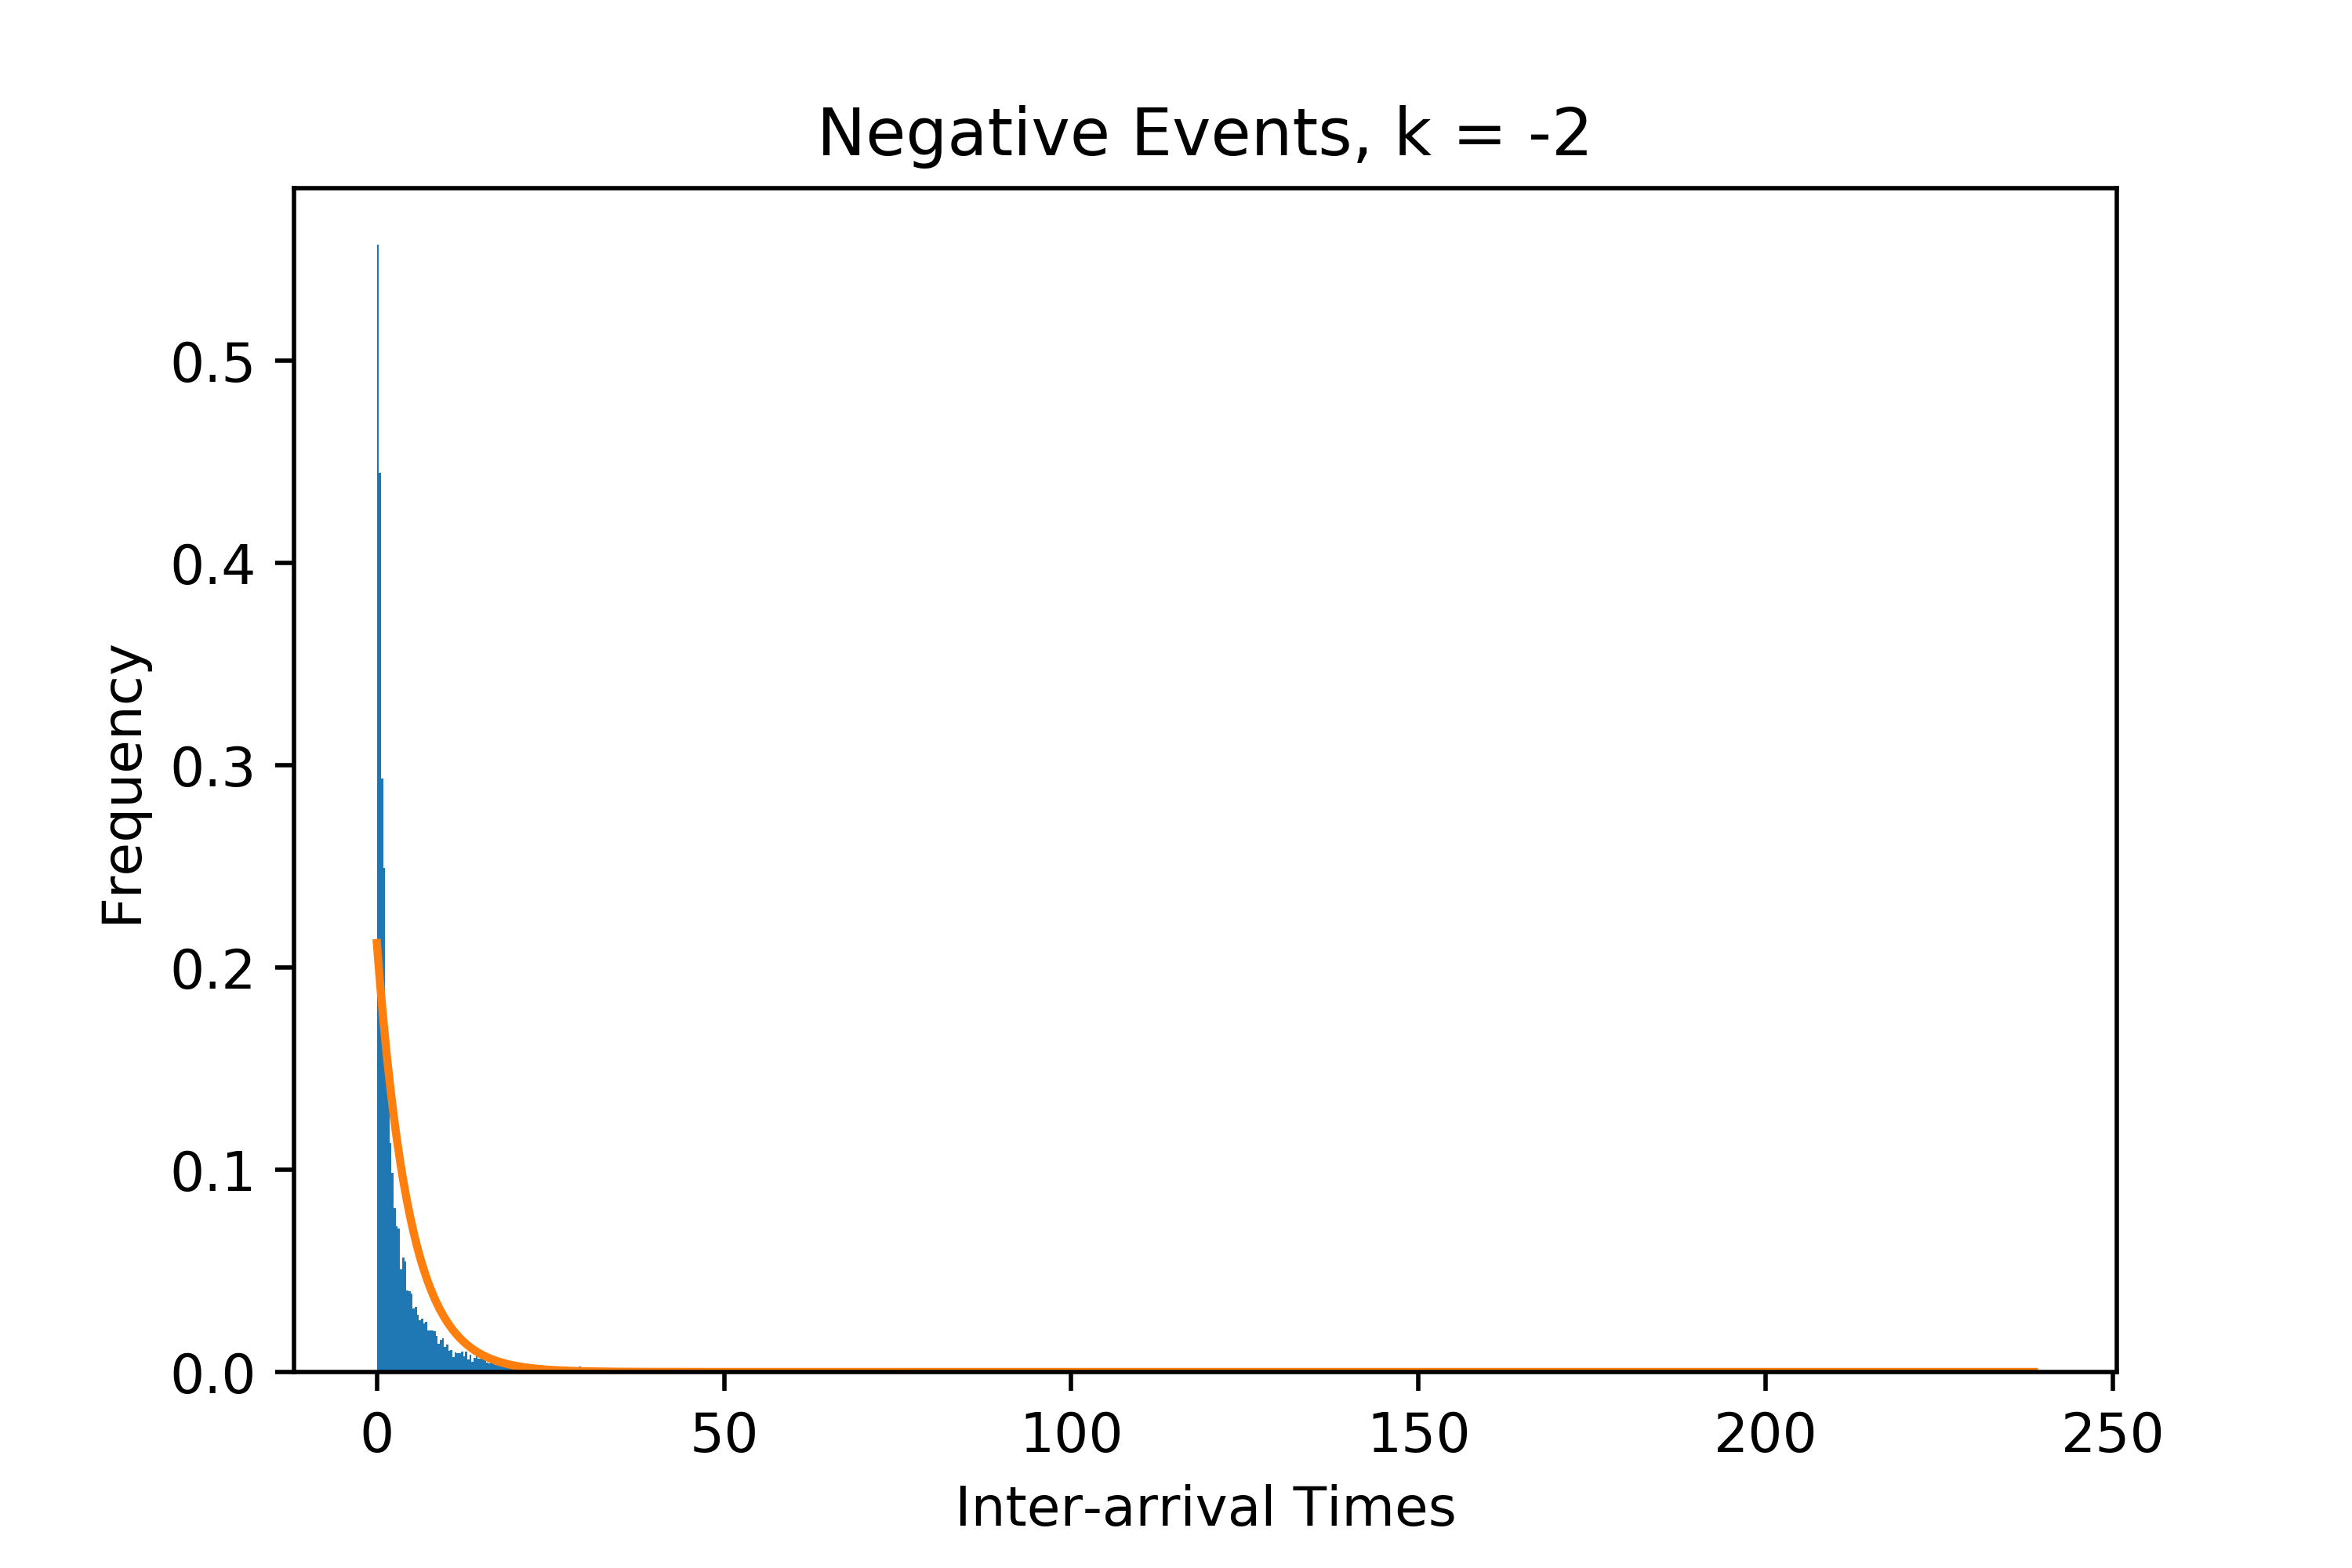
\includegraphics[width=60mm]{Figures/hist_neg_k-2.png}}
{}
\\
\subf{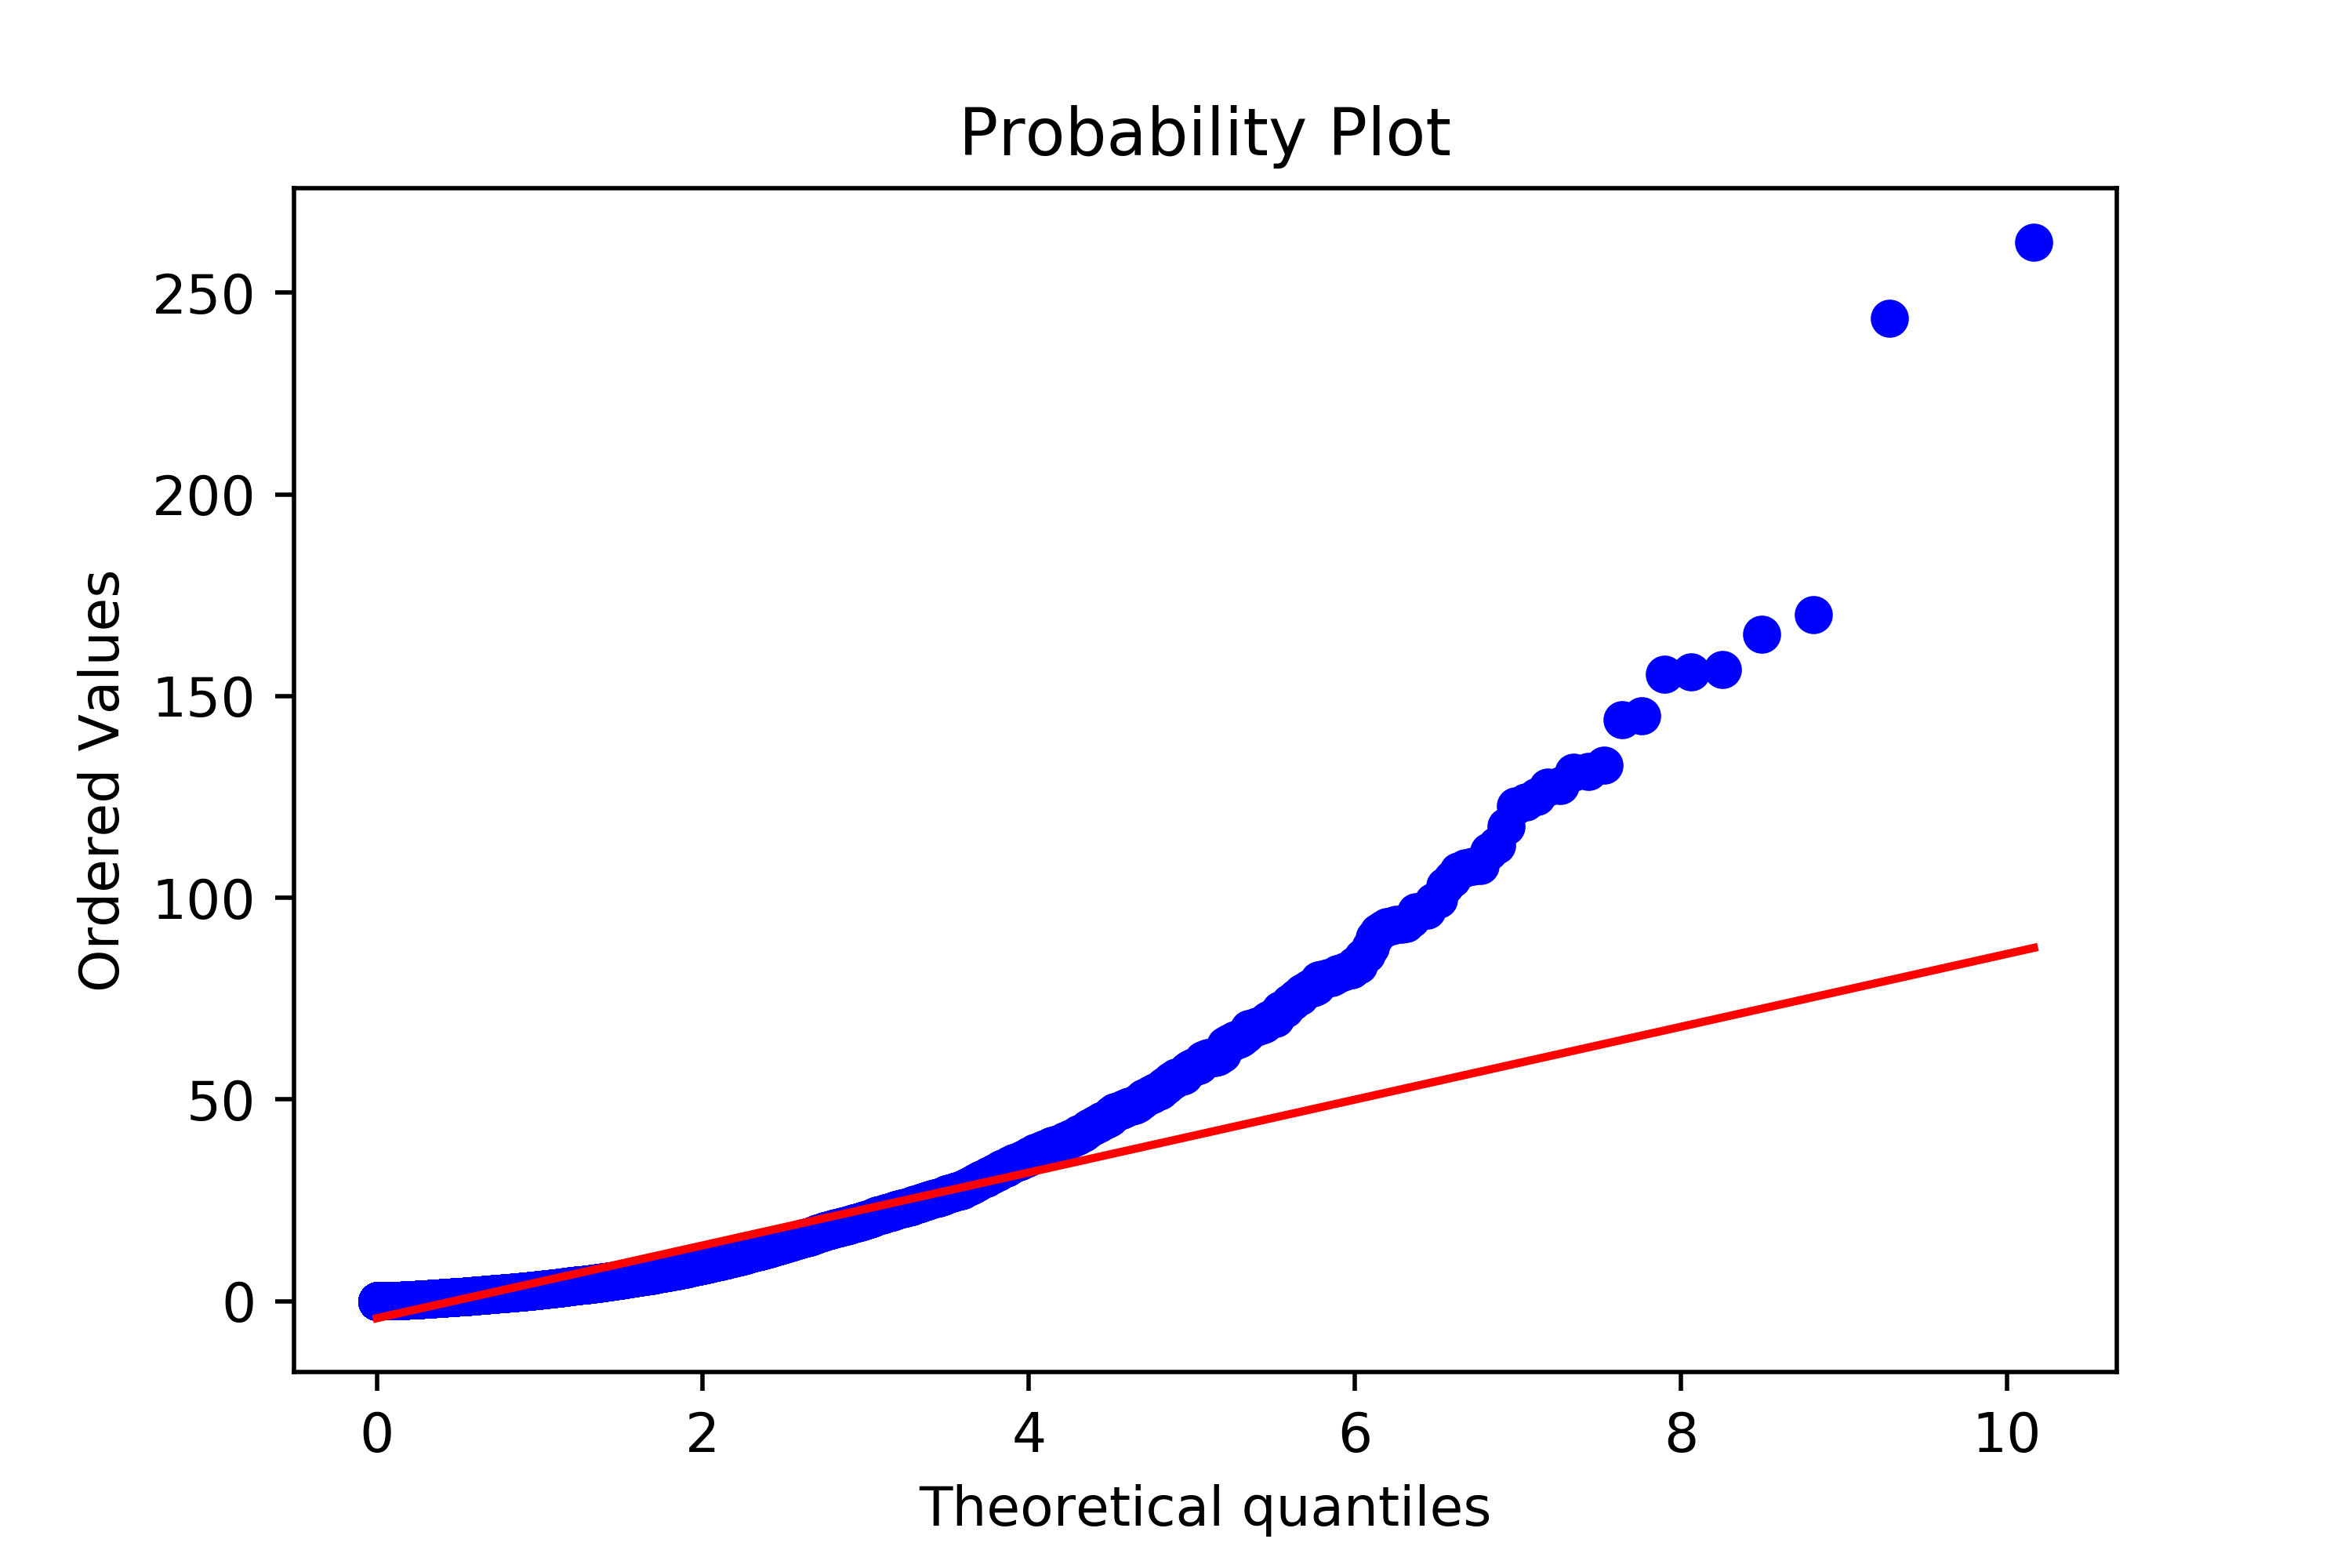
\includegraphics[width=60mm]{Figures/QQ_neg_k-1.png}}
{}
&
\subf{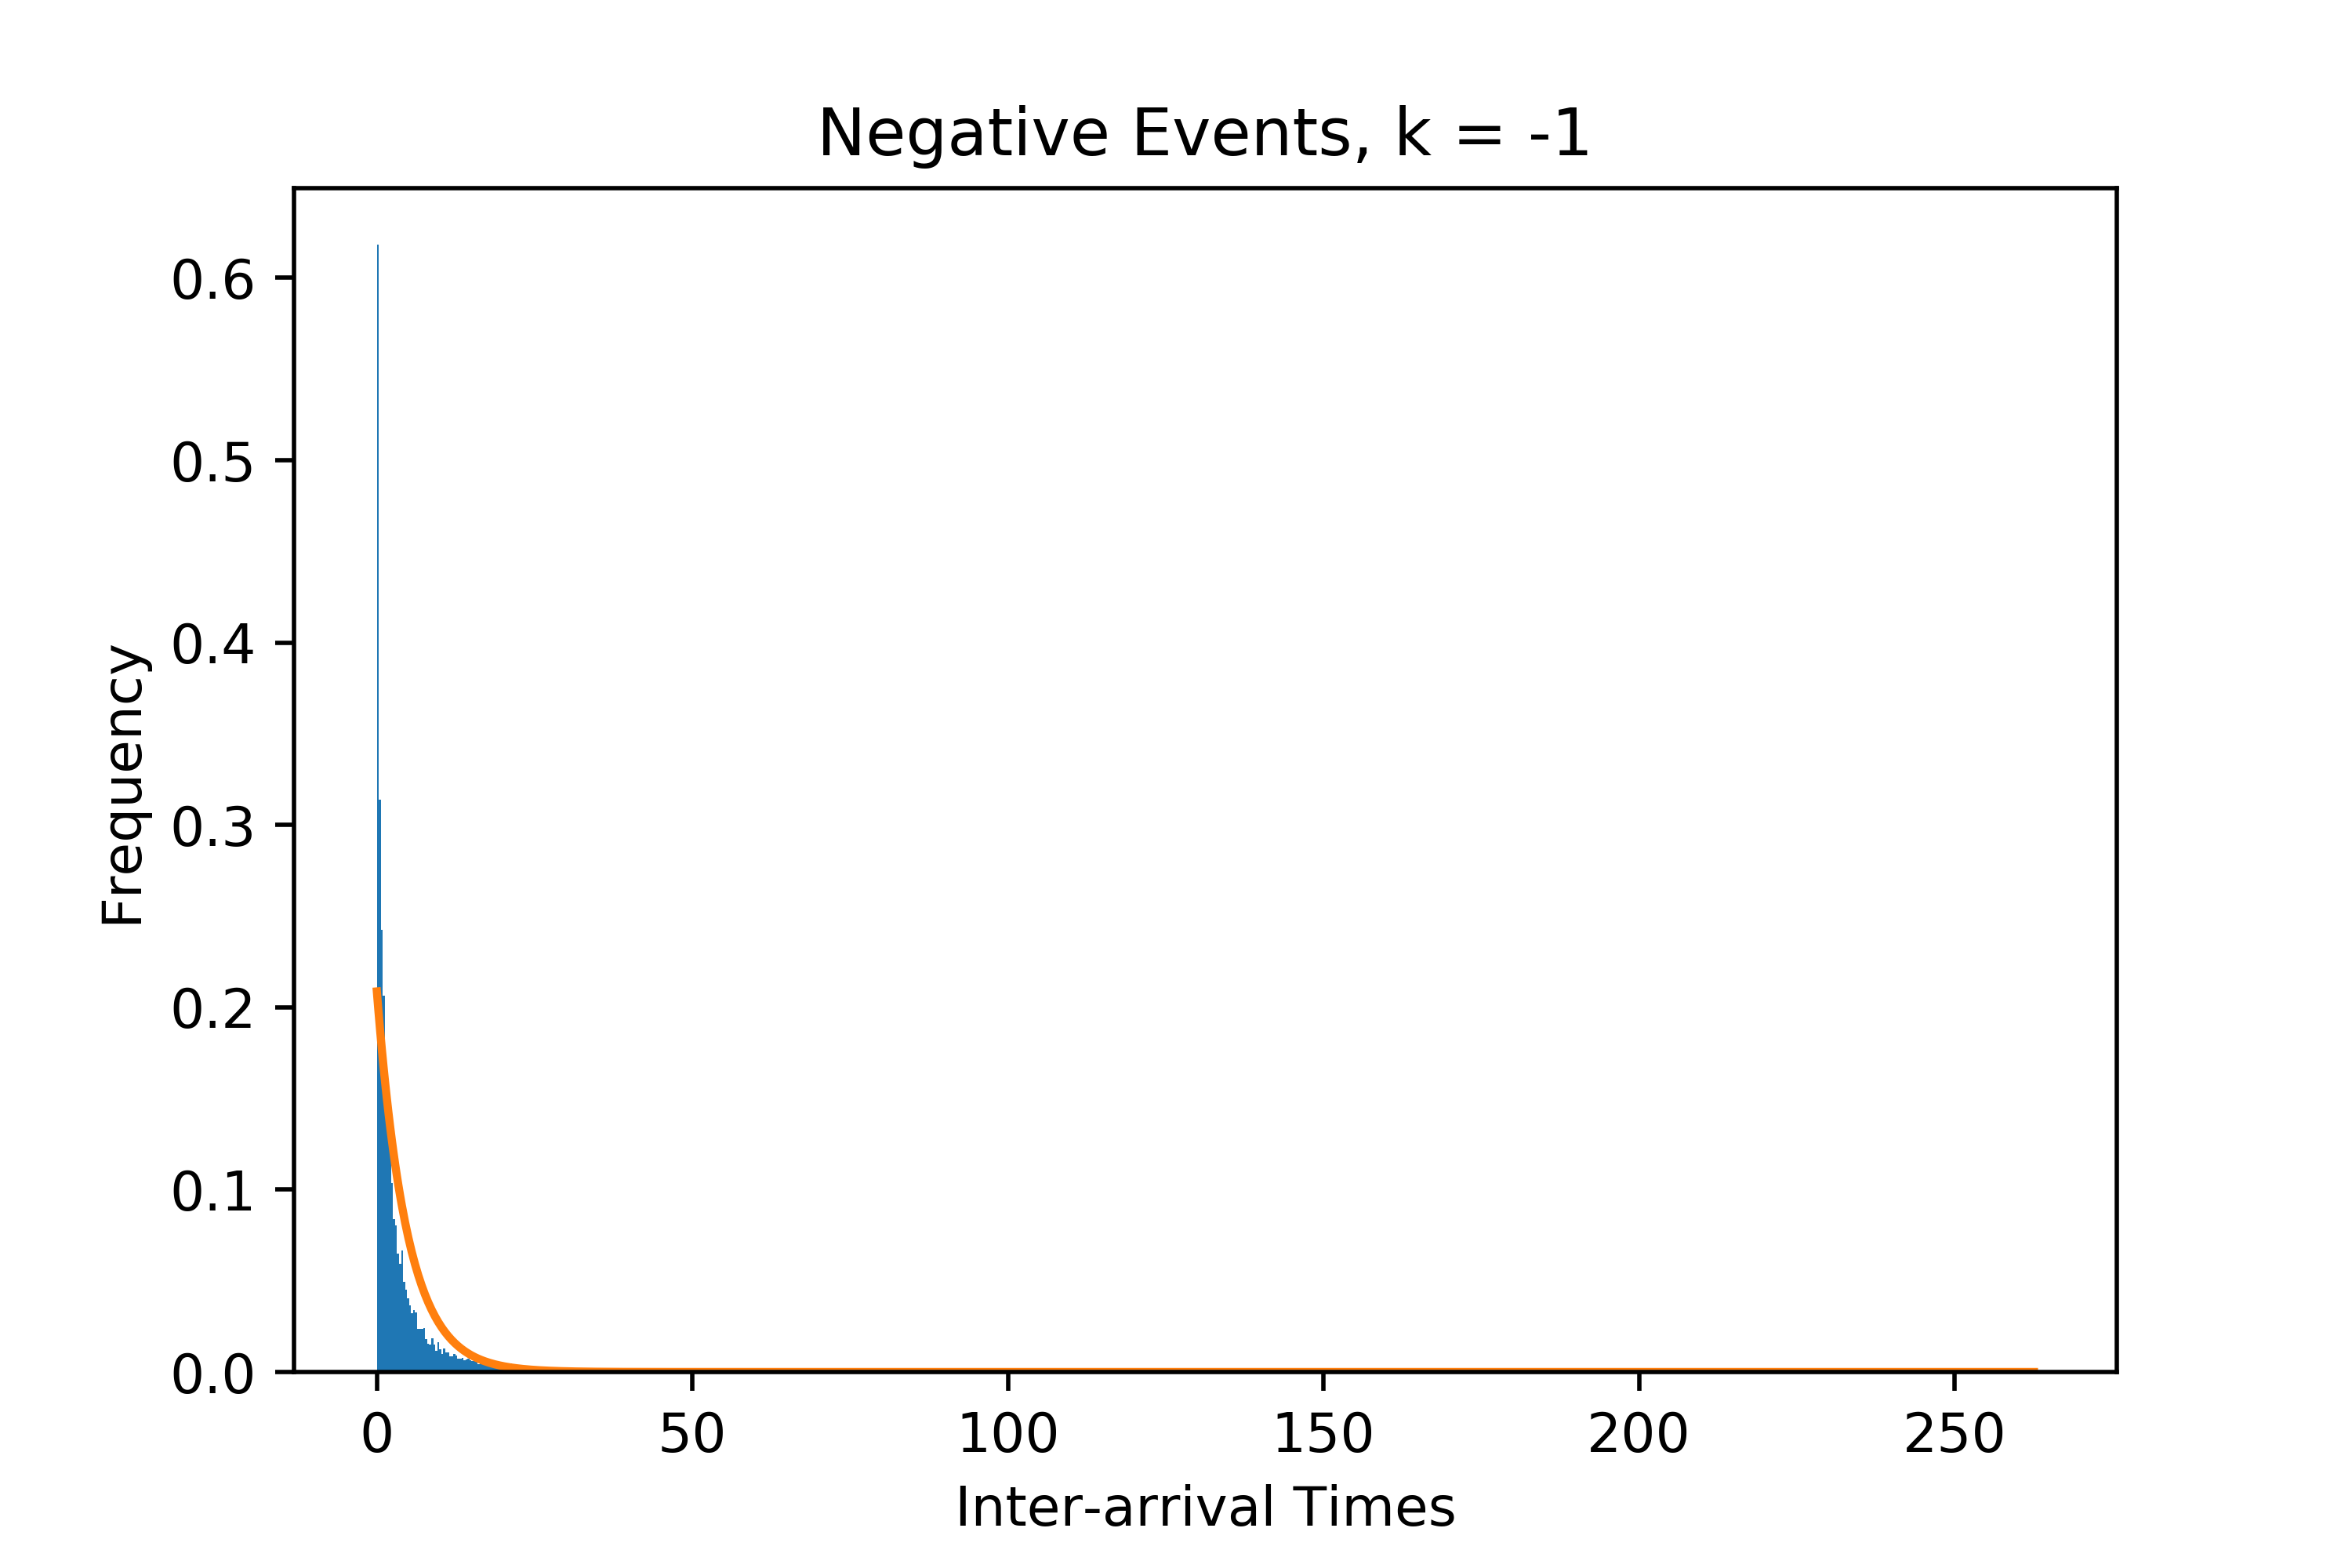
\includegraphics[width=60mm]{Figures/hist_neg_k-1.png}}
{}
\\
\subf{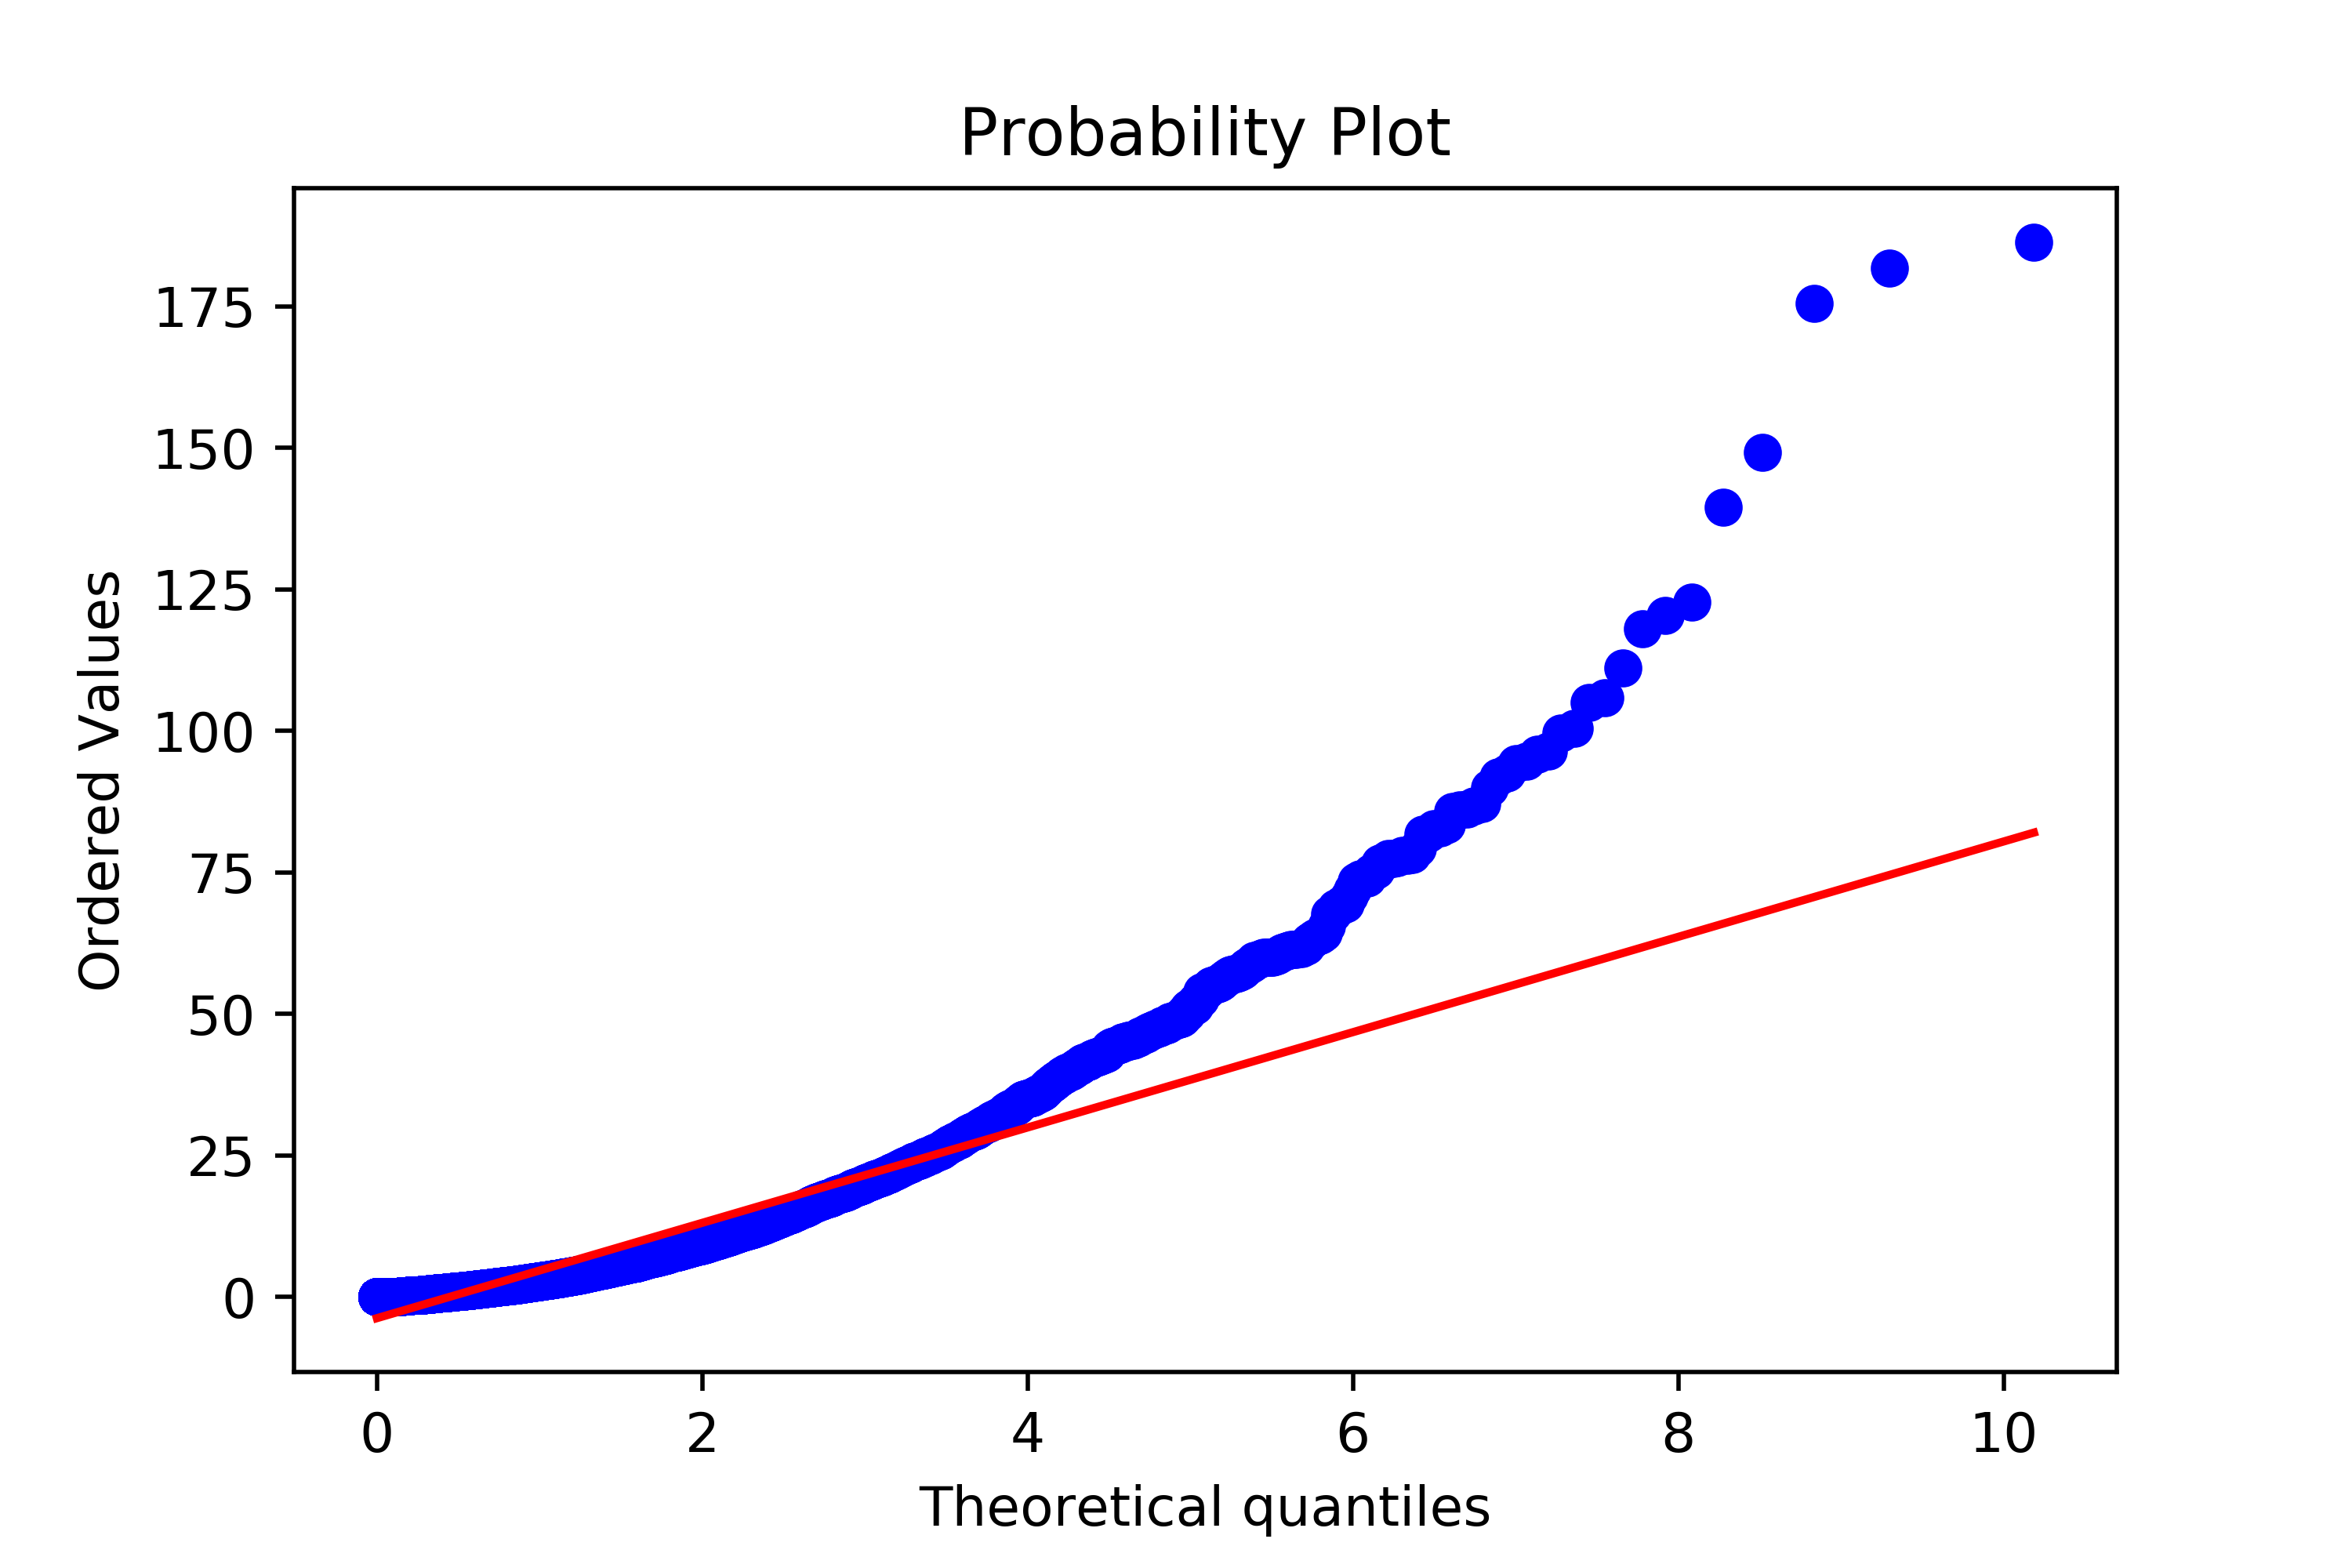
\includegraphics[width=60mm]{Figures/QQ_neg_k1.png}}
{}
&
\subf{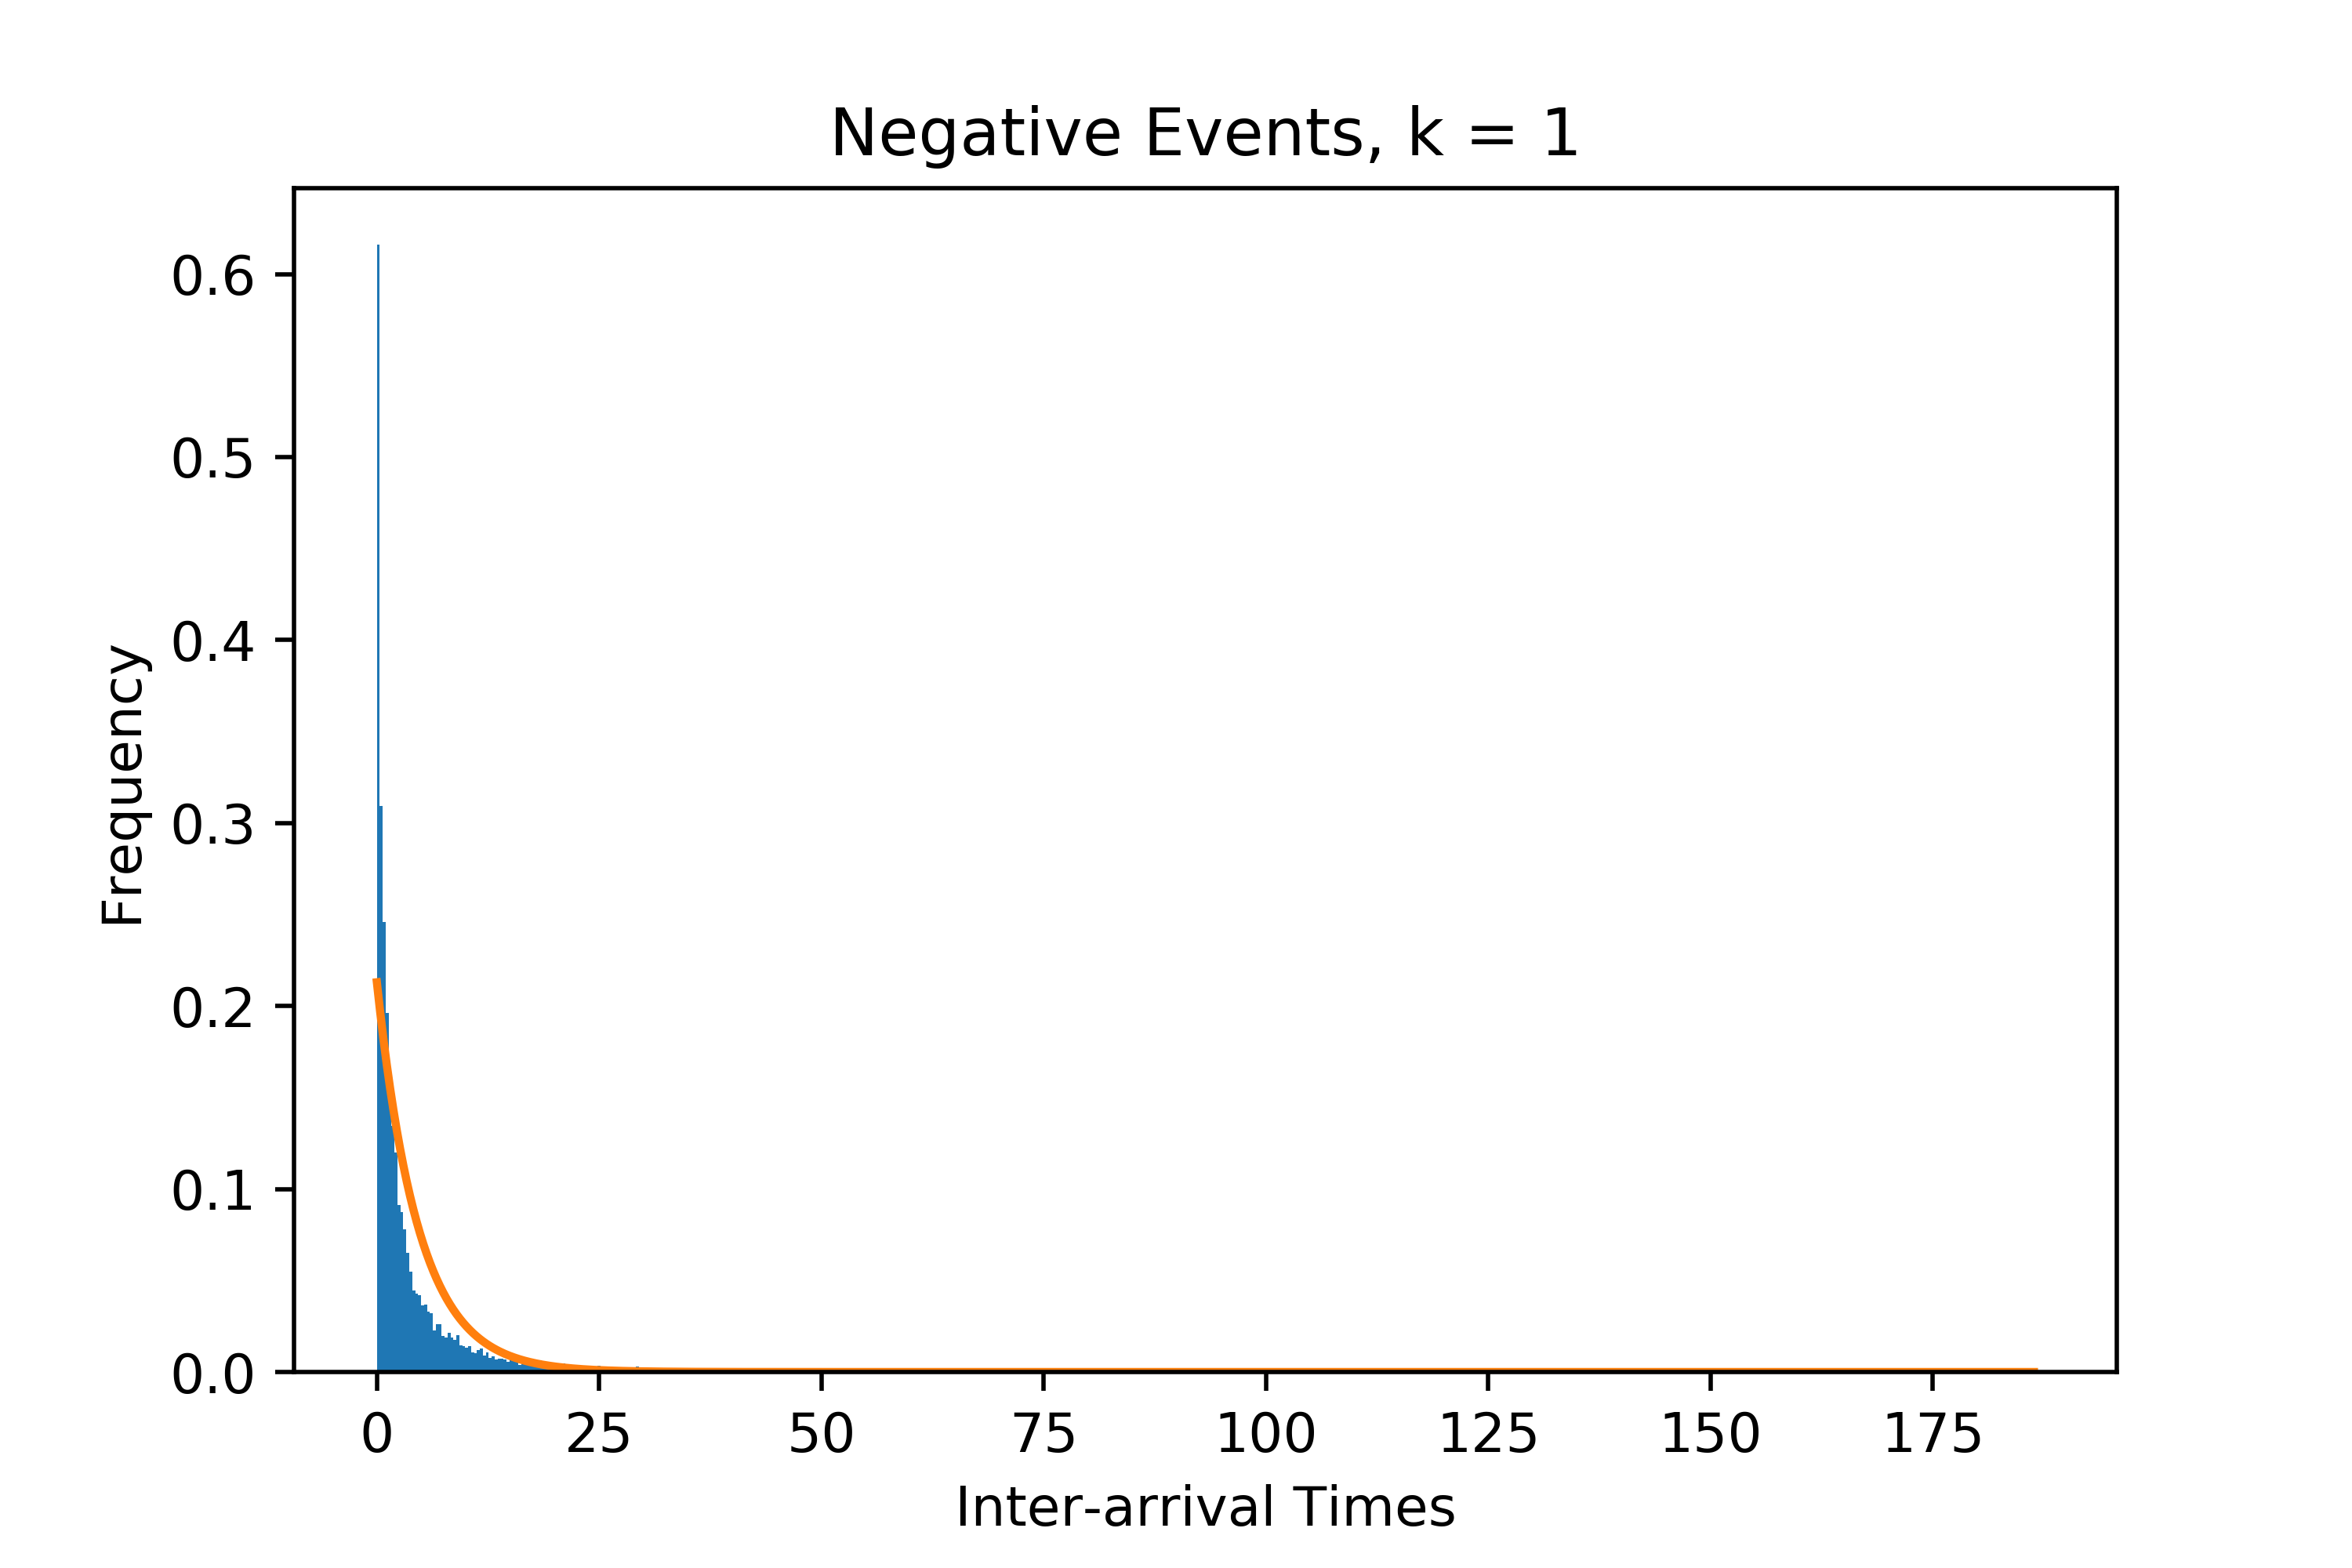
\includegraphics[width=60mm]{Figures/hist_neg_k1.png}}
{}
\\
\subf{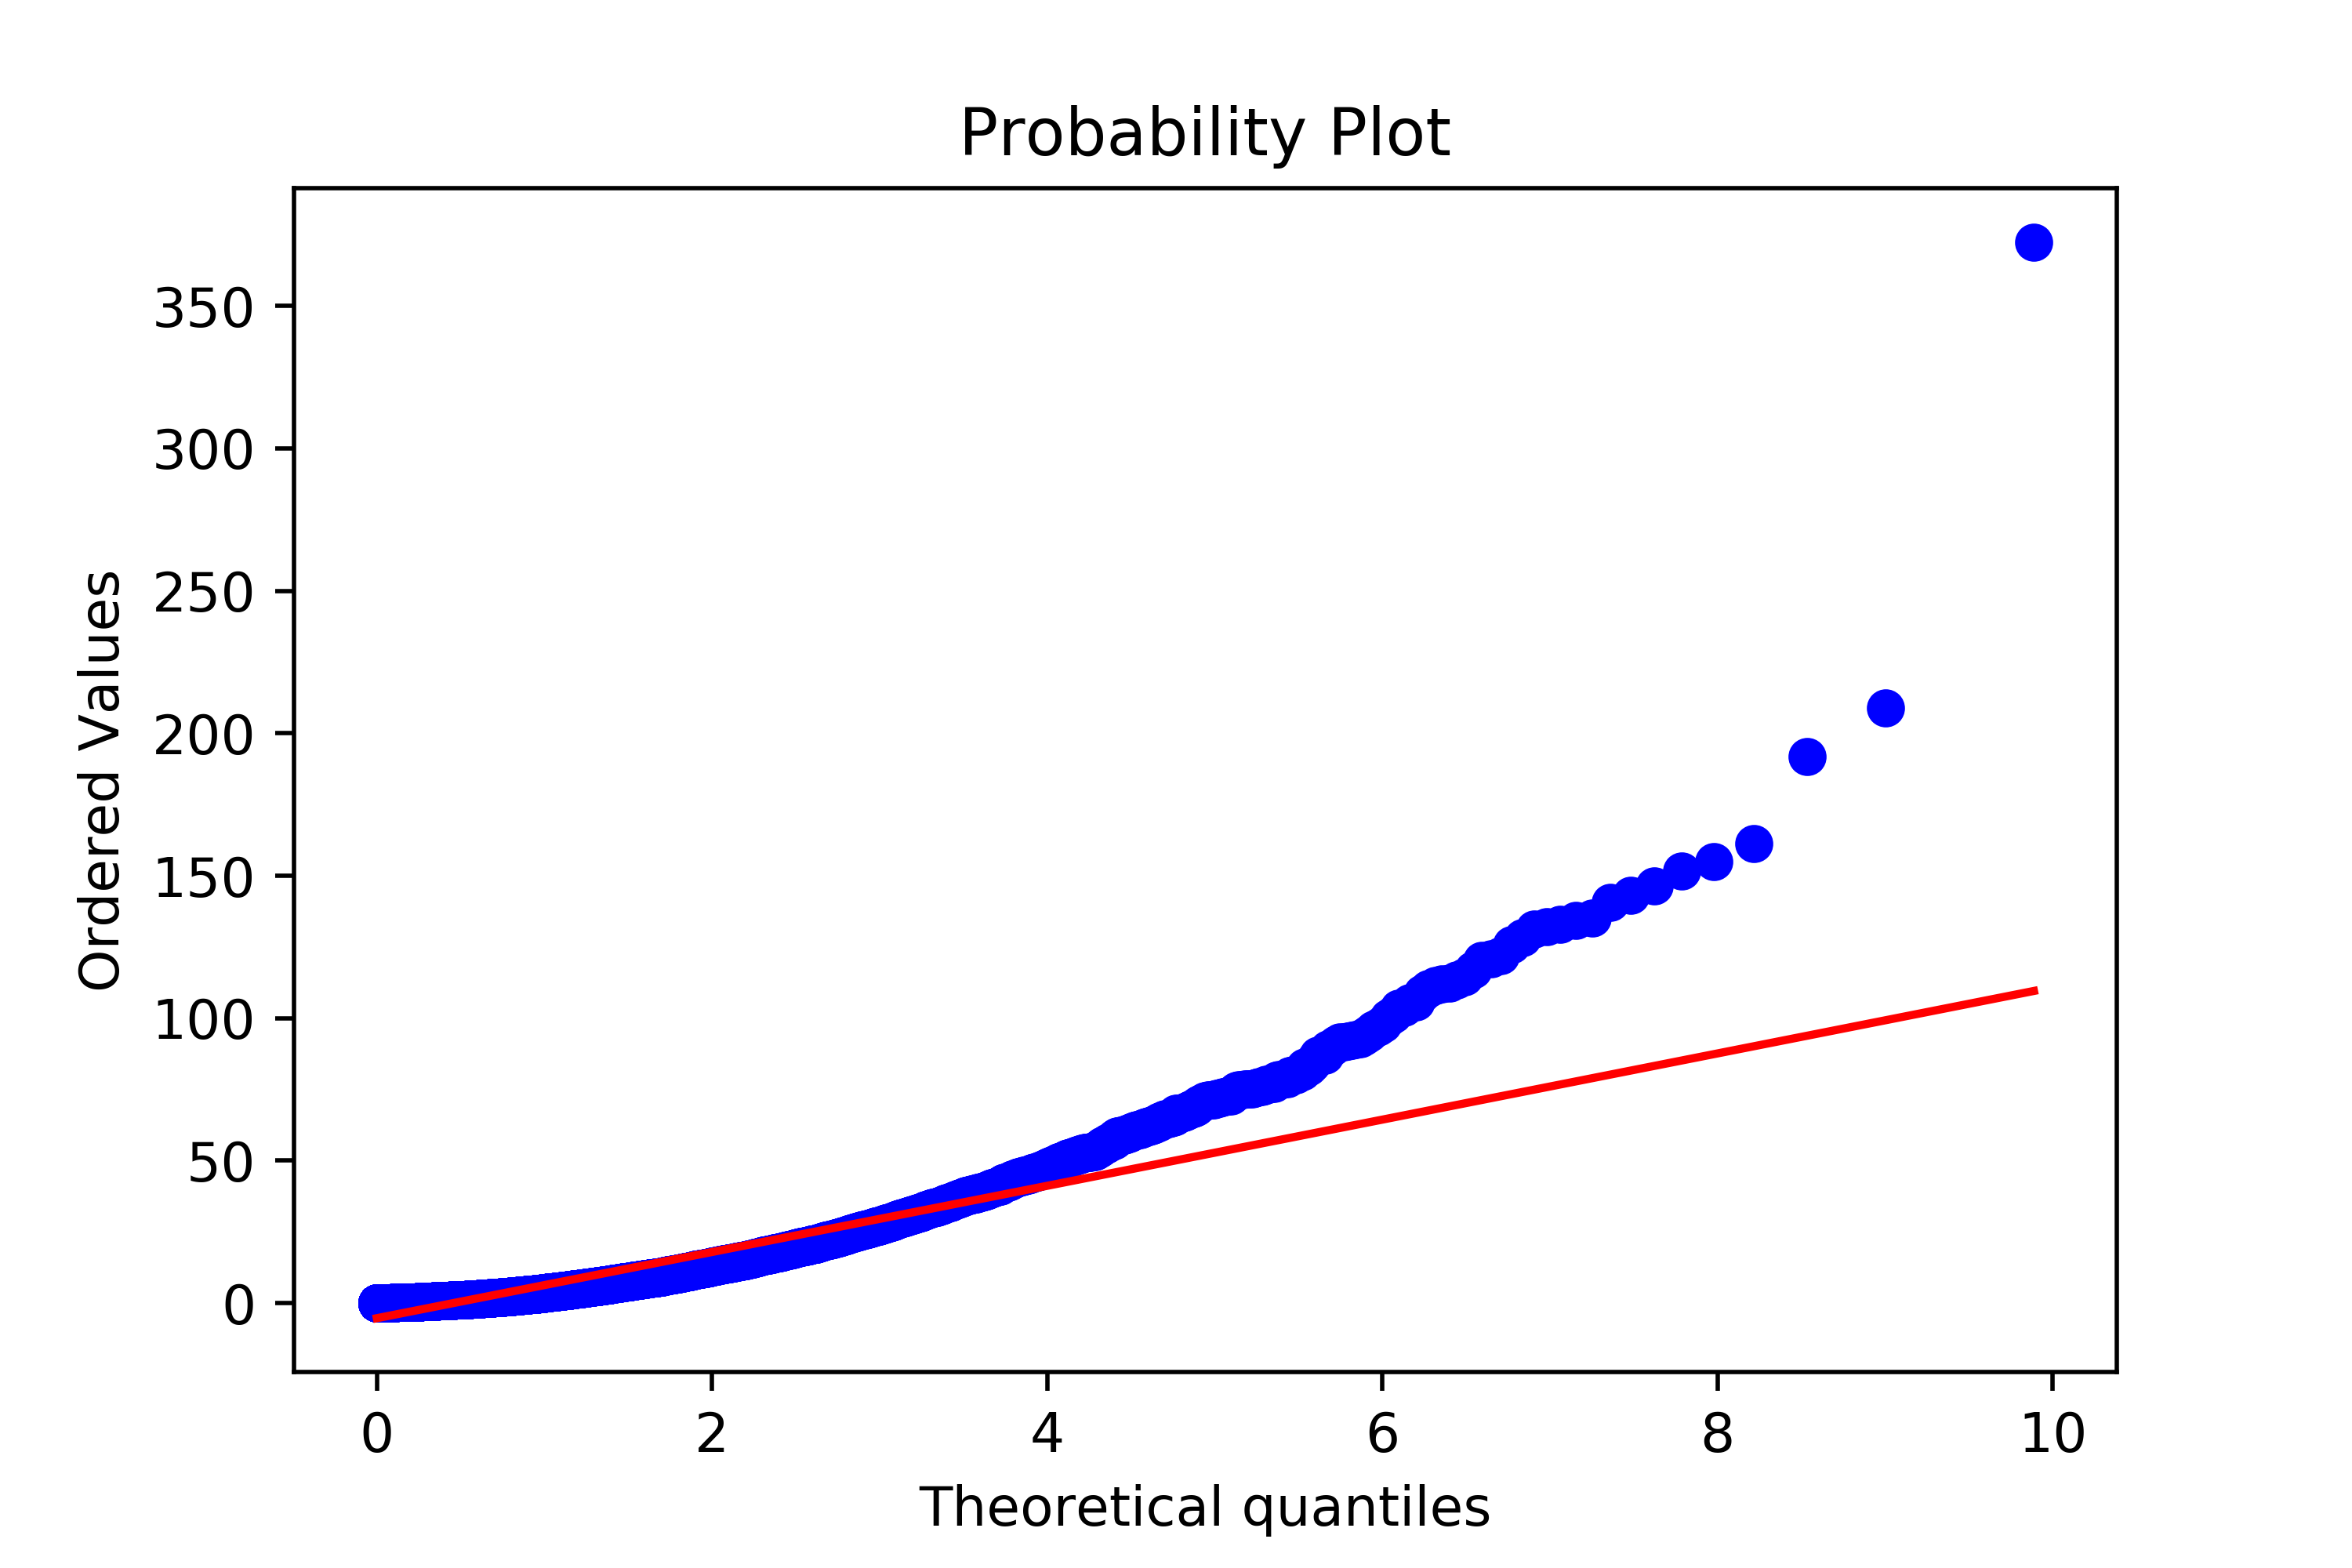
\includegraphics[width=60mm]{Figures/QQ_neg_k2.png}}
{}
&
\subf{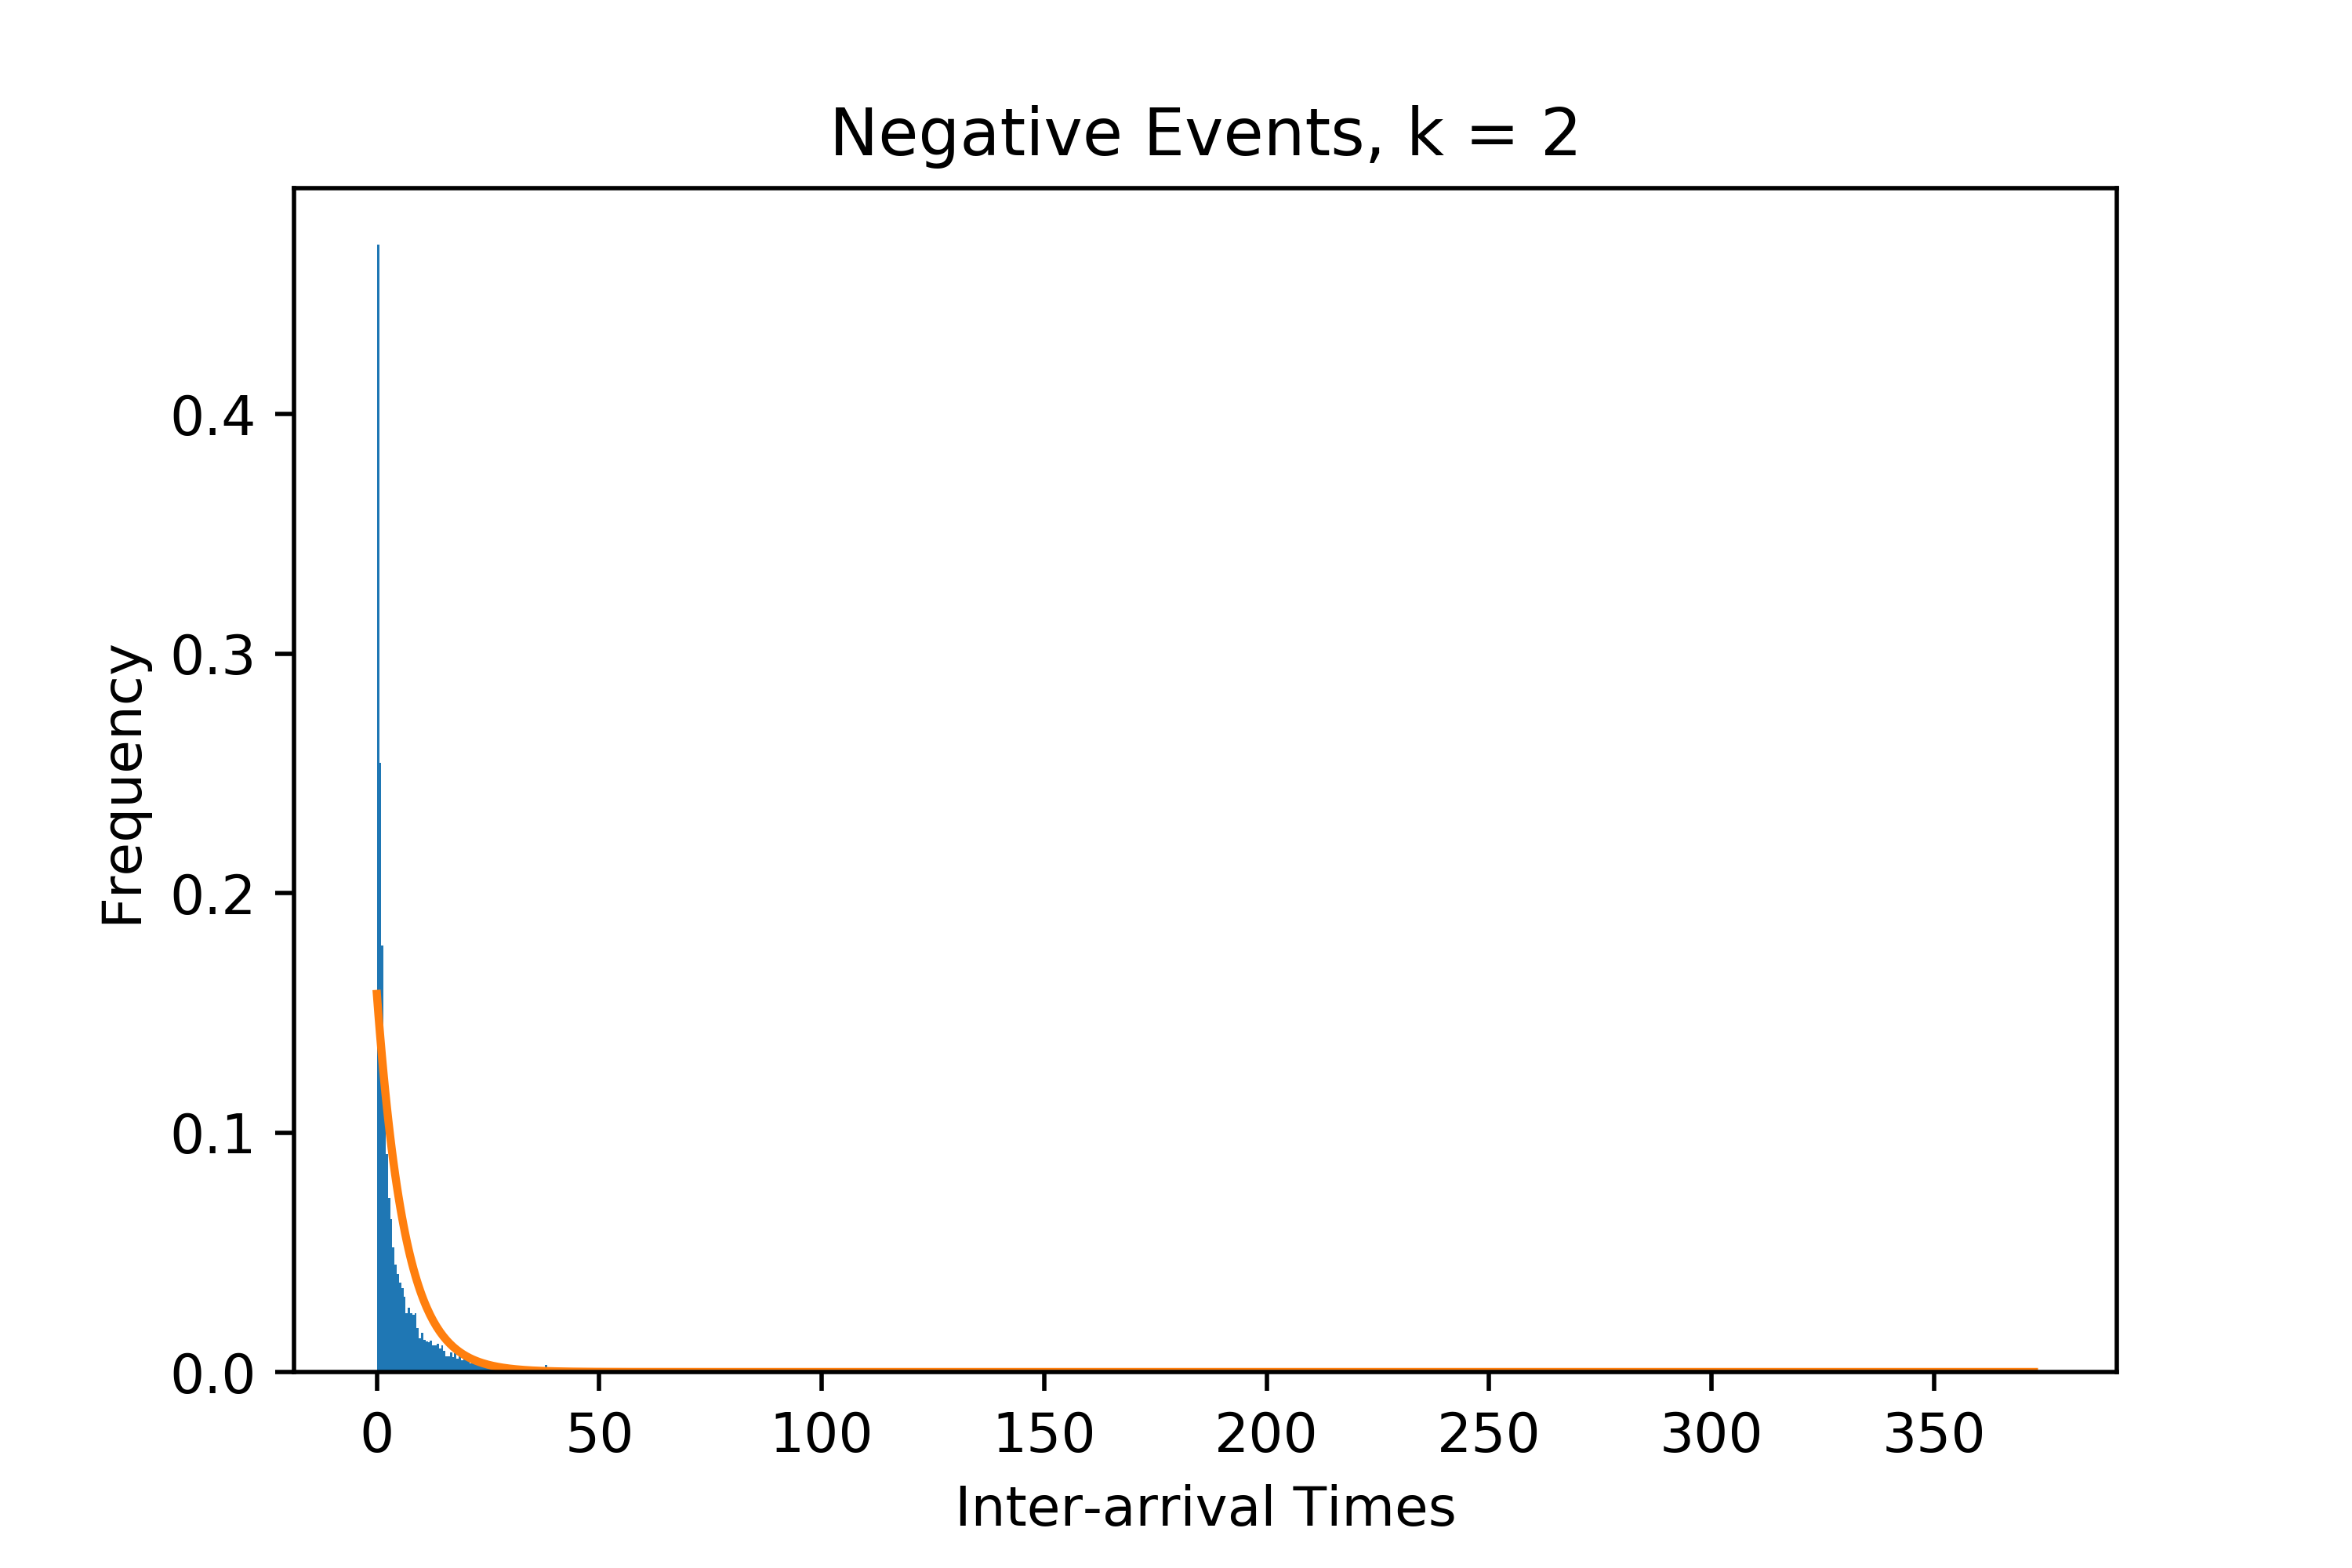
\includegraphics[width=60mm]{Figures/hist_neg_k2.png}}
{}
\\
\hline
\end{tabular}
\label{fig:interarrivals_neg}
\end{figure}

The products $\lambda^+_k \mu^+_k$ and $\lambda^-_k \mu^-_k$ can be thought of as the average rate of impact of positive and negative events. One concern with this model is that the impact of the positive events may overwhelm the impact of the negative events over time. That is, $\lambda^+_k \mu^+_k > \lambda^-_k \mu^-_k$ and $q^(k)^t$ is unbounded as simulation proceeds. This situation could arise since there could have a been an imbalance in the time frame of the data. We compare $\lambda^+_k \mu^+_k$ and $\lambda^-_k \mu^-_k$ in Table \ref{tab:parameters}. As can be seen, some rates are indeed larger for positive events compared to negative events. However, because the positive and negative rates are nearly the same at each position $q^(k)^t$ should not increase an unreasonable amount in a short simulation time frame.

\section{Arrival Correlations}\label{ch:correlations}
Although each of the marginal processes can be modelled as a Poisson process, I found that there were significant non-zero correlations between the arrivals at each position. Using a time period $t$ of 60 seconds, I found the correlation between $N^{\pm}_i(t)$ and $N^{\pm}_j(t)$ to generate $\sigma$ by sampling random intervals of length $t$ through the period of data collection. With $K=10$, $\sigma$ is a 40 by 40 matrix and is estimated with 160000 intervals using data from December 28-30. The code written to estimate these correlations is found in Listing \ref{correlation-code}.

The correlation matrix for positive events is shown in Table \ref{tab:pos_pos_corr_tab} where the entry $(i,j)$ is $corr(N^{+}_i(t), N^{+}_j(t))$. These correlations are visualized in figure \ref{fig:pos_pos_corr_pic}. In general, there are high positive correlations between events at a position $k$ and positions $k_{\pm 1}$, and to a lesser extent $k_{\pm 2}$ and $k_{\pm 3}$. The correlations between events near each suggests that activity near a price influences similar activity for nearby prices. The smaller positive correlations for positions far away from each other could be due different levels of activity in the market at different times. For example, there may be more trading activity and therefore more events across the board during work hours vs. nighttime hours.

\begin{table}
\caption{Correlation Matrix for $N^{+}_i(t), N^{+}_j(t)$, $t$ = 60 seconds} \label{tab:pos_pos_corr_tab}
\centering
\resizebox{\textwidth}{!}{\begin{tabular}{l|llllllllllllllllllll}
    & -10    & -9    & -8    & -7     & -6     & -5    & -4    & -3    & -2    & -1    & 1     & 2     & 3     & 4     & 5      & 6      & 7     & 8     & 9     & 10     \\ 
\hline
-10 & 1      & 0.349 & 0.247 & 0.231  & 0.203  & 0.166 & 0.13  & 0.138 & 0.05  & 0.072 & 0.09  & 0.07  & 0.045 & 0.047 & -0.002 & 0.019  & 0.073 & 0.079 & 0.081 & 0.094  \\
-9  & 0.349  & 1     & 0.439 & 0.301  & 0.232  & 0.167 & 0.123 & 0.138 & 0.113 & 0.133 & 0.149 & 0.136 & 0.096 & 0.05  & 0.016  & 0.022  & 0.062 & 0.091 & 0.157 & 0.115  \\
-8  & 0.247  & 0.439 & 1     & 0.6    & 0.435  & 0.265 & 0.198 & 0.221 & 0.098 & 0.141 & 0.162 & 0.159 & 0.086 & 0.036 & 0.011  & 0.029  & 0.064 & 0.09  & 0.2   & 0.095  \\
-7  & 0.231  & 0.301 & 0.6   & 1      & 0.629  & 0.318 & 0.159 & 0.189 & 0.044 & 0.143 & 0.143 & 0.16  & 0.121 & 0.019 & 0.021  & -0.019 & 0.029 & 0.107 & 0.125 & 0.061  \\
-6  & 0.203  & 0.232 & 0.435 & 0.629  & 1      & 0.639 & 0.298 & 0.23  & 0.045 & 0.134 & 0.195 & 0.205 & 0.172 & 0.093 & -0.003 & -0.012 & 0.039 & 0.108 & 0.131 & 0.07   \\
-5  & 0.166  & 0.167 & 0.265 & 0.318  & 0.639  & 1     & 0.529 & 0.344 & 0.142 & 0.2   & 0.255 & 0.222 & 0.212 & 0.156 & 0.089  & 0.06   & 0.071 & 0.089 & 0.129 & 0.07   \\
-4  & 0.13   & 0.123 & 0.198 & 0.159  & 0.298  & 0.529 & 1     & 0.539 & 0.235 & 0.229 & 0.241 & 0.232 & 0.224 & 0.204 & 0.15   & 0.143  & 0.143 & 0.11  & 0.149 & 0.1    \\
-3  & 0.138  & 0.138 & 0.221 & 0.189  & 0.23   & 0.344 & 0.539 & 1     & 0.395 & 0.248 & 0.239 & 0.256 & 0.237 & 0.206 & 0.128  & 0.134  & 0.184 & 0.143 & 0.184 & 0.11   \\
-2  & 0.05   & 0.113 & 0.098 & 0.044  & 0.045  & 0.142 & 0.235 & 0.395 & 1     & 0.333 & 0.221 & 0.205 & 0.164 & 0.133 & 0.127  & 0.147  & 0.18  & 0.125 & 0.171 & 0.108  \\
-1  & 0.072  & 0.133 & 0.141 & 0.143  & 0.134  & 0.2   & 0.229 & 0.248 & 0.333 & 1     & 0.276 & 0.213 & 0.193 & 0.233 & 0.219  & 0.184  & 0.195 & 0.149 & 0.172 & 0.111  \\
1   & 0.09   & 0.149 & 0.162 & 0.143  & 0.195  & 0.255 & 0.241 & 0.239 & 0.221 & 0.276 & 1     & 0.378 & 0.16  & 0.202 & 0.211  & 0.153  & 0.132 & 0.104 & 0.132 & 0.107  \\
2   & 0.07   & 0.136 & 0.159 & 0.16   & 0.205  & 0.222 & 0.232 & 0.256 & 0.205 & 0.213 & 0.378 & 1     & 0.473 & 0.21  & 0.171  & 0.14   & 0.132 & 0.16  & 0.146 & 0.092  \\
3   & 0.045  & 0.096 & 0.086 & 0.121  & 0.172  & 0.212 & 0.224 & 0.237 & 0.164 & 0.193 & 0.16  & 0.473 & 1     & 0.35  & 0.172  & 0.115  & 0.113 & 0.112 & 0.131 & 0.069  \\
4   & 0.047  & 0.05  & 0.036 & 0.019  & 0.093  & 0.156 & 0.204 & 0.206 & 0.133 & 0.233 & 0.202 & 0.21  & 0.35  & 1     & 0.271  & 0.138  & 0.101 & 0.064 & 0.097 & 0.057  \\
5   & -0.002 & 0.016 & 0.011 & 0.021  & -0.003 & 0.089 & 0.15  & 0.128 & 0.127 & 0.219 & 0.211 & 0.171 & 0.172 & 0.271 & 1      & 0.312  & 0.151 & 0.072 & 0.073 & 0.053  \\
6   & 0.019  & 0.022 & 0.029 & -0.019 & -0.012 & 0.06  & 0.143 & 0.134 & 0.147 & 0.184 & 0.153 & 0.14  & 0.115 & 0.138 & 0.312  & 1      & 0.293 & 0.118 & 0.101 & 0.087  \\
7   & 0.073  & 0.062 & 0.064 & 0.029  & 0.039  & 0.071 & 0.143 & 0.184 & 0.18  & 0.195 & 0.132 & 0.132 & 0.113 & 0.101 & 0.151  & 0.293  & 1     & 0.205 & 0.16  & 0.109  \\
8   & 0.079  & 0.091 & 0.09  & 0.107  & 0.108  & 0.089 & 0.11  & 0.143 & 0.125 & 0.149 & 0.104 & 0.16  & 0.112 & 0.064 & 0.072  & 0.118  & 0.205 & 1     & 0.195 & 0.13   \\
9   & 0.081  & 0.157 & 0.2   & 0.125  & 0.131  & 0.129 & 0.149 & 0.184 & 0.171 & 0.172 & 0.132 & 0.146 & 0.131 & 0.097 & 0.073  & 0.101  & 0.16  & 0.195 & 1     & 0.318  \\
10  & 0.094  & 0.115 & 0.095 & 0.061  & 0.07   & 0.07  & 0.1   & 0.11  & 0.108 & 0.111 & 0.107 & 0.092 & 0.069 & 0.057 & 0.053  & 0.087  & 0.109 & 0.13  & 0.318 & 1     
\end{tabular}}
\end{table}

\begin{figure}[t]
\begin{center}
\label{fig:pos_pos_corr_pic}
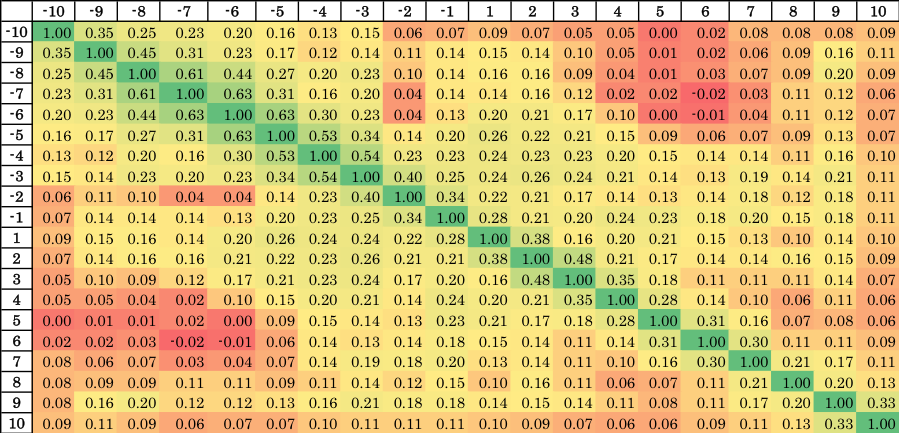
\includegraphics[width=0.8\textwidth]{LaTeX/Figures/pos_pos_correlations.png}
\caption{Correlation Matrix for $N^{+}_i(t), N^{+}_j(t)$, $t$ = 60 seconds}
\end{center}
\end{figure}

The correlation matrix for positive and negative events is shown in Table \ref{tab:pos_neg_corr_tab} where the entry $(i,j)$ is $corr(N^{+}_i(b), N^{-}_j(b))$. It is visualized in Figure \ref{fig:pos_neg_corr_pic}. Particularly notable is the very high (nearly 1) correlation between positive and negative at the same position. This could be due to traders reacting to updates by placing orders in the opposite direction, and could indicate that the order book is resilient to changes in the short term.

\begin{table}
\centering
\caption{Correlation Matrix for $N^{+}_i(t), N^{-}_j(t)$, $t$ = 60 seconds} \label{tab:pos_neg_corr_tab}
\resizebox{\textwidth}{!}{\begin{tabular}{l|llllllllllllllllllll}
    & -10   & -9    & -8    & -7     & -6     & -5    & -4    & -3    & -2    & -1    & 1     & 2     & 3     & 4     & 5     & 6      & 7     & 8     & 9     & 10     \\ 
\hline
-10 & 0.651 & 0.346 & 0.273 & 0.225  & 0.21   & 0.174 & 0.148 & 0.174 & 0.115 & 0.121 & 0.125 & 0.121 & 0.094 & 0.083 & 0.028 & 0.055  & 0.09  & 0.109 & 0.117 & 0.095  \\
-9  & 0.312 & 0.843 & 0.428 & 0.274  & 0.215  & 0.165 & 0.138 & 0.139 & 0.12  & 0.151 & 0.124 & 0.148 & 0.12  & 0.081 & 0.036 & 0.039  & 0.073 & 0.098 & 0.175 & 0.112  \\
-8  & 0.218 & 0.449 & 0.904 & 0.592  & 0.416  & 0.247 & 0.175 & 0.181 & 0.09  & 0.161 & 0.139 & 0.164 & 0.104 & 0.044 & 0.014 & 0.033  & 0.066 & 0.091 & 0.175 & 0.081  \\
-7  & 0.222 & 0.284 & 0.601 & 0.961  & 0.622  & 0.315 & 0.154 & 0.178 & 0.053 & 0.162 & 0.131 & 0.159 & 0.125 & 0.027 & 0.023 & -0.019 & 0.03  & 0.118 & 0.137 & 0.066  \\
-6  & 0.196 & 0.225 & 0.431 & 0.621  & 0.965  & 0.641 & 0.291 & 0.211 & 0.04  & 0.143 & 0.177 & 0.206 & 0.18  & 0.093 & 0.002 & -0.009 & 0.038 & 0.111 & 0.134 & 0.073  \\
-5  & 0.166 & 0.174 & 0.271 & 0.321  & 0.642  & 0.972 & 0.542 & 0.352 & 0.156 & 0.223 & 0.25  & 0.237 & 0.23  & 0.173 & 0.108 & 0.081  & 0.092 & 0.105 & 0.147 & 0.083  \\
-4  & 0.134 & 0.138 & 0.201 & 0.158  & 0.291  & 0.534 & 0.969 & 0.538 & 0.239 & 0.24  & 0.233 & 0.239 & 0.236 & 0.213 & 0.158 & 0.159  & 0.154 & 0.112 & 0.152 & 0.104  \\
-3  & 0.144 & 0.152 & 0.231 & 0.195  & 0.24   & 0.35  & 0.555 & 0.967 & 0.422 & 0.257 & 0.247 & 0.27  & 0.251 & 0.217 & 0.13  & 0.138  & 0.195 & 0.156 & 0.195 & 0.117  \\
-2  & 0.085 & 0.147 & 0.148 & 0.1    & 0.103  & 0.201 & 0.3   & 0.491 & 0.949 & 0.387 & 0.265 & 0.232 & 0.195 & 0.165 & 0.154 & 0.174  & 0.213 & 0.145 & 0.194 & 0.117  \\
-1  & 0.09  & 0.128 & 0.166 & 0.158  & 0.175  & 0.22  & 0.235 & 0.258 & 0.311 & 0.904 & 0.297 & 0.163 & 0.135 & 0.195 & 0.184 & 0.138  & 0.134 & 0.102 & 0.131 & 0.099  \\
1   & 0.048 & 0.159 & 0.135 & 0.102  & 0.136  & 0.196 & 0.196 & 0.182 & 0.213 & 0.304 & 0.925 & 0.396 & 0.181 & 0.207 & 0.224 & 0.161  & 0.148 & 0.117 & 0.14  & 0.112  \\
2   & 0.074 & 0.152 & 0.17  & 0.173  & 0.219  & 0.242 & 0.255 & 0.271 & 0.217 & 0.233 & 0.376 & 0.959 & 0.509 & 0.235 & 0.186 & 0.153  & 0.156 & 0.171 & 0.162 & 0.098  \\
3   & 0.045 & 0.095 & 0.089 & 0.116  & 0.168  & 0.215 & 0.23  & 0.246 & 0.182 & 0.214 & 0.171 & 0.488 & 0.98  & 0.368 & 0.19  & 0.129  & 0.128 & 0.116 & 0.14  & 0.077  \\
4   & 0.045 & 0.047 & 0.038 & 0.023  & 0.092  & 0.156 & 0.208 & 0.211 & 0.136 & 0.234 & 0.199 & 0.215 & 0.36  & 0.981 & 0.288 & 0.16   & 0.11  & 0.073 & 0.106 & 0.064  \\
5   & 0.002 & 0.013 & 0.008 & 0.023  & 0.002  & 0.09  & 0.152 & 0.128 & 0.118 & 0.208 & 0.217 & 0.162 & 0.168 & 0.273 & 0.984 & 0.313  & 0.149 & 0.072 & 0.074 & 0.049  \\
6   & 0.023 & 0.022 & 0.035 & -0.012 & -0.003 & 0.067 & 0.147 & 0.144 & 0.152 & 0.182 & 0.171 & 0.136 & 0.112 & 0.151 & 0.305 & 0.95   & 0.261 & 0.112 & 0.098 & 0.094  \\
7   & 0.085 & 0.096 & 0.086 & 0.05   & 0.069  & 0.095 & 0.156 & 0.204 & 0.185 & 0.198 & 0.166 & 0.141 & 0.107 & 0.099 & 0.141 & 0.258  & 0.944 & 0.195 & 0.17  & 0.121  \\
8   & 0.092 & 0.094 & 0.115 & 0.125  & 0.134  & 0.106 & 0.128 & 0.164 & 0.132 & 0.148 & 0.13  & 0.164 & 0.101 & 0.054 & 0.062 & 0.112  & 0.197 & 0.954 & 0.213 & 0.155  \\
9   & 0.096 & 0.174 & 0.231 & 0.158  & 0.172  & 0.158 & 0.176 & 0.207 & 0.157 & 0.151 & 0.152 & 0.155 & 0.134 & 0.093 & 0.068 & 0.091  & 0.125 & 0.212 & 0.809 & 0.26   \\
10  & 0.096 & 0.093 & 0.077 & 0.056  & 0.073  & 0.072 & 0.099 & 0.105 & 0.097 & 0.095 & 0.104 & 0.08  & 0.059 & 0.056 & 0.05  & 0.082  & 0.108 & 0.115 & 0.288 & 0.933 
\end{tabular}}
\end{table}

\begin{figure}[t]
\begin{center}
\label{fig:pos_neg_corr_pic}
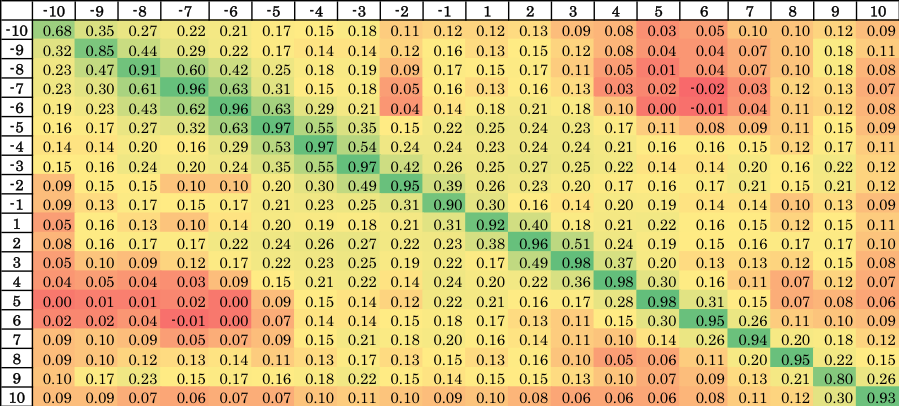
\includegraphics[width=0.8\textwidth]{LaTeX/Figures/pos_neg_correlations.png}
\caption{Correlation Matrix for $N^{+}_i(t), N^{-}_j(t)$, $t$ = 60 seconds}
\end{center}
\end{figure}


The correlation matrix for negative events is shown in Table \ref{tab:neg_neg_corr_tab} where the entry $(i,j)$ is $corr(N^{-}_i(b), N^{-}_j(b))$. It is visualized in Figure \ref{fig:neg_neg_corr_pic}. This matrix is similar in nature to the one for positive events, where positions near each other exhibit high correlations and there are lower positive correlations between positions that are further away from each other.

\begin{table}
\centering
\caption{Correlation Matrix for $N^{-}_i(t), N^{-}_j(t)$, $t$ = 60 seconds} \label{tab:neg_neg_corr_tab}
\resizebox{\textwidth}{!}{\begin{tabular}{l|llllllllllllllllllll}
    & -10    & -9    & -8    & -7     & -6     & -5    & -4    & -3    & -2    & -1    & 1     & 2     & 3     & 4     & 5      & 6      & 7     & 8     & 9     & 10     \\ 
\hline
-10 & 1      & 0.349 & 0.247 & 0.231  & 0.203  & 0.166 & 0.13  & 0.138 & 0.05  & 0.072 & 0.09  & 0.07  & 0.045 & 0.047 & -0.002 & 0.019  & 0.073 & 0.079 & 0.081 & 0.094  \\
-9  & 0.349  & 1     & 0.439 & 0.301  & 0.232  & 0.167 & 0.123 & 0.138 & 0.113 & 0.133 & 0.149 & 0.136 & 0.096 & 0.05  & 0.016  & 0.022  & 0.062 & 0.091 & 0.157 & 0.115  \\
-8  & 0.247  & 0.439 & 1     & 0.6    & 0.435  & 0.265 & 0.198 & 0.221 & 0.098 & 0.141 & 0.162 & 0.159 & 0.086 & 0.036 & 0.011  & 0.029  & 0.064 & 0.09  & 0.2   & 0.095  \\
-7  & 0.231  & 0.301 & 0.6   & 1      & 0.629  & 0.318 & 0.159 & 0.189 & 0.044 & 0.143 & 0.143 & 0.16  & 0.121 & 0.019 & 0.021  & -0.019 & 0.029 & 0.107 & 0.125 & 0.061  \\
-6  & 0.203  & 0.232 & 0.435 & 0.629  & 1      & 0.639 & 0.298 & 0.23  & 0.045 & 0.134 & 0.195 & 0.205 & 0.172 & 0.093 & -0.003 & -0.012 & 0.039 & 0.108 & 0.131 & 0.07   \\
-5  & 0.166  & 0.167 & 0.265 & 0.318  & 0.639  & 1     & 0.529 & 0.344 & 0.142 & 0.2   & 0.255 & 0.222 & 0.212 & 0.156 & 0.089  & 0.06   & 0.071 & 0.089 & 0.129 & 0.07   \\
-4  & 0.13   & 0.123 & 0.198 & 0.159  & 0.298  & 0.529 & 1     & 0.539 & 0.235 & 0.229 & 0.241 & 0.232 & 0.224 & 0.204 & 0.15   & 0.143  & 0.143 & 0.11  & 0.149 & 0.1    \\
-3  & 0.138  & 0.138 & 0.221 & 0.189  & 0.23   & 0.344 & 0.539 & 1     & 0.395 & 0.248 & 0.239 & 0.256 & 0.237 & 0.206 & 0.128  & 0.134  & 0.184 & 0.143 & 0.184 & 0.11   \\
-2  & 0.05   & 0.113 & 0.098 & 0.044  & 0.045  & 0.142 & 0.235 & 0.395 & 1     & 0.333 & 0.221 & 0.205 & 0.164 & 0.133 & 0.127  & 0.147  & 0.18  & 0.125 & 0.171 & 0.108  \\
-1  & 0.072  & 0.133 & 0.141 & 0.143  & 0.134  & 0.2   & 0.229 & 0.248 & 0.333 & 1     & 0.276 & 0.213 & 0.193 & 0.233 & 0.219  & 0.184  & 0.195 & 0.149 & 0.172 & 0.111  \\
1   & 0.09   & 0.149 & 0.162 & 0.143  & 0.195  & 0.255 & 0.241 & 0.239 & 0.221 & 0.276 & 1     & 0.378 & 0.16  & 0.202 & 0.211  & 0.153  & 0.132 & 0.104 & 0.132 & 0.107  \\
2   & 0.07   & 0.136 & 0.159 & 0.16   & 0.205  & 0.222 & 0.232 & 0.256 & 0.205 & 0.213 & 0.378 & 1     & 0.473 & 0.21  & 0.171  & 0.14   & 0.132 & 0.16  & 0.146 & 0.092  \\
3   & 0.045  & 0.096 & 0.086 & 0.121  & 0.172  & 0.212 & 0.224 & 0.237 & 0.164 & 0.193 & 0.16  & 0.473 & 1     & 0.35  & 0.172  & 0.115  & 0.113 & 0.112 & 0.131 & 0.069  \\
4   & 0.047  & 0.05  & 0.036 & 0.019  & 0.093  & 0.156 & 0.204 & 0.206 & 0.133 & 0.233 & 0.202 & 0.21  & 0.35  & 1     & 0.271  & 0.138  & 0.101 & 0.064 & 0.097 & 0.057  \\
5   & -0.002 & 0.016 & 0.011 & 0.021  & -0.003 & 0.089 & 0.15  & 0.128 & 0.127 & 0.219 & 0.211 & 0.171 & 0.172 & 0.271 & 1      & 0.312  & 0.151 & 0.072 & 0.073 & 0.053  \\
6   & 0.019  & 0.022 & 0.029 & -0.019 & -0.012 & 0.06  & 0.143 & 0.134 & 0.147 & 0.184 & 0.153 & 0.14  & 0.115 & 0.138 & 0.312  & 1      & 0.293 & 0.118 & 0.101 & 0.087  \\
7   & 0.073  & 0.062 & 0.064 & 0.029  & 0.039  & 0.071 & 0.143 & 0.184 & 0.18  & 0.195 & 0.132 & 0.132 & 0.113 & 0.101 & 0.151  & 0.293  & 1     & 0.205 & 0.16  & 0.109  \\
8   & 0.079  & 0.091 & 0.09  & 0.107  & 0.108  & 0.089 & 0.11  & 0.143 & 0.125 & 0.149 & 0.104 & 0.16  & 0.112 & 0.064 & 0.072  & 0.118  & 0.205 & 1     & 0.195 & 0.13   \\
9   & 0.081  & 0.157 & 0.2   & 0.125  & 0.131  & 0.129 & 0.149 & 0.184 & 0.171 & 0.172 & 0.132 & 0.146 & 0.131 & 0.097 & 0.073  & 0.101  & 0.16  & 0.195 & 1     & 0.318  \\
10  & 0.094  & 0.115 & 0.095 & 0.061  & 0.07   & 0.07  & 0.1   & 0.11  & 0.108 & 0.111 & 0.107 & 0.092 & 0.069 & 0.057 & 0.053  & 0.087  & 0.109 & 0.13  & 0.318 & 1     
\end{tabular}}
\end{table}

\begin{figure}[t]
\begin{center}
\label{fig:neg_neg_corr_pic}
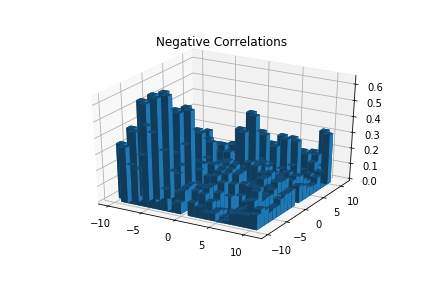
\includegraphics[width=0.8\textwidth]{LaTeX/Figures/neg_neg_correlations.png}
\caption{Correlation Matrix for $N^{-}_i(t), N^{-}_j(t)$, $t$ = 60 seconds}
\end{center}
\end{figure}

These non-zero correlations are clearly non-negligible, so I model the arrivals are a multivariate Poisson process where the arrivals are correlated and each marginal arrival distribution is Poisson. The correlations can be combined to form $\sigma$ as described. I will discuss the procedure for simulating the multivariate Poisson process in Chapter \ref{ch:simulation}.
